\chapter{循环神经网络}
\label{chap:recurrent-networks}

先看两类需要“记住过去”的任务。判断“这部电影并不精彩”的情感时，否定词“并不”与几步之后的“精彩”必须联系起来，孤立看任何一个词都会得出相反结论；预测设备下一时刻的温度，也往往要依据此前一段时间的升降趋势，而不只是当前读数。这类任务有两个共同特征：输入是\emph{陆续到达}的（一个词接一个词、一个时刻接一个时刻），而且序列长度\emph{可以变化}（评论有长有短）。第~\ref{chap:feedforward-networks}章的前馈网络要求输入是固定维度、一次性全部给出；第~\ref{chap:convolutional-networks}章的卷积虽然能处理网格，但固定层数和核尺寸只对应有限的历史窗口。于是本章要回答：\emph{当输入陆续到达、长度可变时，网络怎样把历史中有用的信息带到当前，又怎样从当前的错误反过来学会调整此前的处理}？

解决思路是引入一个随时间不断更新的内部变量——隐状态。它像一张“便签”：每读入一个新输入，就结合便签上原有的摘要和新内容，把便签改写一遍；做预测时只看这张便签即可，而不必保留所有历史输入。任务读出从便签形成当前预测，训练则根据当前误差去调整“改写便签”的规则。这一思路立刻引出三个贯穿全章、且彼此独立的问题：其一，\emph{信息}问题——便签容量有限，它是否真的容纳了任务所需的远期信息；其二，\emph{学习}问题——当错误在很晚才暴露时，梯度能否穿过许多次改写、传回负责记下远期信息的早期参数；其三，\emph{代价}问题——整段处理与逐步处理、保存全部历史与只维护定长状态，在计算和存储上各有什么取舍。

本章沿“历史经由隐状态传递”这一条共同机制展开。先用最普通的循环网络给出完整的递推、读出和训练过程（\ref{sec:rnn-basic}节）；随后看到普通网络难以保存远期信息，于是依次出现几种不同的改造思路：储备池干脆\emph{固定}状态动态、只学读出（\ref{sec:rnn-reservoir}节），LSTM、GRU用可学习的门\emph{选择性地}保存和覆盖（\ref{sec:rnn-gated}节），注意力不再把全部历史压进一个末状态、而是\emph{保存各位置表示}按需读取（\ref{sec:rnn-attention}节），状态空间模型则从线性递推与卷积、扫描的代数等价出发，改变历史的\emph{计算组织}（\ref{sec:rnn-state-space}节）。之后讨论双向、树结构等拓扑和深度扩展（\ref{sec:rnn-extensions}节），并在\ref{sec:rnn-theory}节从理论上区分表达、优化与泛化。需要提醒的是，这里的“时间步”不必是物理时间，也可以是词的位置、扫描次序或有向结构中的计算顺序。

\FloatBarrier
\section{循环神经网络概述}
\label{sec:rnn-overview}

在正式定义循环网络之前，先体会一下“不用记忆”时最直接的做法及其局限。要预测下一时刻，最简单的办法是把最近若干个观测拼成一个固定长度的向量，交给前馈网络。这个滑动窗口确实包含了顺序，却有两个硬伤：窗口以外的信息完全无法影响预测（无论多早发生的关键事件都被截断），而且改变窗口长度就要改变输入层的参数规模，网络结构随之变动。时间卷积用共享卷积核有所改善，但固定层数和核尺寸仍只对应一个有限的历史窗口，无法自然地“同一套计算一直运行下去”。我们真正想要的是：\emph{一个能随每个新输入持续更新、并把历史影响传递下去的内部变量}——这样无论序列多长，网络本身的参数和规模都不需要改变。

这个变量就是\term{隐状态}（hidden state）：它是网络根据已读输入逐步形成的内部摘要，不是训练样本直接给出的标签。设输入序列为$\bm{x}_1,\ldots,\bm{x}_T$，其中$\bm{x}_t\in\mathbb{R}^{d}$，长度$T$可以随样本改变。用$\bm{h}^{(t)}\in\mathbb{R}^{m}$表示读完第$t$个输入后的状态，\term{循环神经网络}（recurrent neural network, RNN）通过状态反馈，把前一步的内部表示用于下一步计算：
\begin{equation}
  \bm{h}^{(t)}=F_{\bm{\theta}}\!\left(\bm{h}^{(t-1)},\bm{x}_t\right),
  \qquad t=1,\ldots,T\text{。}
  \label{eq:rnn-general-recurrence}
\end{equation}
这里$F_{\bm{\theta}}$是具有参数$\bm{\theta}$的更新函数，$\bm{h}^{(0)}$是初始状态。下标$t$标识序列中的输入，上标$(t)$标识状态更新的步数；它们在本章按同一步对齐。状态的具体内容由更新函数和任务学习决定，可以是影响情感的否定，也可以是温度趋势；这条递推式只规定新状态从何处获得信息。

同一组$\bm{\theta}$在不同时间步复用，称为时间方向的\term{参数共享}（parameter sharing）。因此，延长序列会增加更新次数，却不必增加循环单元的参数量。\term{时间展开}（unrolling through time）则把这些更新依次画成计算图：第$t$步读取已经得到的第$t-1$步状态，展开图按已计算的旧状态逐步求值，形成有序的时间链。图~\ref{fig:rnn-unrolling}将状态反馈和展开图对应起来；展开后的深度随$T$增长，也是长序列训练困难的来源。

\begin{figure*}[htb]
  \centering
  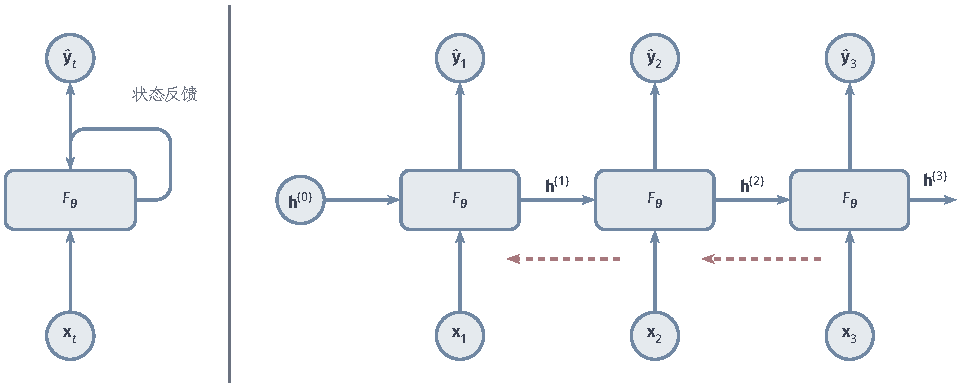
\includegraphics[width=162.810mm]{figures/05-neural-network-models/00-shared/tikz/rnn-unrolling/figure.pdf}
  \caption{状态递推的紧凑表示与时间展开。当前输入进入更新函数，隐状态沿时间传递，任务读出从状态形成预测。展开图中的$F_{\bm{\theta}}$是同一个更新函数的多次调用，参数共享而状态值不同。红色虚线示意较晚损失沿状态依赖回传梯度；图中只画三个更新步。}
  \label{fig:rnn-unrolling}
\end{figure*}
\FloatBarrier

循环网络的发展围绕两件事展开：怎样形成历史表示，以及怎样学到有用的状态更新。Elman在1990年的简单循环网络中，把前一步隐藏活动送回下一步，展示了这种上下文表示如何随序列任务形成。反馈在展开后成为一条时间链，同一参数因而可以作用于不同位置\scite{elman1990}

历史影响传到远处输出时，训练误差也要经过相应的多步依赖回传。Bengio、Simard和Frasconi在1994年分析了梯度学习与长期保留之间的困难：误差经多步状态变换回传时，影响可能迅速衰减或放大。这把研究重点从“网络是否含有反馈”推进到“反馈路径怎样传递信息与梯度”\scite{bengio1994rnn}

1997年的LSTM为持续记忆安排了单独的加性路径，后来加入的遗忘门使网络能够清除不再相关的内容。这条记忆通路与其他循环参数一起由任务目标训练。2001年的ESN和2002年的LSM则采用另一种分工：先构造通常固定的动态储备池，再学习任务读出。前一条路线让网络学习如何保存，后一条路线先提供历史特征；各自的原始工作和结构差别在第~\ref{sec:rnn-gated}节与第~\ref{sec:rnn-reservoir}节展开。

序列任务也推动了输出组织的变化。2014年，编码器—解码器使用一套循环网络读取源序列，另一套网络生成目标序列；Sutskever等用多层LSTM展示了这种端到端学习方式\scite{sutskever2014seq2seq} 同年的GRU用较少的门组织状态更新。随后，Bahdanau与Luong等的循环注意力模型让每个生成步骤重新读取编码器各位置的表示，减轻全部输入只能挤入同一末状态的限制。控制门改变保存方式，注意力改变读取方式，二者可以同时使用。

较新的状态空间路线还关心整段序列的计算组织。2020年的HiPPO把历史记忆写成在线投影问题；S4利用相应结构矩阵和快速核生成，在递推与卷积之间切换。2023年的Mamba把部分系数改为由输入产生，再通过选择性扫描计算；同年的RWKV以内容权重、时间衰减与定长累积量组织历史。第~\ref{sec:rnn-state-space}节将分别说明这些设计的原始形式。这些模型仍维护随输入更新的状态，并分别为状态构造、内容读取和计算执行安排结构。

本章按历史经由隐状态传递这一共同机制组织内容：链式循环、树递归、储备池以及基于隐状态递推的状态空间网络都在这里讨论。具体文献可能把状态空间网络单列为一类；各模型的具体更新函数和可训练参数在对应小节中另行给出。时间步也不必是物理时间，可以表示词的位置、扫描位置或有向结构中的计算次序。

\FloatBarrier
\section{基础循环神经网络}
\label{sec:rnn-basic}

本节先建立一个最普通的循环预测器，它由三组计算组成：\emph{状态更新}负责把新输入和旧状态概括成新状态，\emph{任务读出}规定在哪些位置、从状态产生什么预测，\emph{损失}衡量预测与目标的差距。理解这一节的关键是：同一套状态更新可以配不同的读出方式——可以只读最后一个状态给整段分类，也可以在每个位置都读出一个标签，还可以用两套网络在长度不等的序列之间转换。下面先给出共同的更新单元，再逐一介绍这些读出。

\subsection{网络结构}
\label{sec:rnn-structure}

普通RNN的更新规则非常直接：把当前输入和上一步状态各自线性映射后相加，再通过一个非线性函数。采用列向量约定，令
\begin{equation}
  \begin{aligned}
    \bm{z}^{(t)}&=\bm{U}\bm{x}_t+\bm{W}\bm{h}^{(t-1)}+\bm{b},\\
    \bm{h}^{(t)}&=\tanh\!\left(\bm{z}^{(t)}\right),\\
    \bm{a}^{(t)}&=\bm{V}\bm{h}^{(t)}+\bm{c},\qquad
    \widehat{\bm{y}}_t=g\!\left(\bm{a}^{(t)}\right)\text{。}
  \end{aligned}
  \label{eq:rnn-basic-cell}
\end{equation}
其中$\bm{U}\in\mathbb{R}^{m\times d}$决定新输入写入什么，$\bm{W}\in\mathbb{R}^{m\times m}$决定旧状态保留和混合多少，$\bm{b}\in\mathbb{R}^{m}$是隐藏偏置；$\bm{V}\in\mathbb{R}^{q\times m}$和$\bm{c}\in\mathbb{R}^{q}$从状态产生$q$维输出得分。这里用Tanh把状态限制在$(-1,1)$，既提供非线性又防止状态在反复递推中无界增大；它也可替换为其他激活，但梯度和状态范围会随之改变。$g$按任务选择恒等映射、Sigmoid或Softmax，输出与损失的配合沿用第~\ref{sec:ffn-output-objectives}节。

这里可以第一次看清循环网络为什么能用\emph{固定数量的参数}处理\emph{任意长度}的序列：$\bm U,\bm W,\bm b,\bm V,\bm c$这些参数与$T$完全无关，无论序列有多长，都只是反复套用同一个更新规则。代价则是计算必须按时间顺序进行——第$t$步依赖第$t-1$步的状态，天然难以并行。

这个单元及读出共有$md+m^2+m+qm+q$个参数，忽略逐坐标运算后，一步稠密计算的乘加量为$O(md+m^2+qm)$。长度为$T$的前向计算重复$T$次。固定宽度时，逐步预测只需维护当前状态；完整反向传播还需要沿途激活，或在求导时重算它们；保存这些激活时，训练存储随展开长度增加。

\subsubsection{序列到分类}
\label{sec:rnn-sequence-classification}

第一种读出对应“整段输入只有一个答案”的任务，如判断一整段评论是好评还是差评。网络把可变长度的评论逐步读入，但只在读完最后一个有效词后输出一次，因此称为\term{序列到分类}（sequence classification）。最直接的读出使用末状态：
\begin{equation}
  \bm{p}=\operatorname{softmax}\!\left(\bm{V}\bm{h}^{(T)}+\bm{c}\right),
  \qquad \ell=-\log p_y\text{，}
  \label{eq:rnn-classification}
\end{equation}
其中类别数为$K$、$q=K$、真实标签为$y\in\{1,\ldots,K\}$。末状态必须把与类别有关的信息带到结尾，所以较早出现的证据也要经过后续更新。

另一种读出对状态聚合，例如用$\overline{\bm{h}}=T^{-1}\sum_{t=1}^{T}\bm{h}^{(t)}$替代末状态。这里聚合的是已含历史的状态，仍然可以体现顺序；但平均会稀释只出现在少数位置的证据。末状态集中保留递推后的历史，平均分散各位置的影响，最大池化突出局部强响应，可学习聚合则按目标调整权重。标签依赖哪些位置，决定了这些读出各自需要保留的证据。


图~\ref{fig:rnn-sequence-classification}显示了末状态分类的监督位置：只有读完有效序列后，分类头才形成整段预测。
\begin{figure}[htb]
  \centering
  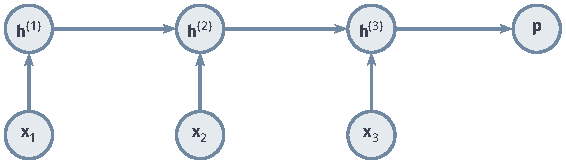
\includegraphics[width=95.793mm]{figures/05-neural-network-models/00-shared/tikz/rnn-sequence-classification/figure.pdf}
  \caption{序列到分类。三个输入依次更新同一循环单元，末状态产生类别概率$\bm p$。输入、隐状态与任务输出分列展示；图中只示意长度为3的序列。}
  \label{fig:rnn-sequence-classification}
\end{figure}
\FloatBarrier

\subsubsection{同步序列到序列}
\label{sec:rnn-aligned-sequences}

第二种读出对应“每个输入位置都要一个答案”，且输入与输出一一对齐，如给句子中每个词标注词性。\term{同步序列到序列}（aligned sequence-to-sequence）在每个有效位置都接上读出并计算损失：
\begin{equation}
  \ell=\frac{1}{T}\sum_{t=1}^{T}
  \ell_t\!\left(g(\bm{V}\bm{h}^{(t)}+\bm{c}),y_t\right)\text{。}
  \label{eq:rnn-aligned-loss}
\end{equation}
单向状态$\bm{h}^{(t)}$只读取$\bm{x}_1,\ldots,\bm{x}_t$。实时预测可以按这个可见范围运行。若任务允许读取整段输入，可以使用第~\ref{sec:rnn-topologies}节的双向结构补充后文信息。

时间预测也可以按位置组织，但要注明输出的时间含义。例如读入$\bm{x}_t$后预测$\bm{x}_{t+1}$，计算索引仍是$t$，目标却是下一步观测。这里的对齐指每个输入位置都接一个预测；目标的物理时刻由任务另外指定。


图~\ref{fig:rnn-aligned-sequences}在各位置设置读出；它与末状态分类共享同一种状态递推，但各位置都可以收到监督。
\begin{figure}[htb]
  \centering
  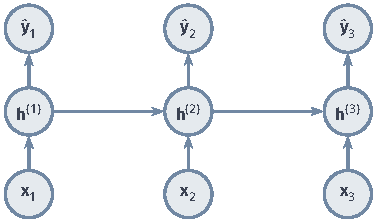
\includegraphics[width=63.793mm]{figures/05-neural-network-models/00-shared/tikz/rnn-aligned-sequences/figure.pdf}
  \caption{同步序列到序列。每个输入位置形成一个隐状态和相应预测。输入位置与预测位置对齐；若用于下一时刻预测，应另将目标移到后一时刻。图中单向状态只读取当前及此前输入。}
  \label{fig:rnn-aligned-sequences}
\end{figure}
\FloatBarrier

\subsubsection{异步序列到序列}
\label{sec:rnn-encoder-decoder}

第三种情形更一般：输出序列与输入序列\emph{长度不同、也没有天然的逐位置对应}，典型如机器翻译（一个英文词可能对应多个中文词、语序还要调整）。这时无法在每个输入位置上直接挂一个对齐的输出。\term{编码器—解码器}（encoder--decoder）把“读懂输入”和“产生输出”拆成两套循环网络：编码器先把整段输入读成一个上下文，解码器以此为条件，逐个生成目标符号。设目标长度为$S$，目标符号来自大小为$K$的词表，约定词表包含起止符号BOS和EOS。

解码器要把离散符号转换成向量输入，因此为每个符号保存一个$d_e$维的可学习向量，并将它们排成嵌入矩阵$\bm{E}\in\mathbb{R}^{d_e\times K}$。若$y$是符号的词表索引，\term{符号嵌入}（symbol embedding）就是查表取出的那一列，即$\bm{e}(y)=\bm{E}_{:,y}$；索引只用于选列，其数值大小不表示符号间的距离。用$\bm{s}^{(j)}$表示解码状态，基本形式为
\begin{equation}
  \begin{aligned}
    \bm{c}_{\mathrm{enc}}&=\bm{h}^{(T)},\qquad
    \bm{s}^{(0)}=\psi(\bm{c}_{\mathrm{enc}}),\\
    \bm{s}^{(j)}&=F_{\mathrm{dec}}\!\left(
      \bm{s}^{(j-1)},\bm{e}(y_{j-1}),\bm{c}_{\mathrm{enc}}\right),\\
    \bm{p}^{(j)}&=\operatorname{softmax}\!\left(
      \bm{V}_{\mathrm{dec}}\bm{s}^{(j)}+\bm{b}_{\mathrm{dec}}\right)\text{。}
  \end{aligned}
  \label{eq:rnn-encoder-decoder}
\end{equation}
$\psi$将编码状态映射到解码状态空间，编码器与解码器可以使用不同参数和宽度。起始符号$y_0=\mathrm{BOS}$为第一步提供输入，终止符号$\mathrm{EOS}$表示生成结束；它们也有各自的嵌入列。下文把$y_S=\mathrm{EOS}$计入目标序列。使用真实前缀训练时，$y_{j-1}$来自目标序列；生成时，它来自上一步概率分布中选出或采样的符号。两种情况都先查表得到$\bm{e}(y_{j-1})$再输入解码器；概率分布用于产生符号，符号索引用于取嵌入列。嵌入矩阵与其他网络参数一起通过训练更新。

目标序列的条件概率按生成次序分解：
\begin{equation}
  \begin{aligned}
    p_{\bm{\theta}}(y_{1:S}\mid\bm{x}_{1:T})
      &=\prod_{j=1}^{S}p_{\bm{\theta}}
        (y_j\mid y_{0:j-1},\bm{x}_{1:T}),\\
    \ell&=-\sum_{j=1}^{S}\log p^{(j)}_{y_j}\text{。}
  \end{aligned}
  \label{eq:rnn-sequence-likelihood}
\end{equation}
这里$y_{1:S}$、$\bm{x}_{1:T}$简记相应序列。条件中保留了此前目标，所以概率分解没有假设目标位置互相独立。对损失求和或按$S$平均，会分别让长序列包含更多损失项或先把各序列归一化，因而改变样本权重。

图~\ref{fig:rnn-encoder-decoder}将读取源序列与生成目标分开。两侧各画三个有效位置以便比较，并不要求实际源序列与目标序列等长。
\FloatBarrier
\begin{figure*}[t]
  \centering
  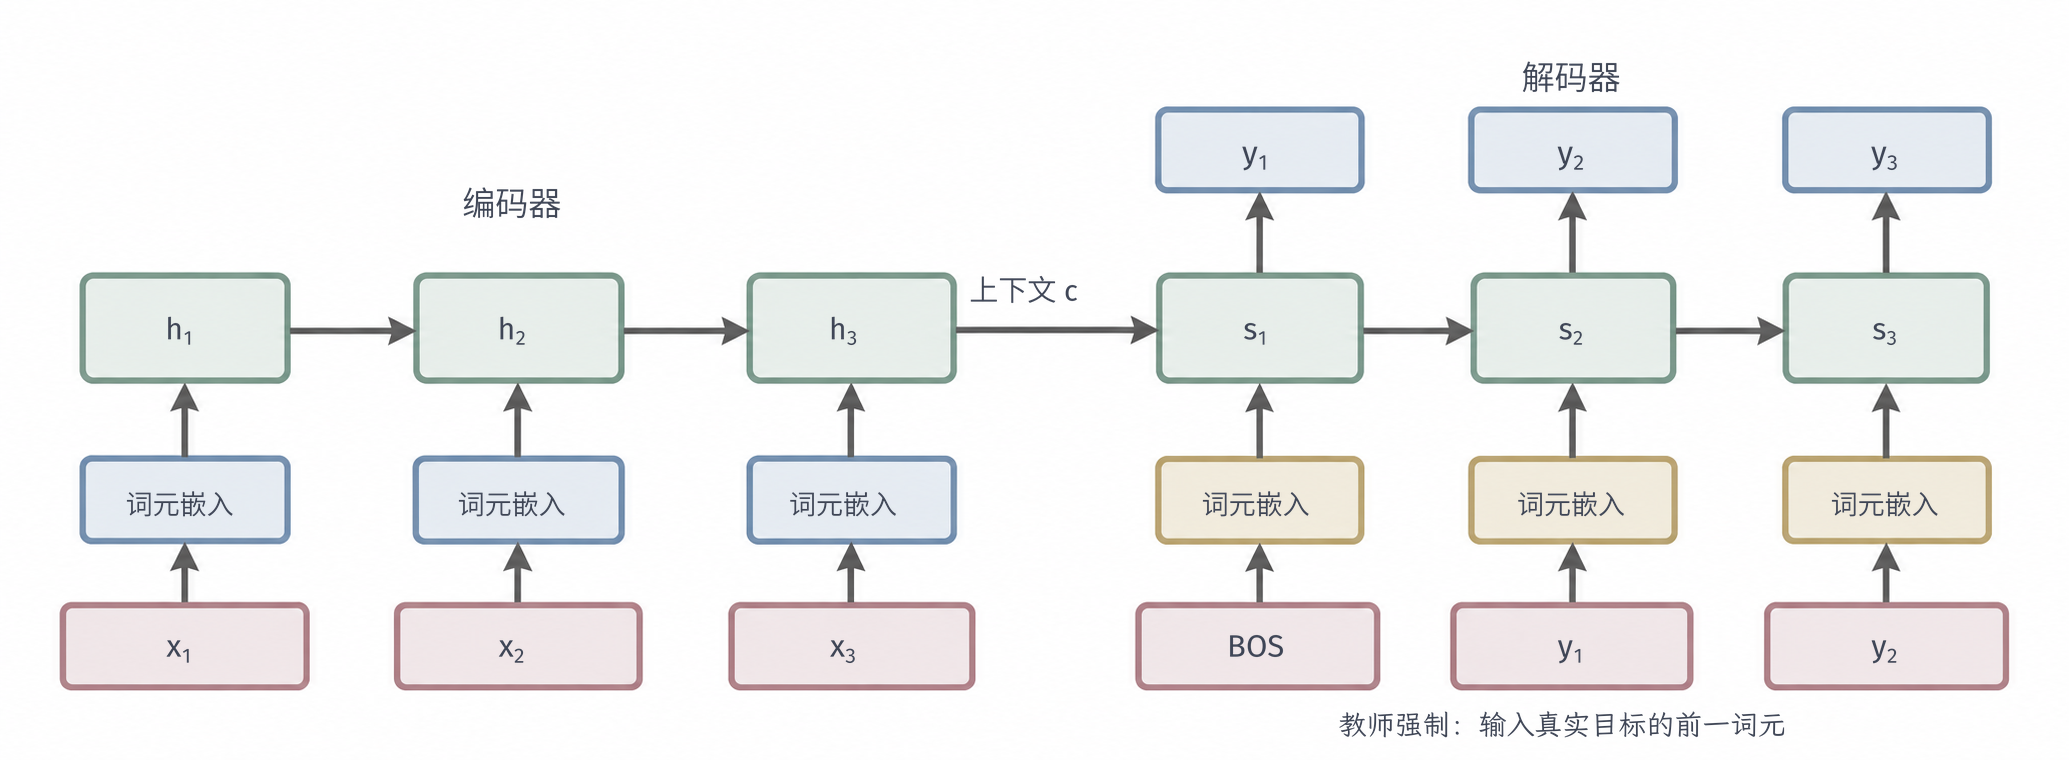
\includegraphics[width=169.000mm]{figures/05-neural-network-models/00-shared/generated/rnn-encoder-decoder/figure.png}
  \caption{异步序列到序列。编码器读取三个源输入，解码器在初态$\bm s^{(0)}$之后生成三个目标。BOS启动生成，右移后的目标经嵌入进入后续解码步。训练可使用真实目标，预测使用已生成目标；图中省略每步重复读取的固定上下文。}
  \label{fig:rnn-encoder-decoder}
\end{figure*}
\FloatBarrier

\subsection{参数学习}
\label{sec:rnn-learning}

循环网络的训练有两个区别于前馈网络的要点。第一，同一组参数在每个时间步都被使用，因此某个参数对总损失的影响，是它在\emph{所有时间步}上影响的总和，梯度必须沿时间累加。第二，循环矩阵$\bm W$被反复相乘，初始化时除了单步方差，还要关注多步连乘后信号是否被保持；正交初始化使初始的线性状态变换保持向量的欧氏范数，正是为了让信号在起点处既不快速放大也不快速缩小（激活导数仍会参与完整传播）。输入映射$\bm U$和输出映射$\bm V$可沿用第~\ref{sec:ffn-initialization}节的尺度原则。

状态的起点也要交代清楚。独立序列通常从一个固定的零状态，或同一个可学习的初始状态开始；若初态可学习，它的梯度同样由反向传播得到。在连续数据流上可以让状态跨批次延续，但前提是批次的每一行延续的是\emph{同一条}数据流；一旦换成无关样本，就必须重置状态。把上一条独立样本（比如上一篇评论）的隐状态带入下一条，等于让当前预测看到了不该看到的前文，会改变预测条件。

下面分别处理四个训练问题：怎样汇总共享参数在各时间步的梯度，怎样在长序列上控制存储和更新步长，怎样训练需要把输出反馈回来的序列模型，以及怎样维持跨很多步的梯度传播。前两项适用于一般循环训练；输出反馈取决于具体任务，长期依赖则需要进一步考察状态更新的动态。

\subsubsection{梯度计算与参数共享}
\label{sec:rnn-bptt}

循环网络带有“反馈环”，无法直接套用前馈网络逐层求导。一个关键技巧是\emph{时间展开}：把同一个更新函数在$T$个时间步上的调用依次画成一条首尾相连的长链——每一步都是一个“层”，相邻步之间传递状态。展开之后，它在数学上就等价于一个权重在各层之间\emph{共享}的很深的前馈网络，于是可以直接使用前两章的链式法则。这种沿时间展开图从后向前计算导数的方法，称为\term{随时间反向传播}（backpropagation through time, BPTT）。

以下以式\eqref{eq:rnn-basic-cell}为对象，令单序列目标为$L=\sum_{t=1}^{T}\ell_t$；没有监督的位置取$\ell_t=0$。记$\bm{g}^{(t)}=\partial\ell_t/\partial\bm{a}^{(t)}$，总损失对状态的梯度为$\bm{r}^{(t)}$，对预激活的梯度为$\bm{\delta}^{(t)}$，则
\begin{equation}
  \begin{aligned}
    \bm{r}^{(t)}&=\bm{V}^{\top}\bm{g}^{(t)}
       +\bm{W}^{\top}\bm{\delta}^{(t+1)},\\
    \bm{\delta}^{(t)}&=\bm{r}^{(t)}\odot
      \left(\bm{1}-\bm{h}^{(t)}\odot\bm{h}^{(t)}\right),
      \qquad \bm{\delta}^{(T+1)}=\bm{0}\text{。}
  \end{aligned}
  \label{eq:rnn-backward-recursion}
\end{equation}
$\odot$表示逐元素乘法。第一项来自当前读出，第二项来自后续状态；即使当前没有标签，后续损失仍可通过第二项监督这一步。若只在末状态分类，$t<T$的$\bm{g}^{(t)}$均为零，但相应$\bm{\delta}^{(t)}$未必为零。

每次调用都对共享参数产生一个局部贡献。求这一局部贡献时，将该步读入的上一状态视为独立输入；跨步依赖已由$\bm{\delta}^{(t)}$汇总，当前局部外积据此只计算本次调用对参数的影响。把所有调用的贡献累积起来，得到
\begin{equation}
  \begin{aligned}
    \nabla_{\bm{U}}L&=\sum_{t=1}^{T}\bm{\delta}^{(t)}\bm{x}_t^{\top},
    &\nabla_{\bm{W}}L&=\sum_{t=1}^{T}\bm{\delta}^{(t)}
      (\bm{h}^{(t-1)})^{\top},\\
    \nabla_{\bm{b}}L&=\sum_{t=1}^{T}\bm{\delta}^{(t)},
    &\nabla_{\bm{V}}L&=\sum_{t=1}^{T}\bm{g}^{(t)}(\bm{h}^{(t)})^{\top},\\
    \nabla_{\bm{c}}L&=\sum_{t=1}^{T}\bm{g}^{(t)},
    &\nabla_{\bm{h}^{(0)}}L&=\bm{W}^{\top}\bm{\delta}^{(1)}\text{。}
  \end{aligned}
  \label{eq:rnn-shared-gradients}
\end{equation}
这些梯度的形状与相应参数一致。自动微分沿所有调用位置汇总导数；这些位置共用一组参数，各步贡献更新的是同一对象。若目标按时间平均，相应梯度还需除以有效长度。

\begin{figure}[htbp]
  \centering
  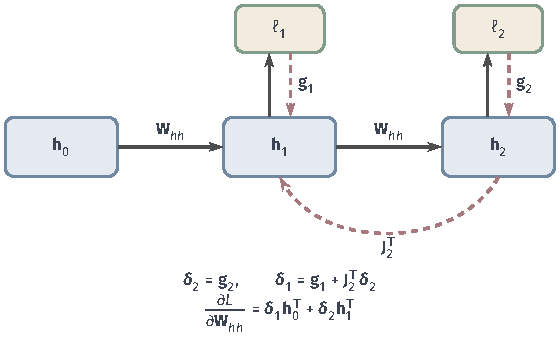
\includegraphics[width=94.756mm]{figures/05-neural-network-models/00-shared/tikz/rnn-bptt-two-steps/figure.pdf}
  \caption{两时间步BPTT的显式展开。蓝色实线是共享$\bm W_{hh}$的前向调用，红色虚线从$\ell_2$与$\ell_1$回传并在$\bm\delta_1$处汇合；同一循环矩阵的梯度等于两个调用位置的外积贡献之和。底部指出长序列中状态Jacobian连乘是梯度消失或爆炸的直接来源。}
  \label{fig:rnn-bptt-two-steps}
\end{figure}
\FloatBarrier

\begin{example}[两步递推中的梯度累积]
  \label{ex:rnn-shared-gradient}
  为单独观察共享参数，暂把Tanh换成恒等映射，使用标量更新$h^{(t)}=w h^{(t-1)}+x_t$；$w$是矩阵$\bm W$的一维情形。取固定初始状态$h^{(0)}=1$、$x_1=1$、$x_2=0$、$w=1/2$，只在末步计算损失$L=(h^{(2)})^2/2$。两次前向调用为
  \[
    \begin{aligned}
      h^{(1)}&=\tfrac12\times1+1=\tfrac32,\\
      h^{(2)}&=\tfrac12\times\tfrac32+0=\tfrac34\text{。}
    \end{aligned}
  \]
  反向从$r^{(2)}=h^{(2)}=3/4$开始，再沿第二步的状态依赖得到$r^{(1)}=w r^{(2)}=3/8$。本例激活导数为一，故$\delta^{(t)}=r^{(t)}$。第二次调用对$w$的局部导数是$h^{(1)}$，第一次是$h^{(0)}$，所以共享参数收到两项贡献：
  \[
    \begin{aligned}
      \frac{\mathrm dL}{\mathrm dw}
        &=r^{(1)}h^{(0)}+r^{(2)}h^{(1)}\\
        &=\tfrac38\times1+\tfrac34\times\tfrac32
          =\tfrac38+\tfrac98=\tfrac32\text{。}
    \end{aligned}
  \]
  第一项对应依赖路径$w\to h^{(1)}\to h^{(2)}\to L$，第二项对应$w\to h^{(2)}\to L$；梯度沿这些依赖逆向回传。两条路径的贡献最终相加，更新的仍是同一个$w$。直接展开$h^{(2)}=w(w+1)=w^2+w$，也有$\mathrm dL/\mathrm dw=(w^2+w)(2w+1)=3/2$，可与反向递推核对。

  若改取$h^{(0)}=0$，第一步对$w$的贡献为零，原因是$w$所乘的初态为零；共享参数仍在这一位置使用。若将本例的$h^{(0)}=1$改为可学习初态，它收到的梯度为$w r^{(1)}=3/16$，与$w$的梯度分开更新。
\end{example}

\subsubsection{长序列训练中的存储与更新控制}
\label{sec:rnn-truncation}

\paragraph{用截断限制反向传播的存储。}

长序列的完整展开会占用大量训练存储。\term{截断随时间反向传播}（truncated BPTT）把数据流分成有限长度的片段，在片段边界保留状态数值，却切断对更早计算的求导依赖。保留的状态数值仍把此前历史带入当前预测，求导则仅经过当前片段的更新。截断缩小了反向图，前向记忆仍由递推动态决定；遗漏跨边界路径后，所得梯度通常是完整梯度的有偏近似。

\paragraph{用裁剪限制过大的梯度。}

梯度过大时，可以在优化器更新之前使用\term{梯度裁剪}（gradient clipping），把梯度范数限制在阈值内。将全部参数梯度拼成$\bm{g}$，阈值为$\tau>0$，全局范数裁剪写为
\begin{equation}
  \widetilde{\bm{g}}=
  \begin{cases}
    \bm{g},&\lVert\bm{g}\rVert_2\leq\tau,\\
    \tau\bm{g}/\lVert\bm{g}\rVert_2,&\lVert\bm{g}\rVert_2>\tau\text{。}
  \end{cases}
  \label{eq:rnn-gradient-clipping}
\end{equation}
\Needspace{10\baselineskip}
对使用固定学习率的普通梯度下降，它保持非零梯度的方向并限制步长尺度，可减少异常大梯度造成的更新幅度。若学习率为$\eta>0$，参数增量为$\Delta\bm{\theta}=-\eta\widetilde{\bm{g}}$，故$\lVert\Delta\bm{\theta}\rVert_2=\eta\lVert\widetilde{\bm{g}}\rVert_2\leq\eta\tau$。对其他优化器，实际参数步幅还需结合其更新规则判断；式\eqref{eq:rnn-gradient-clipping}直接限制的是送入优化器的梯度范数。裁剪作用于已算出的参数梯度，早期影响若已衰减仍需从传播路径处理，前向状态动态也保持原定义。Pascanu等从状态Jacobian矩阵的乘积分析这两类梯度问题，并研究了裁剪的作用\scite{pascanu2013}

\paragraph{按样本边界与有效长度管理状态。}

可变长度批次常用填充补齐。\term{掩码}（mask）标记哪些位置是真实数据，使填充位置不参与损失或状态聚合。末状态读出使用每个样本的有效末位置；继续读取填充值会产生额外状态更新。平均聚合只汇聚有效位置，并以其数量作分母。

\subsubsection{自回归序列的训练与预测}
\label{sec:rnn-teacher-forcing}

这里出现一个训练与预测的不对称，是序列生成特有的关键问题。式\eqref{eq:rnn-sequence-likelihood}的条件概率默认每一步都以\emph{真实的}历史符号为前提；训练时确实可以把真实的$y_{j-1}$直接喂给第$j$步，这种做法称为\term{教师强制}（teacher forcing）：相当于老师在学生每写一个词时，都把正确的上文摆在他面前，让他专心学习“给定正确上文时下一个词该是什么”。但真正预测时并没有真实目标可用，第$j$步只能输入模型\emph{自己上一步生成}的符号；一旦早期生成错了，错误的前缀会把后续状态也带偏。于是训练时见到的前缀分布（总是正确）与预测时见到的前缀分布（可能含有错误）不一致，这种暴露偏差可能累积放大。

教师强制能直接、高效地优化真实序列的条件似然，因此仍是主流训练方式。若在训练中混入模型自己生成的符号，就改变了所学前缀的分布，需要相应地按新的生成过程建立学习目标，而不能简单套用。生成质量最终要在实际逐步预测的过程中评价：贪心解码每步选概率最大的符号；束搜索则同时保留若干个最有希望的候选前缀，但它覆盖的只是搜索空间的一部分，且受束宽限制。

\subsubsection{长期依赖中的梯度传播}
\label{sec:rnn-long-dependencies}

BPTT 揭示了普通RNN最致命的弱点，也解释了为什么本章后半部分需要那么多新结构。所谓\term{长期依赖}（long-term dependency），是指当前任务必须利用相隔很多步的信息——比如句首的主语决定句尾动词的形式。问题在于：较早的输入要影响很晚的输出，其影响必须\emph{连续穿过许多次状态更新}而存活下来；相隔多少步算“长”，要相对于模型实际能记住的有效尺度来判断。

把这件事写成数学语言。固定输入序列，记一步更新的状态\term{Jacobian矩阵}为$\bm{J}^{(t)}=\partial\bm{h}^{(t)}/\partial\bm{h}^{(t-1)}$，它描述“前一步状态的一个小扰动，经过这一步更新后变成多大”。链式法则给出从$s$步到$t$步的总影响
\begin{equation}
  \frac{\partial\bm{h}^{(t)}}{\partial\bm{h}^{(s)}}
    =\bm{J}^{(t)}\bm{J}^{(t-1)}\cdots\bm{J}^{(s+1)},
    \qquad t>s\text{。}
  \label{eq:rnn-jacobian-product}
\end{equation}
前向追踪“早期扰动能传多远”用这个乘积，反向传回损失梯度用它的转置，两者面对同样的连乘放大/衰减问题。普通Tanh单元中$\bm{J}^{(t)}=\bm{D}^{(t)}\bm{W}$，$\bm{D}^{(t)}$的对角元素为$1-(h_i^{(t)})^2$。注意Tanh在多数区域的导数都明显小于$1$（两端饱和时接近$0$），这使得连乘天然倾向于收缩。多步传播因此同时包含$\bm{W}$的线性作用、激活导数，以及不同步矩阵的相乘顺序。

若所有相关步都有$\lVert\bm{J}^{(t)}\rVert_2\leq r<1$，则乘积范数不超过$r^{t-s}$：每多走一步，早期信息能产生的影响就被乘以一个小于$1$的因子，呈指数衰减。\term{梯度消失}（vanishing gradients）使负责记录早期信息的参数几乎收不到有效更新——注意这与前馈网络中“层数多”导致的消失是同一类连乘机制，但在RNN中即使只有一个隐层，时间展开后也可能相当于成百上千层。反过来，若某些方向在多步乘积中持续被放大（$r>1$），则可能出现\term{梯度爆炸}（exploding gradients），一次更新把参数推得过远。单步范数只描述最强放大方向，多步中实际方向还会旋转变化；矩阵方向、激活饱和与当前输入共同决定沿具体轨迹的乘积。

\begin{example}[传播距离与状态保留]
  \label{ex:rnn-memory-decay}
  对线性标量递推$h^{(t)}=a h^{(t-1)}+x_t$，若$x_1=1$、后续输入为零且$h^{(0)}=0$，则$h^{(T)}=a^{T-1}$，跨步敏感度也为$a^{T-1}$。取$T=101$，$a=0.9$时为约$2.66\times10^{-5}$，$a=1.1$时为约$1.38\times10^4$。取$a=1$时，这个单一信号一直保留，多个输入则累加到同一状态中；任务读出还需要从累积结果区分所需历史。
\end{example}

式\eqref{eq:rnn-jacobian-product}包含两类因素：一条依赖路径经过多少次变换，以及每次变换怎样放大或衰减。控制路径长度与控制逐步增益，由此成为不同的结构设计。对一条含$\nu$次状态变换的路径，若各步范数不超过$r$，则
\begin{equation}
  \left\lVert\bm J_{\nu}\cdots\bm J_1\right\rVert_2
    \leq\prod_{k=1}^{\nu}\lVert\bm J_k\rVert_2\leq r^{\nu}\text{。}
  \label{eq:rnn-path-length-rate}
\end{equation}
$r$控制逐步变化的尺度，$\nu$控制这种变化重复多少次。这个范数上界控制路径上的最大放大程度；它也直接指明了改进长期依赖的\emph{三个不同着力点}，本章后续结构几乎都可归到其中之一：要么约束每一步的增益$r$（如正交初始化、固定储备池），要么缩短路径长度$\nu$（如跨时间跳跃、注意力的直达读取），要么让增益随内容自适应、在需要记忆时接近$1$（如LSTM、GRU的门）。下面据此分别考察逐步增益、路径长度和内容选择。

\paragraph{约束参数，控制逐步放大与衰减。}
\label{sec:rnn-parameter-constraints}

若传播方向的增益长期大于1，限制状态变换的范数可以减小指数放大；若增益长期小于1，只把范数压得更小反而会加重消失。保存长期影响需要相关方向的传播系数接近1，同时限制异常放大的方向。逐步增益的约束要同时满足这两类要求。

更强的条件同时约束最大和最小奇异值。若各步状态Jacobian矩阵的奇异值均在$[q,r]$内，$q>0$，对任意末端梯度$\bm v$有
\begin{equation}
  q^{\nu}\lVert\bm v\rVert_2
    \leq\left\lVert(\bm J_{\nu}\cdots\bm J_1)^{\top}\bm v\right\rVert_2
    \leq r^{\nu}\lVert\bm v\rVert_2\text{。}
  \label{eq:rnn-path-singular-bounds}
\end{equation}
使$q$与$r$都接近1，才同时抑制过快衰减与过快放大。普通Tanh单元的$\bm J^{(t)}=\bm D^{(t)}\bm W$还包含激活导数：即使约束$\bm W^{\top}\bm W=\bm I$，饱和的Tanh仍可使$\bm D^{(t)}$接近零。正交或酉矩阵约束保护的是线性部分，必须配合激活、输入尺度和完整Jacobian矩阵分析\scite{arjovsky2016unitary}

固定储备池是对可训练参数施加更强约束的一种做法。把循环动态参数$\bm\theta_{\mathrm{res}}$固定为$\bm\theta_0$，相当于将其可行集合限制为单点$\{\bm\theta_0\}$，任务训练只优化读出参数。储备池构造还常限制循环矩阵的尺度、连接和泄漏率，以安排状态的稳定性和记忆时间尺度。

冻结参数只限定训练的优化范围；前向动态的衰减或放大仍由这组固定参数决定。固定储备池的另一项作用，是训练时不再需要把末端错误沿长时间链传回循环参数，读出只需利用已经生成的状态特征。长距离任务梯度因此只需训练读出；任务相关历史是否到达读出，仍由固定动态提供的状态特征决定。

\paragraph{跨时间跳跃，减少路径上的变换次数。}
\label{sec:rnn-temporal-skips}

另一种做法增加从较早状态直接到较晚状态的边，例如
\begin{equation}
  \bm h^{(t)}=F_{\bm\theta}(\bm h^{(t-1)},\bm x_t)
       +\bm S\bm h^{(t-k)},\qquad t\geq k\text{，}
  \label{eq:rnn-temporal-skip}
\end{equation}
其中$k$是跳跃间隔，$\bm S\in\mathbb R^{m\times m}$是直达映射，边界状态另行初始化。从$t-k$到$t$的直接路径只经过$\bm S$。跨越距离$pk$时，沿连续跳跃边的一条路径经过$p$次变换；在$\lVert\bm S\rVert_2\leq r$下，该路径的范数上界为$r^p$，普通逐步路径则可能含$pk$次变换。

在标量教学例子中，同样以$0.9$为路径系数，跨100步的逐步路径为$0.9^{100}\approx2.66\times10^{-5}$，每10步跳一次的路径为$0.9^{10}\approx0.349$。这是新增路径的比较；完整梯度包含所有路径贡献的和，单一路径的$r^{\nu/k}$只是其中的传播尺度。跳跃也需要保存相应旧状态，并可能跳过任务所需的细粒度处理。

跨层残差改变层方向路径，跨时间跳跃改变时间方向依赖。直达路径之外，其他分支和多路径相加也参与梯度；状态中的目标信息还需要由读出提取。

\paragraph{使用控制门，按内容调节保留率。}
\label{sec:rnn-gated-memory-path}

固定约束对所有输入使用同一规则，任务却可能只需保存某些内容。控制门把保留系数变成输入相关量。LSTM中，$f_i^{(u)}\in(0,1)$表示第$u$步第$i$个记忆坐标的遗忘门值。以LSTM的直接记忆路径为例，暂固定门的数值后，从$s$到$t$的逐坐标系数为$\prod_{u=s+1}^{t}f_i^{(u)}$。由于每一步都把旧记忆的这个坐标乘以当步门值，跨步保留的系数就逐步相乘。需要保存时令相应遗忘门接近1，需要覆盖时降低它；输入门再调节新内容写入。门控主要改变逐步保留率与信息通路，通常没有减少时间步数。

门本身也依赖状态，完整Jacobian矩阵还包含门与候选变化的路径。能建立接近恒等的记忆通路，为训练提供了选择，任务损失仍需学到何时使用它。第~\ref{sec:rnn-lstm}节和第~\ref{sec:rnn-gru}节将把这些路径写成具体单元。

这几类方式可以组合：固定储备池也能加入跳跃连接，门控网络也能约束部分矩阵。传播路径、逐步增益、可训练参数范围和读出所需信息，分别描述这些组合实际改变了什么。

\FloatBarrier
\section{基于储备池的循环神经网络}
\label{sec:rnn-reservoir}

普通RNN用BPTT学习循环参数，但前面的Jacobian分析表明，让循环动态既稳定又可训练非常困难。\term{储备池计算}（reservoir computing）采用一种近乎“放弃治疗”却出人意料有效的分工：\emph{既然学习复杂的循环动态这么难，那就干脆不学时序部分，只学最后的读出}。具体做法是构造一个通常固定、且足够丰富的非线性动态系统，让它把输入历史自动映射成一组高维、随时间变化的状态特征；这些特征已经隐含了历史的各种回声和组合，再接一个简单的（往往是线性的）\emph{读出}层，只训练读出层去完成任务。这里的\term{读出}（readout）就是任务输出映射：接收状态特征，计算回归值或类别概率。状态随输入不断改变，但产生状态的循环参数不按当前任务的梯度更新。图~\ref{fig:rnn-reservoir}展示了这一分工。

这种分工为什么可行？直觉上，一个构造得当的高维随机动态系统会像“回声室”一样，把每一段不同的历史输入投射成彼此可区分的当前状态——历史越近影响越大，但足够慢的衰减使远期信息也留下痕迹。只要这些状态特征能区分任务所需的不同历史，一个线性读出往往就足以从中挑出答案；困难的时序特征工程由此被转化为一个简单的静态拟合问题。它尤其适合难以对长循环链做梯度训练、但能接受线性读出能力上限的场景。

\begin{figure*}[htb]
  \centering
  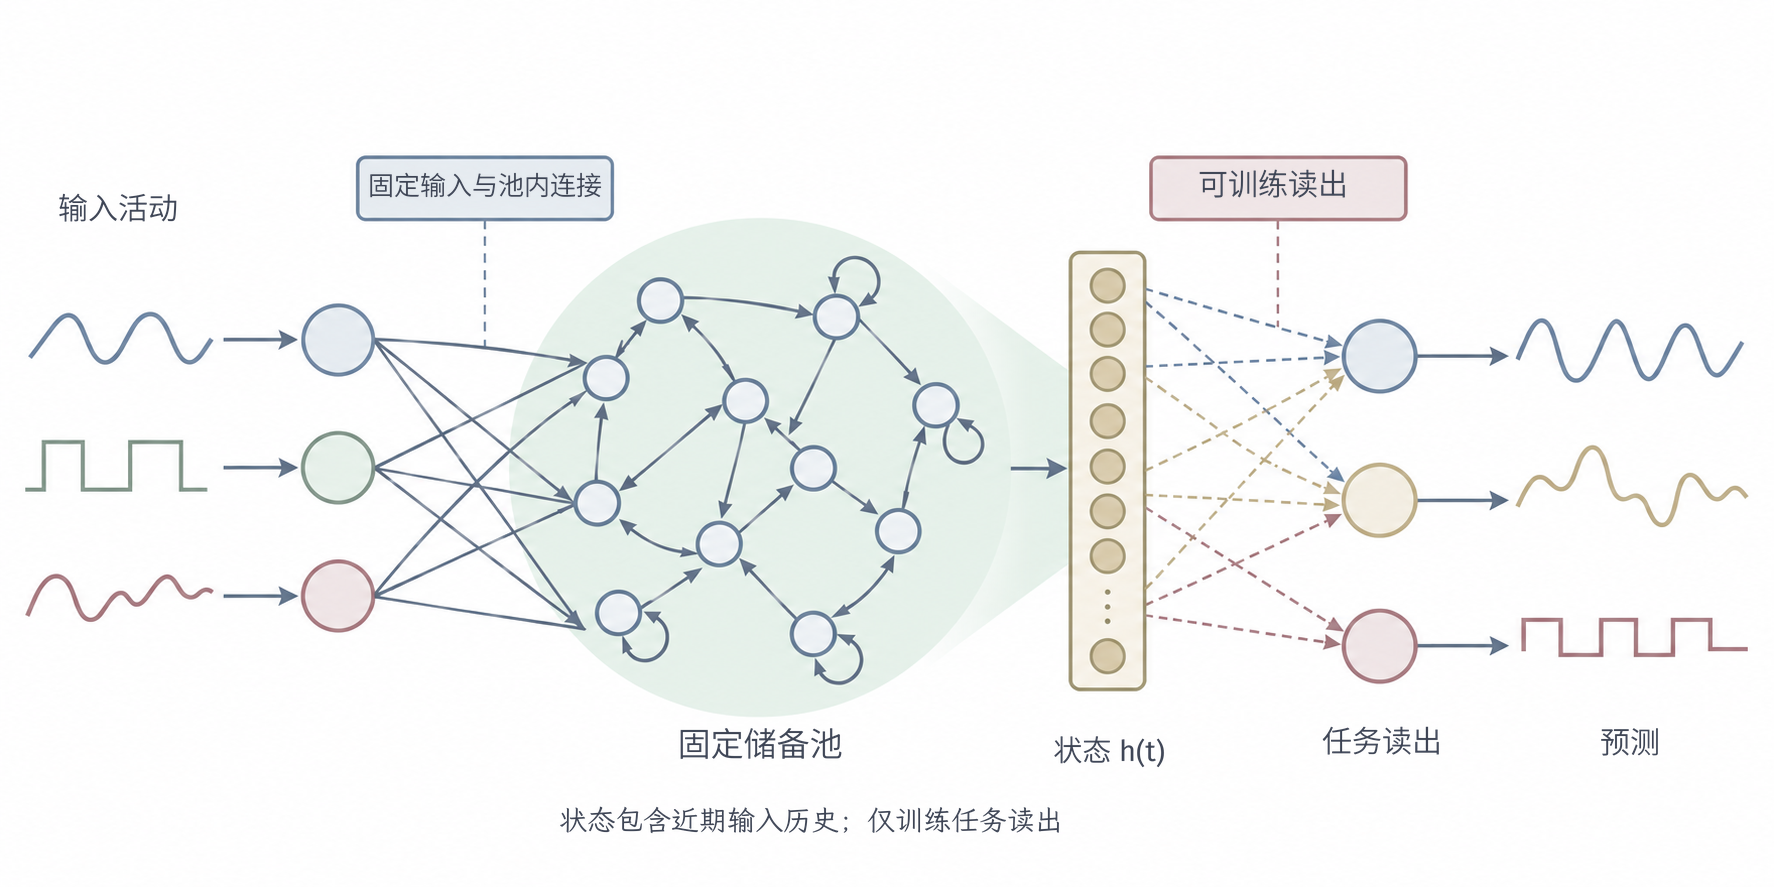
\includegraphics[width=150.199mm]{figures/05-neural-network-models/00-shared/generated/rnn-reservoir/figure.png}
  \caption{储备池计算的参数分工。输入进入固定的循环动态，多个内部单元共同形成随历史变化的状态，可训练读出将状态映射到目标。灰色连线表示固定连接，箭头表示参与拟合的读出；内部连接只示意结构，不表示某个随机生成样本。ESN使用连续值激活，LSM可由脉冲活动及其滤波响应形成读出特征。}
  \label{fig:rnn-reservoir}
\end{figure*}
\FloatBarrier

\subsection{ESN}
\label{sec:rnn-esn}

\term{回声状态网络}（echo state network, ESN）是一种以连续值循环状态提供历史特征的储备池模型，Jaeger的技术报告建立了其基本框架\scite{jaeger2001} 下面采用无输出反馈的泄漏积分版本，避免把真实目标或读出结果再送入储备池。令泄漏率$\alpha\in(0,1]$，更新为
\begin{equation}
  \begin{aligned}
    \widetilde{\bm{h}}^{(t)}&=\tanh\!\left(
      \bm{W}_{\mathrm{res}}\bm{h}^{(t-1)}
      +\bm{U}_{\mathrm{res}}\bm{x}_t+\bm{b}_{\mathrm{res}}\right),\\
    \bm{h}^{(t)}&=(1-\alpha)\bm{h}^{(t-1)}
       +\alpha\widetilde{\bm{h}}^{(t)}\text{。}
  \end{aligned}
  \label{eq:rnn-esn-update}
\end{equation}
$\bm{W}_{\mathrm{res}}\in\mathbb{R}^{m\times m}$、$\bm{U}_{\mathrm{res}}\in\mathbb{R}^{m\times d}$和偏置通常构造后固定。较小$\alpha$使每次状态变化较慢，但实际记忆还取决于循环矩阵、输入尺度和非线性响应。稀疏连接、输入缩放、泄漏率和状态维度均是可由验证选择的配置。

训练时先运行储备池，收集特征$\bm{z}_t=[1;\bm{x}_t;\bm{h}^{(t)}]\in\mathbb{R}^{1+d+m}$，分号表示向量拼接。初始若干步可能主要反映人为初态，常丢弃这段\term{洗出期}（washout），即先让系统接受输入、再开始拟合读出。洗出期剔除的是受初态影响的读出特征，任务标签所依赖的输入仍要进入状态更新；独立序列采用一致的洗出和重置规则。

对连续值目标，将$N$个有效状态按行堆成$\bm{Z}\in\mathbb{R}^{N\times(1+d+m)}$，相应目标堆成$\bm{Y}\in\mathbb{R}^{N\times q}$。线性读出参数为$\bm{R}\in\mathbb{R}^{(1+d+m)\times q}$，采用平方损失和岭惩罚时
\begin{equation}
  \begin{aligned}
    \bm{R}^{\star}&=\argmin_{\bm{R}}
      \lVert\bm{Z}\bm{R}-\bm{Y}\rVert_{\mathrm{F}}^2
      +\lambda\lVert\bm{R}\rVert_{\mathrm{F}}^2,\\
    \bm{R}^{\star}&=(\bm{Z}^{\top}\bm{Z}+\lambda\bm{I})^{-1}
      \bm{Z}^{\top}\bm{Y},\qquad \lambda>0\text{。}
  \end{aligned}
  \label{eq:rnn-esn-ridge}
\end{equation}
这里$\lVert\cdot\rVert_{\mathrm{F}}$是Frobenius范数。公式惩罚了包括截距在内的全部系数；若不惩罚截距，应改用相应对角惩罚矩阵并另查可逆性。实现时可解对应线性方程，公式中的逆矩阵表示其解。Softmax与交叉熵读出则产生另一种目标，按分类目标训练参数。

拟合出的$\bm{R}^{\star}$按列保存各输出坐标的权重。对列特征向量$\bm{z}_t$，连续值预测为$\widehat{\bm{y}}_t=(\bm{R}^{\star})^{\top}\bm{z}_t\in\mathbb{R}^{q}$；这与设计矩阵按行保存特征、$\bm{Z}\bm{R}^{\star}$逐行给出预测的约定一致。训练后将固定储备池的配置与拟合出的读出参数一同保存。处理新的独立序列时，按训练时约定的初始化、洗出和特征构造规则运行同一储备池，在有效读出位置用$\bm{R}^{\star}$形成预测；处理同一连续流时，则按约定延续状态。

任务读出希望状态主要由输入历史决定，初态差异随持续输入逐渐减弱。\term{回声状态性质}（echo state property, ESP）要求在约定的输入与状态范围内，相同持续输入驱动下，初始状态的影响最终消失。对式\eqref{eq:rnn-esn-update}，Tanh是1-Lipschitz，因而两个状态的距离满足
\begin{equation}
  \lVert\bm{h}^{(t)}-\bm{h}_{\mathrm{alt}}^{(t)}\rVert_2
    \leq\left(1-\alpha+\alpha\lVert\bm{W}_{\mathrm{res}}\rVert_2\right)
      \lVert\bm{h}^{(t-1)}-\bm{h}_{\mathrm{alt}}^{(t-1)}\rVert_2\text{。}
  \label{eq:rnn-esn-contraction}
\end{equation}
这里$\bm{h}^{(t)}$与$\bm{h}_{\mathrm{alt}}^{(t)}$表示初态不同、输入相同的两条轨迹。$\lVert\bm{W}_{\mathrm{res}}\rVert_2<1$给出统一收缩的充分条件，但不是必要条件。按谱半径缩放限制线性模式，非线性储备池还包含激活和输入驱动；相关反例与更精确条件见Yildiz等的分析\scite{yildiz2012}

初态影响消失也意味着一部分过去影响会衰减，适当的衰减使模型能适应新输入，过快衰减却可能丢掉任务证据。\term{记忆容量}（memory capacity）的一种线性测量方法，是对独立同分布的零均值标量输入，在方差有限且非零的条件下，分别学习各延迟的线性重构，再累加平方相关系数。若某个延迟的总体最小二乘重构量方差为零，通常的相关系数分母也为零；本文约定将该延迟的容量贡献按0计，表示这份线性重构没有恢复输入的变化。在状态为$m$维、读出仅使用状态且采用相应总体最小二乘定义的条件下，总线性记忆容量不超过$m$；这项容量指标衡量线性延迟重构，任务分类的准确率由相应目标另外评价\scite{jaeger2001memory} 读出优化利用已有特征，远期证据是否仍可区分则要从动态状态检验。

\subsection{LSM}
\label{sec:rnn-lsm}

输入也可能由带时间戳的事件构成，如传感器事件或神经脉冲。\term{液态状态机}（liquid state machine, LSM）用动态储备池的瞬时响应表示输入历史，代表性实现是固定的脉冲神经元回路，再学习状态读出。其名称强调利用持续变化的内部活动，不要求系统每次都收敛到一个稳定状态。

图~\ref{fig:rnn-lsm}把输入到任务输出的过程分开。输入是事件时，可以直接接入脉冲回路；连续观测则需按约定编码为输入脉冲。编码规则决定观测幅度、变化或时间如何转成回路接受的事件输入。
\begin{figure*}[htb]
  \centering
  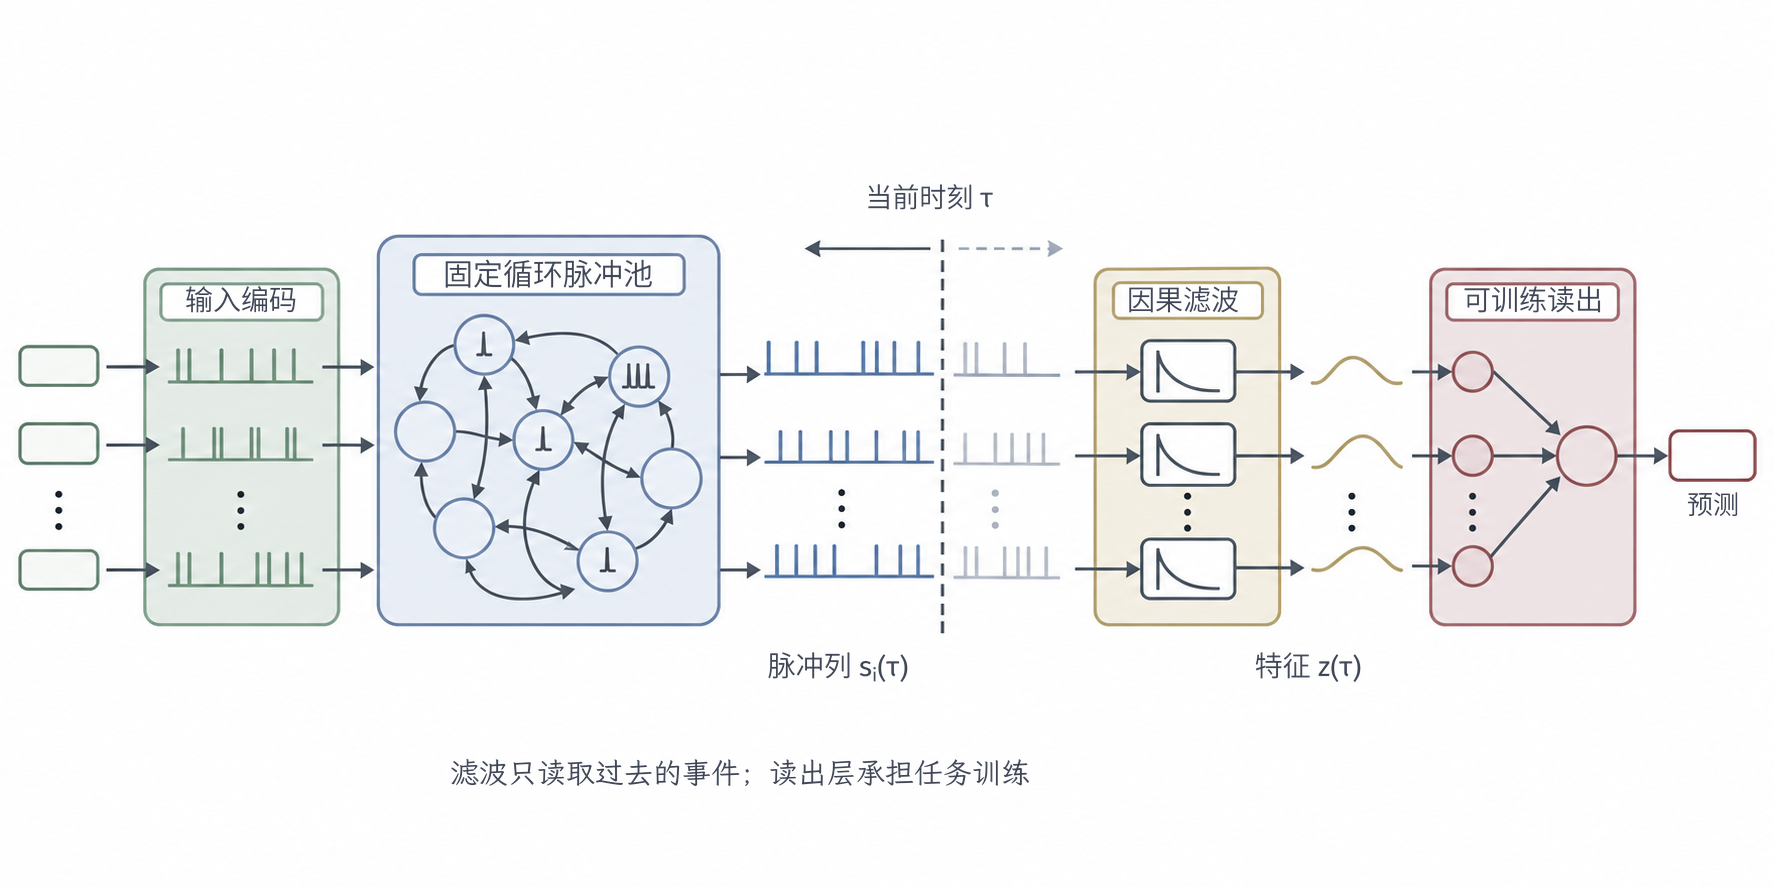
\includegraphics[width=150.199mm]{figures/05-neural-network-models/00-shared/generated/rnn-lsm/figure.png}
  \caption{LSM的输入、动态与读出。输入编码驱动固定的循环脉冲储备池，回路活动形成脉冲列$s_i(\tau)$；因果滤波将这些活动变成当前可读特征$\bm z(\tau)$，任务读出再映射为预测。反馈表示回路动态，滤波后的特征进入可训练任务读出。此处只训练任务读出，脉冲编码、回路参数与滤波核按约定固定。}
  \label{fig:rnn-lsm}
\end{figure*}
\FloatBarrier

回路中的状态比“这个时刻是否发出脉冲”更丰富。例如一个简化的漏积分发放单元可以写为
\begin{equation}
  \tau_{\mathrm m}\frac{\mathrm d v_i(\tau)}{\mathrm d\tau}
    =-(v_i(\tau)-v_{\mathrm{rest}})
      +I_i(\tau)+\sum_j w_{i,j}(\kappa_{\mathrm{syn}}*s_j)(\tau)\text{，}
  \label{eq:rnn-lsm-membrane}
\end{equation}
其中$v_i$是膜电位，$v_{\mathrm{rest}}$是静息电位，$\tau_{\mathrm m}>0$是泄漏时间常数，$I_i$表示换算到同一电位尺度的外部驱动，$w_{i,j}$是固定连接权重，$\kappa_{\mathrm{syn}}*s_j$是此前脉冲经过突触滤波后的作用。膜电位达到阈值时发出脉冲并重置；这里省略不应期等细节。持续的膜电位、突触响应和反馈活动共同承载输入历史，当前输入停止后，内部影响仍可能延续\scite{maass2002}

若第$i$个单元在时刻$\tau_{i,k}$发出脉冲，其脉冲列为$s_i(\tau)=\sum_k\delta(\tau-\tau_{i,k})$，$\delta$是Dirac脉冲。它不是某一时刻的普通有限函数值，而是用积分记录一次单位事件：与连续权重函数相乘后积分，就取出该函数在发放时刻的值。因而可以用因果滤波核$\kappa_i$形成特征：
\begin{equation}
  z_i(\tau)=\int_{-\infty}^{\tau}\kappa_i(\tau-u)s_i(u)\,\mathrm du,
  \qquad \kappa_i(v)=e^{-v/\tau_i}\mathbf 1_{\{v\geq0\}}\text{。}
  \label{eq:rnn-lsm-filter}
\end{equation}
$\tau_i>0$是特征衰减时间常数，$\mathbf 1$是指示函数。采用事件发生后立即计入当前状态的约定，积分可以逐个发放时刻展开为
\begin{equation}
  z_i(\tau)=\sum_{k:\,\tau_{i,k}\leq\tau}
    \exp\!\left(-\frac{\tau-\tau_{i,k}}{\tau_i}\right)\text{。}
  \label{eq:rnn-lsm-event-sum}
\end{equation}
每次脉冲向$z_i$加入$1$，此后按已经过去的时间衰减；未来事件不参与求和。脉冲编码的进一步说明见第~\ref{sec:snn-coding}节。这一步是状态读取：把回路活动整理成有限维、可供后续计算的$\bm z(\tau)$。这些滤波特征保留了所选脉冲响应，膜电位和其他突触变量仍可能未被记录；读出获得的信息范围由所选特征决定。

读出是从这些状态特征到任务预测的映射，作用相当于前馈网络的输出头。读取特征与产生任务答案是两步计算；一个常用读出为
\begin{equation}
  \bm a(\tau)=\bm V\bm z(\tau)+\bm b,
  \qquad\widehat{\bm y}(\tau)=g(\bm a(\tau))\text{，}
  \label{eq:rnn-lsm-readout}
\end{equation}
其中$\bm z\in\mathbb R^m$、$\bm V\in\mathbb R^{q\times m}$。回归可取$g$为恒等映射，分类可取Sigmoid或Softmax；训练样本提供目标，监督$\bm V,\bm b$的学习。读出也可以是更复杂的可训练网络，两种历史若产生相同的$\bm z$，只读取$\bm z$的确定性读出就给出相同结果，因而特征本身也要保留任务所需区别。

\begin{example}[从脉冲活动到预测]
  \label{ex:rnn-lsm-readout}
  假设两个单元均使用时间常数2：第一个在时刻1和3发放，第二个只在时刻2发放。在时刻4，特征为$z_1=e^{-3/2}+e^{-1/2}\approx0.830$、$z_2=e^{-1}\approx0.368$。若教学例子中的回归读出为$\widehat y=2z_1-z_2-0.5$，便得到约$0.791$。脉冲与滤波决定特征，系数$(2,-1)$和偏置决定这些特征怎样形成任务答案；训练用状态特征及对应目标估计读出系数和偏置。
\end{example}

训练时先按实际顺序驱动回路，在约定时刻收集状态特征及对应目标，再拟合读出。平方损失的线性读出可沿用ESN的岭回归，分类读出则使用相应分类目标。独立事件序列需要重置或约定初态，同一连续流可以延续状态；采集特征时仍须遵守预测时的信息范围。

LSM对长期依赖的帮助来自动态特征的时间范围：较慢的突触／滤波响应保留较久的影响，循环反馈还可延长或重组这种影响。过快的衰减会丢掉远期证据，过强反馈可能使无关活动持续，多个历史也可能被压成相同特征。固定回路减少了训练循环参数的困难，但读出能否利用长期历史，取决于特征是否仍可区分任务所需的历史。

ESN主要以连续值激活表示状态，LSM利用脉冲时刻及其动态响应。事件稀疏时可采用事件驱动计算，数字仿真的更新、通信和读出成本仍需计入。脉冲编码、膜电位模型与可塑性学习在后续脉冲神经网络章展开，这里的动态负责提供历史表示，监督训练负责把这些表示转换成任务预测。

\FloatBarrier
\section{基于控制门的循环神经网络}
\label{sec:rnn-gated}

储备池把动态固定下来、绕开了训练难题，但固定动态无法\emph{针对具体任务}决定哪些信息该记、哪些该忘；普通RNN虽然可训练，却把旧状态和新输入混合后用同一个Tanh整体变换，无法对个别内容单独保留或清除。门控网络给出第三条路：让网络自己学会一些由输入和状态计算的\emph{开关系数}，逐坐标地控制信息的保留、写入和读出。\term{控制门}（gate）就是这样一组系数，用逐元素乘法作用在信息流上；Sigmoid把每个系数压到$(0,1)$之间，可以理解为“这扇门开多大、让信息通过多少”，而且门是连续可微的，能够随训练逐步调整。门的参数和其他参数一样，由最终任务损失更新——因此“该在什么时候记住什么”不是人工规则，而是从任务中学来的。本节先介绍机制更完整的LSTM，再介绍更精简的GRU。

\subsection{LSTM}
\label{sec:rnn-lstm}

\term{长短期记忆}（long short-term memory, LSTM）针对普通RNN“所有记忆都挤在同一个被反复非线性变换的状态里”的问题，做了一个关键拆分：把\emph{长期保存的记忆}$\bm{c}^{(t)}$和\emph{当前对外输出的隐藏表示}$\bm{h}^{(t)}$分成两条独立的通路。记忆通路允许信息近乎不变地长期留存（等需要时再取用），隐藏表示则服务于当前一步的输出。原始LSTM发表于1997年，常用的遗忘门是后来加入的；以下讲解带遗忘门、无窥孔连接的常用版本\scite{hochreiter1997}

为什么这个拆分能缓解梯度消失？核心在于记忆通路采用\emph{加法}更新（旧记忆加上新内容），而不是像普通RNN那样每一步都整体乘一个非线性矩阵。这为信息保留提供了一条“走廊”：只要门选择让旧记忆原样通过，很久以前写下的内容就能沿走廊几乎无衰减地走到很远的输出。先看各门如何计算。令$\bm{c}^{(t)}\in\mathbb{R}^{m}$是记忆状态，$\bm{h}^{(t)}\in\mathbb{R}^{m}$是隐藏输出。门均读取$[\bm{x}_t;\bm{h}^{(t-1)}]\in\mathbb{R}^{d+m}$，计算
\begin{equation}
  \begin{aligned}
    \bm{i}^{(t)}&=\operatorname{sigmoid}\!\left(
      \bm{A}_{\mathrm{i}}[\bm{x}_t;\bm{h}^{(t-1)}]+\bm{b}_{\mathrm{i}}\right),\\
    \bm{f}^{(t)}&=\operatorname{sigmoid}\!\left(
      \bm{A}_{\mathrm{f}}[\bm{x}_t;\bm{h}^{(t-1)}]+\bm{b}_{\mathrm{f}}\right),\\
    \bm{o}^{(t)}&=\operatorname{sigmoid}\!\left(
      \bm{A}_{\mathrm{o}}[\bm{x}_t;\bm{h}^{(t-1)}]+\bm{b}_{\mathrm{o}}\right),\\
    \widetilde{\bm{c}}^{(t)}&=\tanh\!\left(
      \bm{A}_{\mathrm{c}}[\bm{x}_t;\bm{h}^{(t-1)}]+\bm{b}_{\mathrm{c}}\right)\text{。}
  \end{aligned}
  \label{eq:rnn-lstm-gates}
\end{equation}
每个$\bm{A}$属于$\mathbb{R}^{m\times(d+m)}$，每个偏置属于$\mathbb{R}^{m}$。输入门$\bm{i}^{(t)}$决定候选记忆写入多少，遗忘门$\bm{f}^{(t)}$决定旧记忆保留多少，输出门$\bm{o}^{(t)}$决定记忆的变换结果读出多少：
\begin{equation}
  \begin{aligned}
    \bm{c}^{(t)}&=\bm{f}^{(t)}\odot\bm{c}^{(t-1)}
       +\bm{i}^{(t)}\odot\widetilde{\bm{c}}^{(t)},\\
    \bm{h}^{(t)}&=\bm{o}^{(t)}\odot\tanh\!\left(\bm{c}^{(t)}\right)\text{。}
  \end{aligned}
  \label{eq:rnn-lstm-update}
\end{equation}
遗忘门值接近1时保留旧记忆，接近0时清除相应坐标。新旧信息在记忆路径上相加，隐藏输出则经过Tanh和输出门，记忆状态可以保留当前未必需要输出的信息。遗忘门使持续运行的网络能够清除不再相关的旧内容\scite{gers2000}

图~\ref{fig:rnn-lstm-cell}把各门的作用放在同一计算图中。三个Sigmoid模块输出门值，控制“通过多少”；与它们并排的Tanh模块产生候选记忆$\widetilde{\bm c}^{(t)}$，提供“写入什么”，数值可以为正或负。门与候选都取决于当前输入和此前状态，因此同一单元可以在不同输入位置采用不同的保留和写入策略。

\begin{figure*}[htb]
  \centering
  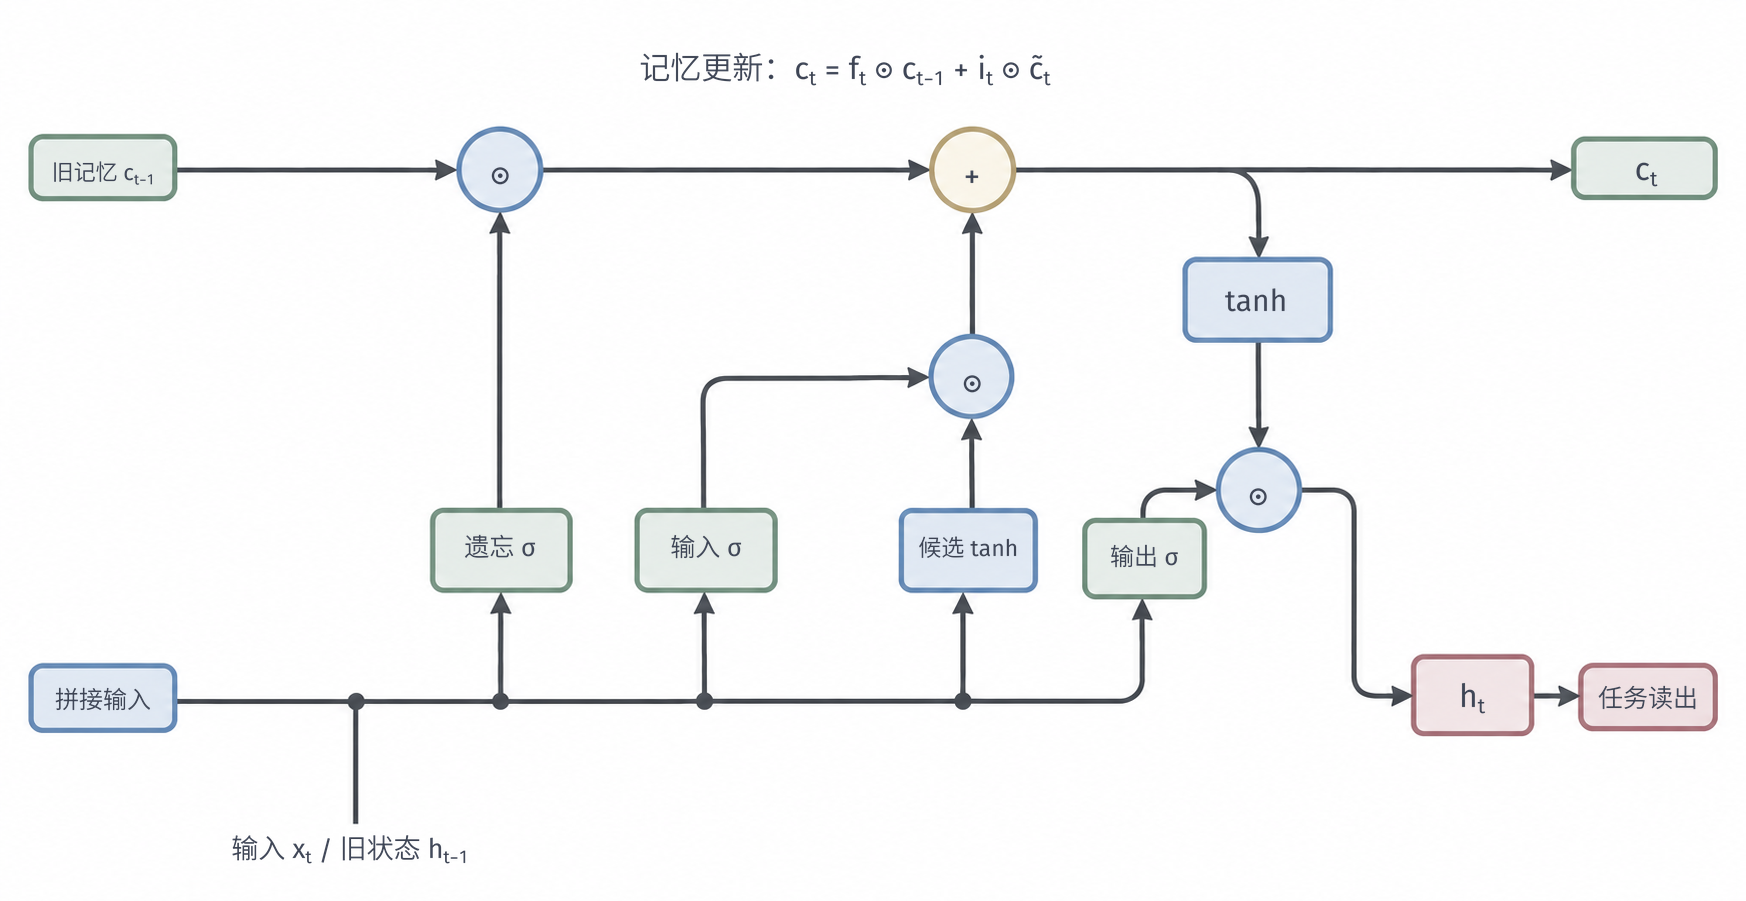
\includegraphics[width=147.828mm]{figures/05-neural-network-models/00-shared/generated/rnn-lstm-cell/figure.png}
  \caption{LSTM更新与任务读出。框外左侧为当前输入$\bm x_t$和旧状态$\bm h^{(t-1)},\bm c^{(t-1)}$，右侧为新状态和预测$\widehat{\bm y}_t=g(\bm V\bm h^{(t)}+\bm c)$。三个Sigmoid模块分别产生遗忘门、输入门和输出门，Tanh框产生候选记忆；圆形$\odot$与$+$分别表示逐元素乘法和相加。门值0阻断对应路径的信息，门值1让信息通过。}
  \label{fig:rnn-lstm-cell}
\end{figure*}
\FloatBarrier

如果暂把门与候选值看作已给定量，记忆路径对旧记忆的直接导数为$\operatorname{diag}(\bm{f}^{(t)})$。沿这条路径从$s$到$t$有
\begin{equation}
  \left.\frac{\partial\bm c^{(t)}}{\partial\bm c^{(s)}}\right|_{\mathrm{direct}}
    =\operatorname{diag}\!\left(\prod_{u=s+1}^{t}\bm f^{(u)}\right)\text{，}
  \label{eq:rnn-lstm-direct-memory}
\end{equation}
乘积按坐标进行。与普通RNN的$\bm D\bm W$相比，这条路径用可学习的保留率替代反复稠密混合；需要保存的坐标可令遗忘门接近1，并用较小输入门减少覆盖。这改变了式\eqref{eq:rnn-path-length-rate}中的逐步增益，通常没有缩短传播步数。但完整状态的Jacobian矩阵还包含$\bm h^{(t-1)}$影响各门和候选记忆的其他路径，直接路径与这些间接路径共同构成总导数。

\begin{example}[门值决定保留和写入]
  \label{ex:rnn-lstm-retention}
  考察一个记忆坐标，假设旧值为$2$，本步遗忘门为$0.9$、输入门为$0.2$、候选值为$0.5$。沿图~\ref{fig:rnn-lstm-cell}读取，左上$\odot$保留$0.9\times2=1.8$，中间$\odot$写入$0.2\times0.5=0.1$，再由上方$+$得到新记忆$1.9$。若输出门为$0.5$，右侧$\odot$产生隐藏输出$0.5\tanh(1.9)\approx0.478$，而非直接输出记忆值$1.9$。

  若之后100步不写入且遗忘门都为$0.99$，这份记忆沿直接路径的保留比例为$0.99^{100}\approx0.366$；门值为$0.9$时仅约$2.66\times10^{-5}$。加性记忆提供了可选择的保留率；小于1的门沿直接路径连续相乘，仍产生与距离有关的衰减。
\end{example}

图~\ref{fig:rnn-lstm-numerical-step}把例~\ref{ex:rnn-lstm-retention}扩展到两个记忆坐标。第一通道取较大的遗忘门和较小的输入门，主要保留旧值；第二通道反过来，主要写入候选值。$\odot$只在相同坐标之间相乘，不会把第一通道的门值作用到第二通道。两个通道可以采用不同的保留和写入比例。
\begin{figure*}[htbp]
  \centering
  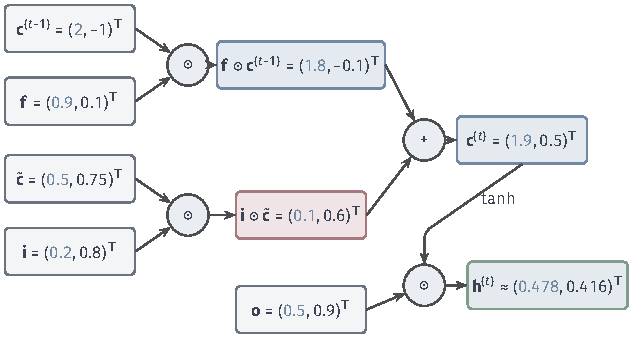
\includegraphics[width=107.107mm]{figures/05-neural-network-models/00-shared/tikz/rnn-lstm-numerical-step/figure.pdf}
  \caption{二维LSTM的一步数值走查。蓝色与深灰数字分别表示两个通道；保留分支计算$\bm f\odot\bm c^{(t-1)}$，写入分支计算$\bm i\odot\widetilde{\bm c}$，二者相加得到新记忆，再经$\bm o\odot\tanh(\bm c^{(t)})$得到隐藏状态。所有数值均由图内向量逐坐标计算，第二通道结果为$0.9\tanh(0.5)\approx0.416$。图中暂把门值和候选值视为已知，不展开它们的仿射计算。}
  \label{fig:rnn-lstm-numerical-step}
\end{figure*}
\FloatBarrier

记忆保持与信息读出仍要同时满足。即使直接路径没有明显衰减，过多写入也会覆盖证据；输出门较小或$\tanh(\bm c)$饱和时，任务损失仍可能难以作用于这段记忆。LSTM提供按任务选择保留、写入和读出的机制，完整梯度与预测表现需要对整个状态和读出分析。

训练仍使用BPTT，只需对记忆和隐藏两组状态共同求导。仅计上述单元，参数量为$4m(d+m+1)$，每步稠密仿射计算为$O(m(d+m))$，常数来自四组变换。增大初始遗忘门偏置可使初始保留比例较高，但门饱和也会减小自身的导数；这一选择需与长度和输入尺度匹配。

变体通常改变某条信息通路。\term{窥孔连接}（peephole connections）让门额外读取记忆坐标；耦合输入门与遗忘门可令$\bm{i}^{(t)}=\bm{1}-\bm{f}^{(t)}$，减少一组自由门。这些变体改变了门的依赖或自由度，适合程度需要在具体任务上比较\scite{greff2017}

% 避免两条完整变体引文在页底连续堆叠。
\Needspace{10\baselineskip}
若希望保留较宽记忆而减少循环映射成本，投影LSTM把记忆输出映射到更小的循环隐藏空间，使记忆宽度和循环宽度分开。投影把循环映射改为较小宽度，参数计数与前述等宽单元相应不同\scite{sak2014projection}

\subsection{GRU}
\label{sec:rnn-gru}

若希望简化状态管理，可以把记忆与隐藏输出合为一组变量。\term{门控循环单元}（gated recurrent unit, GRU）用更新门决定旧状态与候选状态的混合比例，用重置门控制候选计算怎样读取旧状态。这里采用Cho等原始形式的记号：更新门值越大，旧状态保留越多\scite{cho2014}

对同宽状态，方程为
\begin{equation}
  \begin{aligned}
    \bm{z}^{(t)}&=\operatorname{sigmoid}\!\left(
      \bm{U}_{\mathrm{z}}\bm{x}_t+\bm{W}_{\mathrm{z}}\bm{h}^{(t-1)}
      +\bm{b}_{\mathrm{z}}\right),\\
    \bm{r}^{(t)}&=\operatorname{sigmoid}\!\left(
      \bm{U}_{\mathrm{r}}\bm{x}_t+\bm{W}_{\mathrm{r}}\bm{h}^{(t-1)}
      +\bm{b}_{\mathrm{r}}\right),\\
    \widetilde{\bm{h}}^{(t)}&=\tanh\!\left(
      \bm{U}_{\mathrm{h}}\bm{x}_t
      +\bm{W}_{\mathrm{h}}(\bm{r}^{(t)}\odot\bm{h}^{(t-1)})
      +\bm{b}_{\mathrm{h}}\right),\\
    \bm{h}^{(t)}&=\bm{z}^{(t)}\odot\bm{h}^{(t-1)}
      +(\bm{1}-\bm{z}^{(t)})\odot\widetilde{\bm{h}}^{(t)}\text{。}
  \end{aligned}
  \label{eq:rnn-gru-update}
\end{equation}
每组$\bm{U}$、$\bm{W}$和偏置的形状与普通RNN相同。重置门接近零时，候选计算弱化旧状态；更新门接近1时，即使候选发生变化，输出也主要保留旧值。重置门调节候选读入的旧状态，更新门调节候选写入的比例，两者作用于不同计算位置。

图~\ref{fig:rnn-gru-cell}显示了候选分支和保留分支。单独看保留分支，其直接传播系数为$\bm{z}^{(t)}$；完整导数还包含门和候选的变化，与LSTM一样，直接分支之外的依赖也参与求导。

\begin{figure*}[htb]
  \centering
  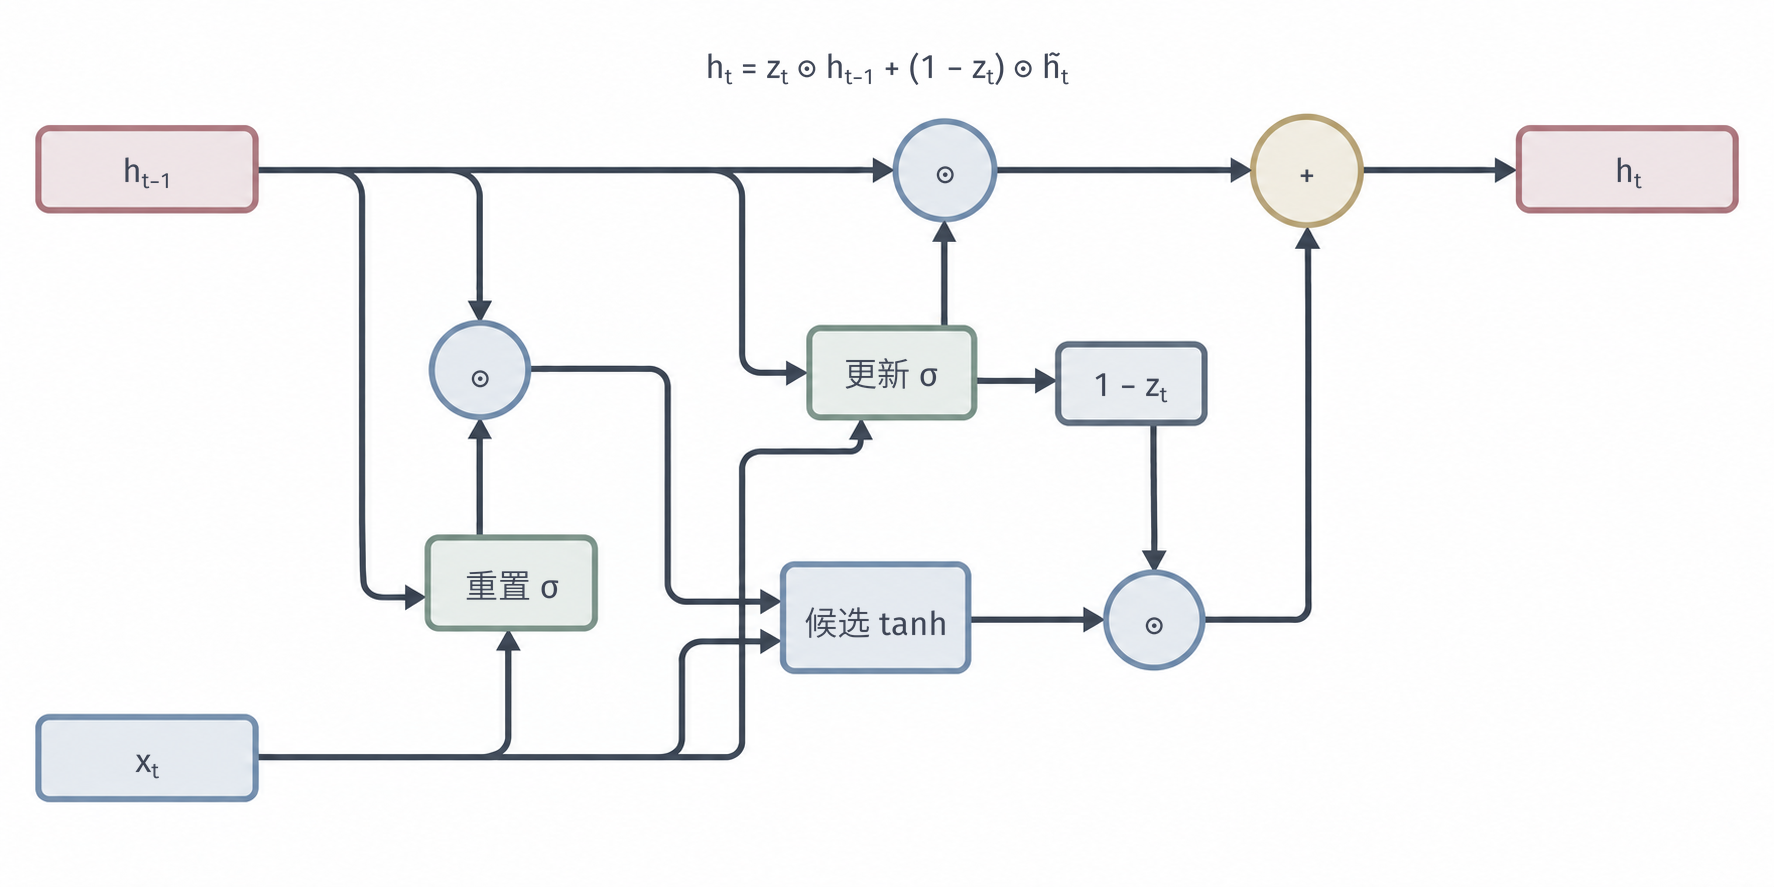
\includegraphics[width=150.199mm]{figures/05-neural-network-models/00-shared/generated/rnn-gru-cell/figure.png}
  \caption{GRU的状态更新。左侧输入为$\bm x_t$和旧状态$\bm h^{(t-1)}$，右侧输出为新状态。组合输入将当前输入与旧状态一并送入门和候选模块。重置门参与候选计算；顶部两个$\odot$框则显式形成$\bm z^{(t)}\odot\bm h^{(t-1)}$与$(\bm1-\bm z^{(t)})\odot\widetilde{\bm h}^{(t)}$，再相加得到新状态。任务预测还需在新状态之后另接读出。}
  \label{fig:rnn-gru-cell}
\end{figure*}
\FloatBarrier

GRU的长期保留对应更新门调节的直达分支。在需要延续记忆的坐标上，$\bm z^{(t)}$接近1时，状态更新接近复制旧值，沿保留路径的系数为各步$\bm z$的逐坐标乘积。候选分支的权重$\bm1-\bm z$同时较小，减少无关新输入覆盖已有状态。更新门接近0时则更多采用候选，允许网络改变当前记忆内容。

重置门的作用发生在候选计算中：它调节形成新候选时读取的旧状态量。重置门接近0、更新门接近1时，网络仍可以保留旧状态；更新门接近0时，即使重置门较大，旧信息也要通过非线性候选重新表达。没有独立记忆状态与输出门，还使GRU的保留内容和当前对外表示耦合得更紧。门接近恒等复制能改善一条梯度路径，门饱和、候选混合及读出仍可能限制长期学习。

在只用一组偏置的上述形式中，GRU单元参数量为$3m(d+m+1)$，少于等宽LSTM的四组变换，也只维护一个$m$维状态。代价是没有独立的记忆状态和输出门，存储与对外表示更直接地耦合。三组变换减少了等宽时的参数和状态存储，任务效果还取决于这种状态耦合是否适合目标；比较可在相近预算与预测条件下进行。

文献与软件还存在不同约定：有的把更新门定义为新候选的写入比例，有的把重置门放在$\bm{W}_{\mathrm{h}}\bm{h}^{(t-1)}$之后。前一种可通过交换$\bm{z}$与$1-\bm{z}$对应，后一种一般不能交换矩阵乘法与逐元素乘法，因此并非完全相同的更新。方程、偏置组数和门顺序共同确定具体GRU的计算与参数计数。

\FloatBarrier
\section{基于注意力的循环神经网络}
\label{sec:rnn-attention}

门控让网络\emph{更好地保存}信息，但前面的编码器—解码器结构还有一个结构性瓶颈：在式\eqref{eq:rnn-encoder-decoder}中，无论源序列多长，解码器都只能从编码器的\emph{同一个末状态}$\bm c_{\mathrm{enc}}=\bm h^{(T)}$读取信息。这等于要求网络把一整句话的所有细节压缩进一个固定维度的向量；输入越长，需要同时保存并区分的细节越多，这个瓶颈就越拥挤——即使编码器用的是LSTM也难以避免。

一个自然的想法是：\emph{不要只留摘要，把编码器每个位置的状态都保留下来，让解码器在生成每个词时“回头看”、按需取用}。翻译到当前词需要源句中的某个短语时，就给那个位置较高的权重；生成下一个词时再重新分配。这种根据当前需要动态加权读取一组表示的机制，就是\term{注意力机制}（attention mechanism）。它改变的是历史的\emph{读取方式}（而非保存方式），与门控（改变保存方式）正交，二者常一起使用。

\subsection{注意力机制}
\label{sec:rnn-attention-mechanism}

\term{注意力机制}（attention mechanism）根据当前计算需求给一组表示分配权重，再加权聚合：解码器需要的信息改变时，读取的上下文也随之改变。令编码器状态为$\bm{h}_1,\ldots,\bm{h}_T\in\mathbb{R}^{m}$，这里下标表示被保存的位置，$\bm{h}_t=\bm{h}^{(t)}$。对第$j$个解码步，给定查询$\bm{q}^{(j)}\in\mathbb{R}^{r}$，该向量承载本步解码需要读取哪些信息的线索，可以由解码状态或其变换产生。后面两种架构将确定查询采用旧状态还是本步新状态；此处先把查询视为已知，计算
\begin{equation}
  \begin{aligned}
    e_{j,t}&=a(\bm{q}^{(j)},\bm{h}_t),\\
    \alpha_{j,t}&=\frac{\exp(e_{j,t})}
       {\sum_{u=1}^{T}\exp(e_{j,u})},\\
    \bm{c}^{(j)}&=\sum_{t=1}^{T}\alpha_{j,t}\bm{h}_t\text{。}
  \end{aligned}
  \label{eq:rnn-attention}
\end{equation}
评分函数$a$比较查询与候选表示的相关程度。Softmax使权重非负且总和为1，$\bm{c}^{(j)}$是本步的动态上下文。归一化只在有效输入位置上进行，填充位置通过掩码排除。对很大的得分减去最大值再取指数，不改变权重，却可避免指数溢出。

评分可以通过非线性组合学习，也可以使用内积。\term{加性注意力}（additive attention）先把查询和编码状态投影到同一评分空间，再给出标量：
\begin{equation}
  e_{j,t}=\bm{v}_{\mathrm{a}}^{\top}\tanh\!\left(
     \bm{W}_{\mathrm{q}}\bm{q}^{(j)}
     +\bm{W}_{\mathrm{h}}\bm{h}_t+\bm{b}_{\mathrm{a}}\right)\text{。}
  \label{eq:rnn-additive-attention}
\end{equation}
设评分空间宽度为$a$，则$\bm{W}_{\mathrm{q}}\in\mathbb{R}^{a\times r}$、$\bm{W}_{\mathrm{h}}\in\mathbb{R}^{a\times m}$、$\bm{v}_{\mathrm{a}},\bm{b}_{\mathrm{a}}\in\mathbb{R}^{a}$。它允许查询和编码状态原本具有不同维度。

\term{点积注意力}（dot-product attention）直接用内积评分，在$r=m$时可取$e_{j,t}=\langle\bm{q}^{(j)},\bm{h}_t\rangle$；一般形式可取$e_{j,t}=(\bm{q}^{(j)})^{\top}\bm{W}_{\mathrm{a}}\bm{h}_t$，其中$\bm{W}_{\mathrm{a}}\in\mathbb{R}^{r\times m}$。点积形式便于批量矩阵计算，加性形式通过额外非线性改变评分函数，两者的适合程度仍由任务和宽度决定。Transformer章会继续讨论缩放、多头和位置编码，这里只需理解评分、归一化和聚合。

\begin{example}[权重与上下文]
  \label{ex:rnn-attention-context}
  假设本步对三个位置的得分为$0,\log2,0$，相应状态为$(1,0)^{\top}$、$(0,2)^{\top}$、$(1,1)^{\top}$。归一化权重为$(1/4,1/2,1/4)$，上下文为$(1/2,5/4)^{\top}$。第二个位置贡献较大，但上下文仍混合了三个状态；软聚合把多个状态的贡献相加，最终预测还取决于这些状态的内容及后续计算。
\end{example}

\subsection{网络结构}
\label{sec:rnn-attentive-architecture}

动态上下文可以参与解码状态更新，也可以在更新后参与输出。Bahdanau等的模型用此前解码状态查询编码表示，先形成$\bm{c}^{(j)}$，再计算本步状态：
\begin{equation}
  \begin{aligned}
    \bm{q}^{(j)}&=\bm{s}^{(j-1)},\\
    \bm{s}^{(j)}&=F_{\mathrm{dec}}\!\left(
      \bm{s}^{(j-1)},\bm{e}(y_{j-1}),\bm{c}^{(j)}\right),\\
    \bm{p}^{(j)}&=G\!\left(\bm{s}^{(j)},\bm{c}^{(j)},\bm{e}(y_{j-1})\right)\text{。}
  \end{aligned}
  \label{eq:rnn-bahdanau-order}
\end{equation}
$G$是输出概率映射，包含所需的可学习变换和归一化。编码器可以双向读取输入，使每个位置的表示同时包含前后上下文；编码器读取完整源输入，解码器生成时仍只使用此前目标\scite{bahdanau2015}

Luong等则先计算本步解码状态，再用该状态查询，形成融合后的输出表示：
\begin{equation}
  \begin{aligned}
    \bm{s}^{(j)}&=F_{\mathrm{dec}}\!\left(
      \bm{s}^{(j-1)},\bm{e}(y_{j-1})\right),\\
    \bm{q}^{(j)}&=\bm{s}^{(j)},\qquad
    \widetilde{\bm{s}}^{(j)}=
       \tanh\!\left(\bm{W}_{\mathrm{c}}[\bm{s}^{(j)};\bm{c}^{(j)}]\right),\\
    \bm{p}^{(j)}&=\operatorname{softmax}\!\left(
      \bm{V}_{\mathrm{a}}\widetilde{\bm{s}}^{(j)}+\bm{b}_{\mathrm{a}}\right)\text{。}
  \end{aligned}
  \label{eq:rnn-luong-order}
\end{equation}
其输入馈送变体还把前一步融合表示送入下一步解码。两个模型的关键区别之一是查询产生的时机和上下文进入的路径，若把当前状态查询放进式\eqref{eq:rnn-bahdanau-order}而保留其余依赖，查询与本步更新就互相等待；具体架构通过明确先后次序建立可执行的计算\scite{luong2015}

\term{全局注意力}（global attention）对全部有效输入位置评分，生成$S$个符号通常需要$ST$个位置对评分。\term{局部注意力}（local attention）只考虑某个位置附近的窗口，可固定窗口推进方式，也可由状态预测中心。窗口降低了读取范围与评分数量，但可能遗漏远处证据；可学习中心、连续位置权重和边界处理还需明确。局部方法预先限制本步评分的候选位置；全局权重集中则仍在完整位置集合上评分。

图~\ref{fig:rnn-attention-paths}采用先查询、后更新的组织方式。保存的编码状态建立了一条从输出直接读取早期位置的路径，减轻了所有细节只能经过编码末状态的限制。它同时需要保存整段编码表示，每个生成步还要执行读取，代价与固定状态读出不同。

\begin{figure*}[htb]
  \centering
  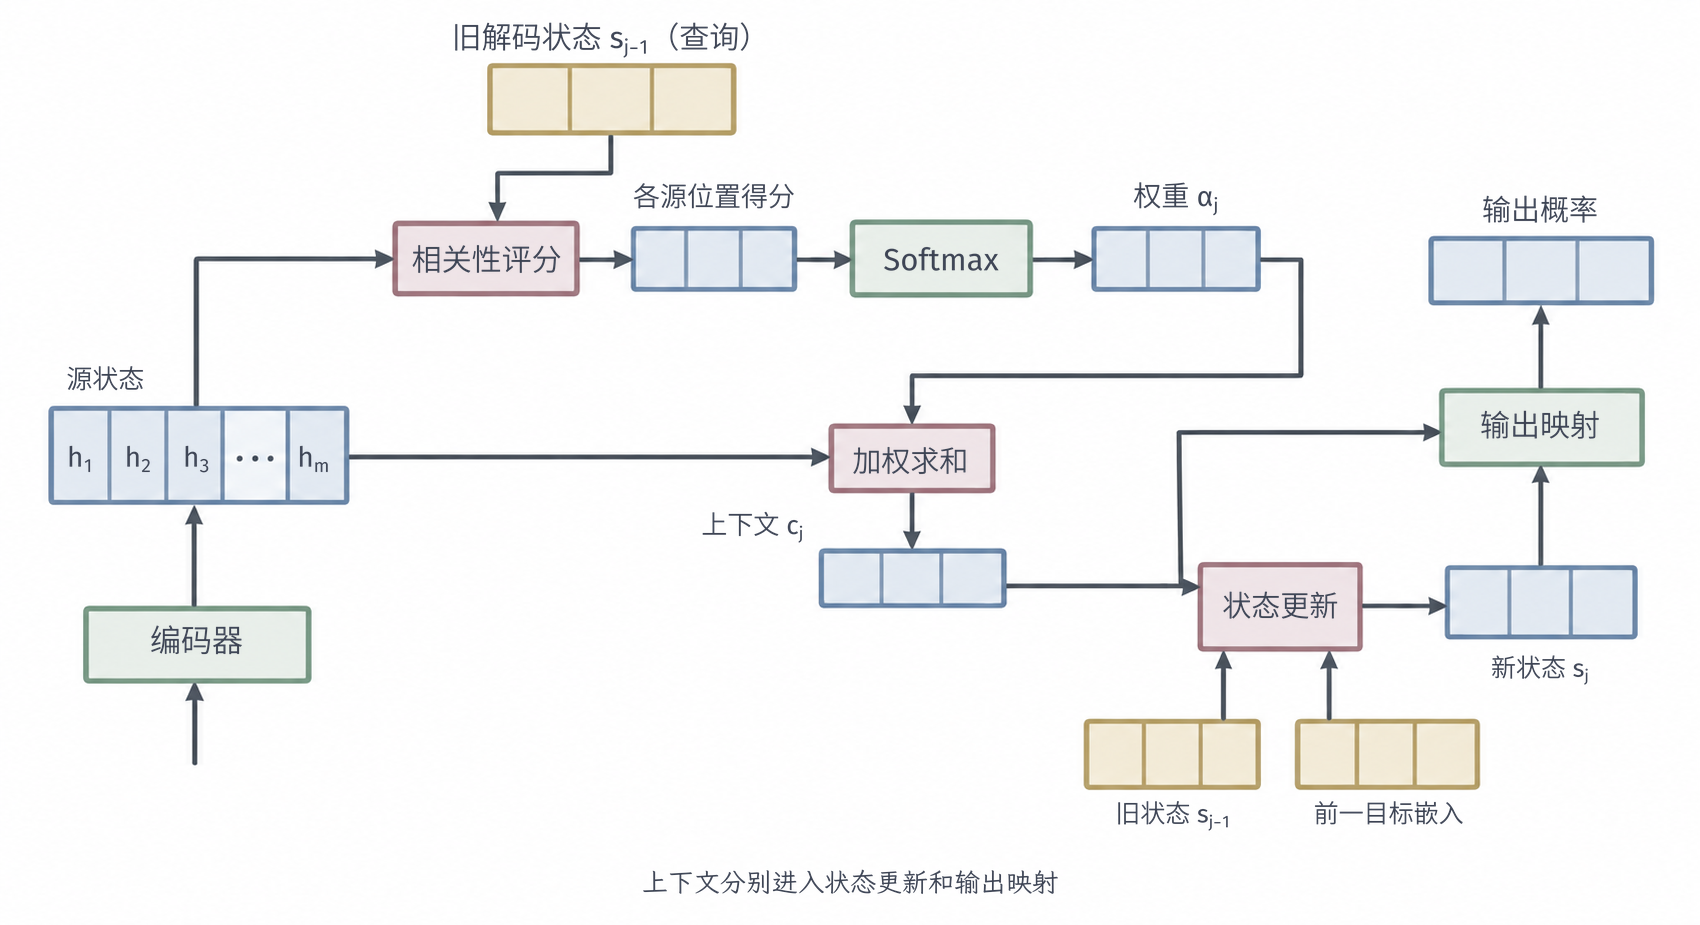
\includegraphics[width=143.933mm]{figures/05-neural-network-models/00-shared/generated/rnn-attention-paths/figure.png}
  \caption{带注意力的一个解码步。左侧为保存的编码状态$\bm h_{1:T}$、旧解码状态和此前目标的嵌入，右侧为新解码状态和输出概率。查询先用旧解码状态产生权重$\bm\alpha_j=(\alpha_{j,1},\ldots,\alpha_{j,T})$，上下文再进入更新与输出映射；输出映射还可读取目标嵌入。编码状态在各解码步重复读取，图中不重新执行编码器。}
  \label{fig:rnn-attention-paths}
\end{figure*}
\FloatBarrier


注意力对长期依赖的作用，可以从读取路径直接看出。暂固定本步评分和权重时，动态上下文对第$t$个编码状态的直接导数为
\begin{equation}
  \left.\frac{\partial\bm c^{(j)}}{\partial\bm h_t}\right|_{\bm\alpha_j\ \mathrm{fixed}}
       =\alpha_{j,t}\bm I\text{。}
  \label{eq:rnn-attention-direct-path}
\end{equation}
该分支从上下文直接到保存的表示，不再要求第$t$个状态经过其后全部编码状态才能被读取。权重若均匀，系数为$1/T$；若本步评分集中于相关位置，相应系数可以更大。这与普通时间链上的指数连乘具有不同的路径结构。

动态读取的对象是编码器已经形成的$\bm h_t$，其中保留了哪些历史仍由编码计算决定；评分过度分散或集中到无关位置时，相关证据的聚合贡献会减弱。保存各位置状态扩大了可访问范围，代价是随源长度增长的存储和读取。完整导数还包含评分随编码状态变化的分支，下一小节会把它与编码器、解码器的时间梯度合在一起。

\subsection{参数学习}
\label{sec:rnn-attention-learning}

编码器、评分函数、解码器和输出层可以按式\eqref{eq:rnn-sequence-likelihood}联合学习。软聚合可微，无需为每个目标另给一个位置标签。要理解注意力如何收到监督，暂固定查询并只看一个上下文节点。令$\bm{g}_{\mathrm{c}}^{(j)}=\partial L/\partial\bm{c}^{(j)}$，Softmax导数给出
\begin{equation}
  \frac{\partial L}{\partial e_{j,t}}
    =\alpha_{j,t}\left\langle
      \bm{g}_{\mathrm{c}}^{(j)},\bm{h}_t-\bm{c}^{(j)}\right\rangle\text{。}
  \label{eq:rnn-attention-score-gradient}
\end{equation}
其来源是$\partial\alpha_{j,u}/\partial e_{j,t}=\alpha_{j,u}(\mathbf{1}_{\{u=t\}}-\alpha_{j,t})$。增加某个得分会提高对应状态的相对权重，并降低其他权重；所以梯度比较的是该状态与当前平均上下文的差异，而不是仅看该状态的绝对值。

沿当前上下文节点反向计算时，链式法则把各个权重分量的变化相加：
\[
  \begin{aligned}
    \frac{\partial L}{\partial e_{j,t}}
      &=\sum_{u=1}^{T}
        \left\langle\bm g_{\mathrm c}^{(j)},\bm h_u\right\rangle
        \alpha_{j,u}(\mathbf{1}_{\{u=t\}}-\alpha_{j,t})\\
      &=\alpha_{j,t}\left(
        \left\langle\bm g_{\mathrm c}^{(j)},\bm h_t\right\rangle
        -\sum_{u=1}^{T}\alpha_{j,u}
         \left\langle\bm g_{\mathrm c}^{(j)},\bm h_u\right\rangle
        \right)\text{。}
  \end{aligned}
\]
求和项等于$\langle\bm g_{\mathrm c}^{(j)},\bm c^{(j)}\rangle$，再利用内积的线性便得到式\eqref{eq:rnn-attention-score-gradient}。这里仍只跟踪经过本步上下文的贡献；查询和时间依赖的其他路径随后再合入。

对编码状态还存在直接聚合贡献$\alpha_{j,t}\bm{g}_{\mathrm{c}}^{(j)}$，以及该状态改变评分产生的间接贡献。多个解码步的贡献相加后，再沿编码器的时间依赖回传；查询和解码状态也收到评分路径与输出路径的梯度。注意力缩短了部分信息与梯度路径，但编码器和解码器仍有循环依赖，权重过度集中或趋于零也可能削弱某些位置的监督。

\FloatBarrier
\section{状态空间模型}
\label{sec:rnn-state-space}

门控解决了“保存什么”，注意力解决了“读取什么”，但到2020年前后，经典RNN（含LSTM、GRU）仍有一个工程上的硬伤：它们的状态更新必须\emph{一步接一步串行}进行，第$t$步依赖第$t-1$步的结果，无法像卷积那样在一整段已知序列上大规模并行，这使得在现代并行硬件上训练超长序列很慢。状态空间模型（SSM）这条路线，正是从状态转移的\emph{代数形式}入手，试图让同一个序列模型能在两种计算方式之间自由切换：\emph{训练}时整段序列已知，就用可并行的卷积或扫描一次性处理；\emph{推理}时逐个生成，就退回成只维护定长状态的递推。此外，它还借鉴HiPPO为“状态应该保存历史的哪些信息”给出一个有数学依据的初始化。

先明确术语：这里的\term{状态空间模型}（state space model, SSM）专指用于神经序列网络的状态更新与读出模块；“状态空间模型”一词在控制论和概率建模中含义更广，本节不讨论随机状态估计的完整框架。本节的推进是：先建立线性状态更新的三种等价计算视角（递推、卷积、并行扫描），再讲HiPPO如何规定状态内容、S4如何让长卷积核的生成变得高效、Mamba如何让更新随输入内容变化，最后介绍RWKV的加权累积组织。

\subsection{状态空间表示与并行计算基础}
\label{sec:rnn-ssm-foundations}

先从连续时间的线性状态方程出发（这种形式便于用统一的参数控制不同分辨率，也直接对应控制论中的经典模型）。线性状态更新把旧状态和当前输入分别线性映射后相加，输出再读取新状态及当前输入。网络可以学习这些映射的矩阵参数，将系统的动态响应用于序列预测（历史累计作用参考\BookSectionRef{sec:signal-analysis-state-history-kernels}{卷2《数学准备：概率、因果与决策》第4章“动力系统”第4.2.1节“历史输入的累计作用”}，连续系统的离散计算参考\BookSectionRef{sec:dynamical-discretization-scan}{卷2《数学准备：概率、因果与决策》第4章“动力系统”第4.3.5节“离散化条件下的轨迹求解”}）。对连续输入$\bm{x}(\tau)\in\mathbb{R}^{d}$，表示为
\begin{equation}
  \frac{\mathrm{d}\bm{h}(\tau)}{\mathrm{d}\tau}
    =\bm{A}\bm{h}(\tau)+\bm{B}\bm{x}(\tau),
  \qquad
  \bm{y}(\tau)=\bm{C}\bm{h}(\tau)+\bm{D}\bm{x}(\tau)\text{。}
  \label{eq:rnn-continuous-ssm}
\end{equation}
其中$\bm{h}(\tau)\in\mathbb{R}^{m}$，$\bm{A}\in\mathbb{R}^{m\times m}$、$\bm{B}\in\mathbb{R}^{m\times d}$、$\bm{C}\in\mathbb{R}^{q\times m}$、$\bm{D}\in\mathbb{R}^{q\times d}$；$\bm{D}$给出当前输入直达输出的通路。$\tau$表示连续时间，避免与离散步数$t$混淆。此处先固定矩阵和步长，称为\term{线性时不变}（linear time-invariant, LTI）：叠加成立，转移规则也不随时间位置改变。

如果每个采样区间长$\Delta>0$且输入在区间内保持常值，解线性微分方程得到\term{零阶保持离散化}（zero-order hold discretization）：
\begin{equation}
  \begin{aligned}
    \overline{\bm{A}}&=\exp(\Delta\bm{A}),
    &\overline{\bm{B}}&=\int_0^{\Delta}\exp(u\bm{A})\bm{B}\,\mathrm{d}u,\\
    \bm{h}^{(t)}&=\overline{\bm{A}}\bm{h}^{(t-1)}
       +\overline{\bm{B}}\bm{x}_t,
    &\bm{y}_t&=\bm{C}\bm{h}^{(t)}+\bm{D}\bm{x}_t\text{。}
  \end{aligned}
  \label{eq:rnn-ssm-zoh}
\end{equation}
这里用当前输入先更新状态，再读取输出；离散状态记为当前保持区间的末状态，直接项也使用该区间的输入。$\exp$是矩阵指数。$\bm{A}$可逆时，积分可写为$\bm{A}^{-1}(\exp(\Delta\bm{A})-\bm{I})\bm{B}$；积分形式在不可逆时仍有意义。网络也可以直接学习离散矩阵，不必总从连续方程出发。

在零初始状态、固定离散矩阵下，反复代入递推可得
\begin{equation}
  \begin{aligned}
    \bm{h}^{(t)}&=\sum_{u=1}^{t}
       \overline{\bm{A}}^{t-u}\overline{\bm{B}}\bm{x}_u,\\
    \bm{y}_t&=\sum_{k=0}^{t-1}\bm{K}_k\bm{x}_{t-k}
       +\bm{D}\bm{x}_t,\qquad
    \bm{K}_k=\bm{C}\overline{\bm{A}}^k\overline{\bm{B}}\text{。}
  \end{aligned}
  \label{eq:rnn-ssm-convolution}
\end{equation}
$\bm{K}_k\in\mathbb{R}^{q\times d}$是滞后$k$步的响应：它刻画“$k$步以前的输入对当前输出还有多大、以什么模式的影响”。这个展开式是理解全节的枢纽，它一举给出了三种计算视角：
\begin{itemize}
  \item \emph{递推视角}：逐时刻更新定长状态$\bm h^{(t)}$，只需保存当前状态，适合逐步生成；
  \item \emph{卷积视角}：输出是历史输入与固定核$\bm K_k$的加权和，可以用卷积（进而用FFT）对整段序列并行计算；
  \item \emph{并行扫描视角}：当各步的线性变换已知时，可用满足结合律的有序复合把前缀状态并行算出（见下文）。
\end{itemize}
三种视角描述的是\emph{同一个线性模型}，区别只在计算组织方式。核只依赖滞后$k$而不依赖绝对位置，所以这是一个因果卷积；非零初态还会增加$\bm{C}\overline{\bm{A}}^t\bm{h}^{(0)}$；一旦系数随时间或输入变化，就一般不能再并入同一个固定卷积核（这正是后面Mamba要单独处理的地方）。

并行计算还有另一条基础。对已知的仿射更新$\bm{h}^{(t)}=\bm{A}_t\bm{h}^{(t-1)}+\bm{b}_t$，用二元组$(\bm{A}_t,\bm{b}_t)$表示一步变换。先执行$P$再执行$Q$的组合定义为
\begin{equation}
  (\bm{A}_Q,\bm{b}_Q)\circ(\bm{A}_P,\bm{b}_P)
   =(\bm{A}_Q\bm{A}_P,
      \bm{A}_Q\bm{b}_P+\bm{b}_Q)\text{。}
  \label{eq:rnn-affine-composition}
\end{equation}
这一有序复合满足结合律，因此可以进行\term{关联扫描}（associative scan）：
先组合连续片段，再恢复所有前缀（复合规则参考\BookEquationRef{eq:dynamical-affine-composition}{卷2《数学准备：概率、因果与决策》第4章“动力系统”第4.3.1.2节“基于并行扫描的仿射轨迹求解”}）。各步系数提前已知时，组合可先处理连续片段。依赖尚未算出旧状态的非线性更新，则需先获得相应状态才能确定下一变换。图~\ref{fig:rnn-scan}示意这一计算组织。

\begin{figure}[htb]
  \centering
  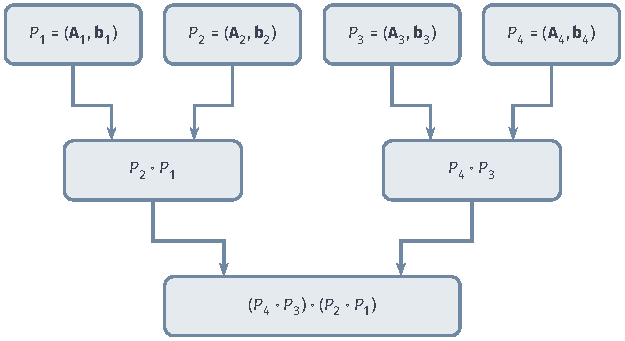
\includegraphics[width=105.791mm]{figures/05-neural-network-models/00-shared/tikz/rnn-scan/figure.pdf}
  \caption{仿射状态更新的有序组合。四个单步变换先组成两个连续片段，再组成整段；$Q\circ P$表示先执行$P$再执行$Q$。平衡组合树展示的是扫描中的汇总阶段，完整前缀扫描还要把此前片段的结果传给各位置，才能得到每步状态。树形计算可缩短依赖深度，但不改变输入顺序。}
  \label{fig:rnn-scan}
\end{figure}
\FloatBarrier

对逐坐标仿射更新，工作高效的扫描可用$O(Tm)$总运算量和$O(\log T)$组合深度得到前缀；稠密矩阵组合还要执行矩阵乘法，成本随状态宽度另行增加。普通RNN的非线性组合也通常无法保持固定大小、便于计算的仿射表示。可并行的条件是各步系数可提前取得、组合闭合且足够便宜；若系数必须由尚未计算的旧状态产生，就不能直接预先扫描。

\begin{example}[同一状态模型的递推与卷积]
  \label{ex:rnn-ssm-equivalence}
  取标量更新$h^{(t)}=\tfrac12 h^{(t-1)}+x_t$、$y_t=h^{(t)}$、$h^{(0)}=0$，输入为$(1,2,0)$。递推得到$(1,5/2,5/4)$。卷积核为$(1,1/2,1/4,\ldots)$，故第三步输出为$0+\tfrac12\times2+\tfrac14\times1=5/4$。整段训练可以按卷积组织，逐步预测可以按状态组织；相同输出来自相同模型的代数等价，而不是两套分别训练的参数。
\end{example}

\subsection{HiPPO}
\label{sec:rnn-hippo}

前面的线性框架解决了“怎么算”，却没有回答一个更根本的问题：状态里到底\emph{该存什么}，才能用有限的$m$个数最好地概括整段历史？随意选一个状态矩阵并不能保证它保留了远期信息。\term{高阶多项式投影}（high-order polynomial projection operators, HiPPO）把“记忆”显式定义成一个在线近似问题：\emph{用$m$个随时间更新的系数，去逼近到目前为止的整段历史函数，使加权平方误差最小}。相比只存一个滑动平均，多个基函数系数可以分别刻画历史的平均水平、变化趋势、曲率等不同形态\scite{gu2020hippo}。这个投影思路给出的更新矩阵，后来成为S4初始化状态动态的依据。

\subsubsection{投影系数保存什么}
\label{sec:rnn-hippo-memory}

设标量历史信号为$f(u)$，在当前时刻$\tau$选定历史权重测度$\mu_\tau$和相应正交归一基$p_0(u;\tau),\ldots,p_{m-1}(u;\tau)$。在该测度下平方可积时，投影系数与近似信号为
\begin{equation}
  c_i(\tau)=\int f(u)p_i(u;\tau)\,\mathrm{d}\mu_\tau(u),
  \qquad
  \widehat f_\tau(u)=\sum_{i=0}^{m-1}c_i(\tau)p_i(u;\tau)\text{。}
  \label{eq:rnn-hippo-projection}
\end{equation}
它在所选$m$维基函数空间中最小化加权平方误差。状态记录这组基函数系数；每个系数汇集一个历史形状的影响，权重与有限基函数数目共同决定可保留的细节。

\subsubsection{在线更新与网络组织}
\label{sec:rnn-hippo-architecture}

例如缩放Legendre版本在$[0,\tau]$上采用均匀权重，将整个历史区间缩放到固定区间上的Legendre多项式。
这里采用归一化的均匀测度，使整个区间的总权重为1。前两个基函数具体为
\[
  \begin{aligned}
    \mathrm d\mu_\tau(u)
      &=\frac{\mathbf{1}_{[0,\tau]}(u)}{\tau}\,\mathrm du,\\
    p_0(u;\tau)&=1,\\
    p_1(u;\tau)&=\sqrt3\left(\frac{2u}{\tau}-1\right)\text{。}
  \end{aligned}
\]
更高阶可取$p_i(u;\tau)=\sqrt{2i+1}\,P_i(2u/\tau-1)$，其中$P_i$是$[-1,1]$上满足$P_i(1)=1$的Legendre多项式。换元$z=2u/\tau-1$后，测度变为$\mathrm dz/2$；Legendre多项式在该测度下的平方积分为$1/(2i+1)$，因此因子$\sqrt{2i+1}$把每个基的范数归一到1，不同阶仍正交。

投影定义给出了任一时刻的系数，在线更新还要回答：区间从$[0,\tau]$略微延长后，怎样只用旧系数和新端点值更新它们。我们先取$m=2$看清这一步。为直接使用通常的Leibniz积分求导法则，以下走查暂设$f$连续，并始终取$\tau>0$；连续性是此处求导采用的条件，比定义投影时的平方可积条件更强。将前两个基代入投影式，有
\[
  \begin{aligned}
    c_0(\tau)&=\frac1\tau\int_0^\tau f(u)\,\mathrm du,\\
    c_1(\tau)&=\frac{\sqrt3}{\tau}
      \int_0^\tau f(u)\left(\frac{2u}{\tau}-1\right)\,\mathrm du\text{。}
  \end{aligned}
\]
求导时有三种变化需要分开：积分区间增加了新端点，归一化权重$1/\tau$改变，基函数也随区间长度改变。对$i=0,1$，把这三项分别写出便是
\[
  \begin{aligned}
    \frac{\mathrm dc_i}{\mathrm d\tau}
      &=\frac{f(\tau)p_i(\tau;\tau)}{\tau}
        -\frac{c_i(\tau)}{\tau}\\
      &\quad+\frac1\tau\int_0^\tau
        f(u)\frac{\partial p_i(u;\tau)}{\partial\tau}\,\mathrm du\text{。}
  \end{aligned}
\]
$p_0$不随$\tau$变化，而$p_1(\tau;\tau)=\sqrt3$、$\partial p_1(u;\tau)/\partial\tau=-2\sqrt3\,u/\tau^2$，所以
\[
  \begin{aligned}
    \frac{\mathrm dc_0}{\mathrm d\tau}
      &=\frac{f(\tau)-c_0(\tau)}{\tau},\\
    \frac{\mathrm dc_1}{\mathrm d\tau}
      &=\frac{\sqrt3 f(\tau)-c_1(\tau)}{\tau}
        -\frac{2\sqrt3}{\tau^3}\int_0^\tau u f(u)\,\mathrm du\text{。}
  \end{aligned}
\]
第二行还含一阶历史矩；但它已经包含在$c_0,c_1$中，无需保存整个历史来重新积分。由$c_1$的积分表达式整理可得
\[
  \begin{aligned}
    c_1(\tau)
      &=\frac{2\sqrt3}{\tau^2}\int_0^\tau u f(u)\,\mathrm du
        -\sqrt3 c_0(\tau),\\
    \frac{2\sqrt3}{\tau^3}\int_0^\tau u f(u)\,\mathrm du
      &=\frac{c_1(\tau)+\sqrt3 c_0(\tau)}{\tau}\text{。}
  \end{aligned}
\]
代回后，两个系数的更新闭合为
\[
  \begin{aligned}
    \frac{\mathrm dc_0}{\mathrm d\tau}
      &=\frac{f(\tau)-c_0(\tau)}{\tau},\\
    \frac{\mathrm dc_1}{\mathrm d\tau}
      &=\frac{\sqrt3 f(\tau)-\sqrt3 c_0(\tau)-2c_1(\tau)}{\tau}\text{。}
  \end{aligned}
\]
新端点提供当前输入项，权重和基的变化共同产生旧系数项；其中$c_0$进入$c_1$的更新，正是移动基带来的系数耦合。更高阶也可用基函数关系把求导后出现的历史矩写回已有系数，得到下面的一般矩阵形式。

使用从零开始的$i,j\in\{0,\ldots,m-1\}$，其连续系数更新可写为
\begin{equation}
  \begin{aligned}
    \frac{\mathrm{d}\bm{c}(\tau)}{\mathrm{d}\tau}
      &=-\frac{1}{\tau}\bm{H}\bm{c}(\tau)
        +\frac{1}{\tau}\bm{b}f(\tau),\qquad \tau>0,\\
    H_{i,j}&=
      \begin{cases}
        \sqrt{(2i+1)(2j+1)},&i>j,\\
        i+1,&i=j,\\
        0,&i<j,
      \end{cases}
      \qquad b_i=\sqrt{2i+1}\text{。}
  \end{aligned}
  \label{eq:rnn-hippo-legs}
\end{equation}
随时间变化的$1/\tau$反映历史区间不断扩张，更新矩阵也随当前时间改变。$m=1$时，$c_0$是整个区间的均值，其导数为$(f(\tau)-c_0(\tau))/\tau$，这给出了系数更新的直观核验。离散实现需选择初始化和离散化，不能在$\tau=0$直接代入。

测度决定“哪些历史值得近似”：固定窗口强调近期区间，指数权重弱化久远输入，随时间扩张的均匀区间覆盖全部过去，但固定阶数的分辨率会受到区间增长影响。HiPPO提供状态构造原则和相应结构矩阵，完整预测网络仍需要输入变换、读出及学习目标。可以固定投影动态、学习前后变换，也可以以结构矩阵初始化后再调整；后者需要重新检查状态是否仍满足原来的投影含义。投影误差的性质不能直接代替任务泛化误差。


图~\ref{fig:rnn-hippo}展示了一种把投影记忆接入任务网络的方式。实际观测可先经过可学习映射形成$f(\tau)$；投影更新维护系数，任务读出利用系数产生预测。若输入有多个特征，可以为各通道分别维护一组系数，再混合通道。重构历史使用已选定的基函数，任务读出则由监督目标决定，两者用途不同。
\begin{figure}[htb]
  \centering
  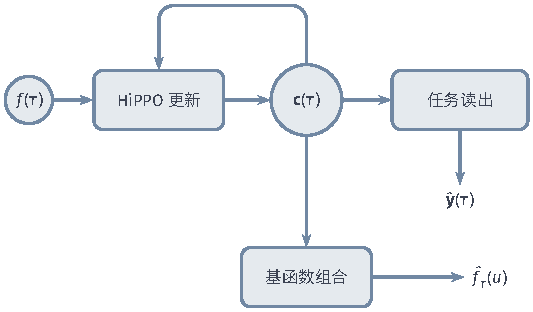
\includegraphics[width=90.293mm]{figures/05-neural-network-models/00-shared/tikz/rnn-hippo/figure.pdf}
  \caption{HiPPO投影记忆与任务网络的一种组合。反馈维护系数状态，读出产生任务预测；下方将同一系数与基函数组合，近似重构历史信号。HiPPO本身规定记忆表示及更新，图中的任务读出与输入特征映射可另行学习，并非唯一的HiPPO网络架构。}
  \label{fig:rnn-hippo}
\end{figure}
\FloatBarrier

若投影动态固定，任务损失训练输入映射和读出；输入映射可学习时，梯度仍需经过投影递推回到此前输入特征。若进一步训练投影矩阵，模型获得调整动态的自由，也放松了投影所规定的约束。固定投影动态维持了原来的投影约束，训练矩阵则让任务调整状态响应；参数范围决定当前模型保留哪种投影含义。

\subsubsection{历史覆盖与长期依赖的边界}
\label{sec:rnn-hippo-long-memory}

LegS把全部过去放进随时间扩张的区间，没有用一个固定窗口把早期输入直接删除。最低阶系数是均值：在$[0,\tau]$上，$c_0(\tau)=\tau^{-1}\int_0^\tau f(u)\,\mathrm du$。时刻$u$附近面积为$\varepsilon$的窄脉冲，对这个均值的贡献约为$\varepsilon/\tau$，随当前时刻按倒数减弱，而不是按已经经过的更新步数以固定比例反复衰减。

这个性质也可从状态更新看出。对$0<\sigma<\tau$，将$[\sigma,\tau]$间的输入固定，初始系数扰动满足
\begin{equation}
  \delta\bm c(\tau)
    =\exp\!\left[-\bm H\log(\tau/\sigma)\right]\delta\bm c(\sigma)\text{。}
  \label{eq:rnn-hippo-time-ratio}
\end{equation}
因为此区间的齐次更新是$\delta\dot{\bm c}=-\bm H\delta\bm c/\tau$，积分变量是$\log\tau$。与固定矩阵的$\exp(\bm A(\tau-\sigma))$相比，LegS按时间比值组织保留；最低阶模式的系数为$\sigma/\tau$。完整状态传播还包含其他模式及范数常数，任务梯度另经过输入映射和读出；最低阶模式只展示了时间比值的一个保留尺度。

前面用前两个基函数推得了在线更新；下面把同一组系数带回重构式，检验这份有限记忆怎样恢复历史的水平和趋势。

多个系数提供的不是多个历史位置，而是多个形状特征。取$p_0=1$、$p_1=\sqrt3(2u/\tau-1)$，对线性历史$f(u)=a+bu$，两个系数为
\begin{equation}
  c_0=a+\frac{b\tau}{2},\qquad c_1=\frac{b\tau}{2\sqrt3}\text{。}
  \label{eq:rnn-hippo-linear-example}
\end{equation}
代回基函数组合即可精确恢复这条线性函数：第一个系数保存水平，第二个补上趋势。若历史含有很多窄尖峰，两个系数便不足以定位每个尖峰；提高阶数增加分辨能力，也增加状态与计算成本。

因此，HiPPO把长期记忆转为有明确误差准则的在线压缩。它适合考察较长区间上的形状和趋势，固定阶数、有限精度、所选测度与信号变化共同限制可恢复细节。模型若需要精确取回任意久远符号，还需检验相应信息在投影后是否可区分；任务网络的非线性与读出同样可能带来额外学习困难。

\subsection{S4}
\label{sec:rnn-s4}

HiPPO给了一个有依据的状态矩阵，但直接拿来训练仍有两个工程障碍：一是状态矩阵是稠密的$m\times m$矩阵，逐步递推每步都要做$O(m^2)$的矩阵乘法，状态一宽就很贵；二是想用卷积视角并行训练时，需要生成长度为$T$的卷积核$\bm K_k=\bm C\overline{\bm A}^k\overline{\bm B}$，而稠密矩阵反复相乘、再加上HiPPO矩阵直接对角化的数值不稳定，使这个核难以快速且稳定地求得。\term{结构化状态空间序列模型}（structured state space sequence model, S4）的核心贡献，就是找到状态矩阵的一种特殊数学分解（对角加低秩），使得递推、卷积核生成都能在近线性的代价下稳定进行\scite{gu2022s4}。

这里的S4状态模块采用不随时间位置改变的连续矩阵$\bm A$，以保持前面卷积表达所必需的线性时不变条件。它借用HiPPO的结构矩阵和初始化思想；注意前面LegS的$-\bm H/\tau$仍随历史区间扩展而改变，不能直接把那条时变投影更新当作此处的固定动态。

\subsubsection{结构矩阵与核生成}
\label{sec:rnn-s4-structure}

我们以刚才的$\bm H$为例，追踪结构分解与坐标变换怎样相接。取固定矩阵$\bm A_0=-\bm H\in\mathbb R^{m\times m}$，另定义实向量$\bm p\in\mathbb R^m$，其分量为$(\bm p)_i=\sqrt{(2i+1)/2}$，下标仍从0开始。这里$\bm p$用于分解矩阵，与前面随$u$变化的多项式基$p_i(u;\tau)$是不同对象。补上一个秩一矩阵后，得到
\[
  \begin{aligned}
    \bm N&=\bm A_0+\bm p\bm p^{\top}
      =-\frac12\bm I+\bm S,\\
    S_{i,j}&=
      \begin{cases}
        -\tfrac12\sqrt{(2i+1)(2j+1)},&i>j,\\
        0,&i=j,\\
        \tfrac12\sqrt{(2i+1)(2j+1)},&i<j\text{。}
      \end{cases}
  \end{aligned}
\]
对角线上$-(i+1)+(2i+1)/2=-1/2$，非对角元则成对反号，因此$\bm S^{\top}=-\bm S$。于是$\bm N\bm N^*=\bm N^*\bm N=\bm I/4-\bm S^2$，$\bm N$是正规矩阵，可以用酉矩阵$\bm V\in\mathbb C^{m\times m}$对角化为$\bm N=\bm V\bm\Lambda\bm V^*$，其中$\bm V^*\bm V=\bm I$。这一步对角化的是补正后的$\bm N$，原来的状态矩阵仍为$\bm A_0=\bm N-\bm p\bm p^{\top}$。

在连续模型$\dot{\bm h}=\bm A_0\bm h+\bm B\bm x$、$\bm y=\bm C\bm h+\bm D\bm x$中，将同一状态改用坐标$\bm h'=\bm V^*\bm h$表示，并同步变换输入、输出映射：
\[
  \begin{aligned}
    \bm A'&=\bm V^*\bm A_0\bm V
      =\bm\Lambda-(\bm V^*\bm p)(\bm V^*\bm p)^*,\\
    \bm B'&=\bm V^*\bm B,\qquad
    \bm C'=\bm C\bm V\text{。}
  \end{aligned}
\]
由$\bm h=\bm V\bm h'$代回，得到$\dot{\bm h}'=\bm A'\bm h'+\bm B'\bm x$和$\bm y=\bm C'\bm h'+\bm D\bm x$；因此改变的是状态坐标，输入到输出的映射保持不变，直达项$\bm D$也不变。初态同样需变为$\bm h'(0)=\bm V^*\bm h(0)$。原来稠密的正规部分现在只需对角矩阵$\bm\Lambda$表示，余下两向量的外积秩至多为1；“低秩”在这里表示只用少数方向修正对角动态，因此可以用少量列向量保存这项修正。

这个例子在复坐标中的两个低秩因子都为$\bm V^*\bm p\in\mathbb C^{m\times1}$。原模型为实数时，可将复数谱和相应系数按共轭对组织，中间复数项组合后仍给出原来的实输出；在复坐标中直接学习参数时，也需保持相应的共轭配对或采用等价的实数表示。下面省去新坐标的撇号，并用$\bm P,\bm Q$允许秩为$r$的修正。

其关键结构之一是\term{对角加低秩}（diagonal plus low-rank, DPLR）：在合适的复数坐标系中写为
\begin{equation}
  \bm{A}=\bm{\Lambda}-\bm{P}\bm{Q}^{*}\text{，}
  \label{eq:rnn-s4-dplr}
\end{equation}
其中$\bm{\Lambda}\in\mathbb{C}^{m\times m}$是对角矩阵，$\bm{P},\bm{Q}\in\mathbb{C}^{m\times r}$，秩$r$较小，$*$表示共轭转置。这个坐标系来自正规矩阵加低秩结构的酉变换；正规矩阵$\bm{N}$满足$\bm{N}\bm{N}^{*}=\bm{N}^{*}\bm{N}$，其酉对角化避免任意病态基变换，加入低秩项后的$\bm{A}$则不必正规。输入和输出映射也随坐标一起变换，实际输出可通过共轭配对保持实数。

前面的零阶保持规则在输入区间保持常值时精确积分连续动态。这里改用另一种离散化：在一个长度为$\Delta$的区间内，以首末状态的平均值近似状态项的积分，输入仍取本区间的常值$\bm x_t$，即
\[
  \bm h^{(t)}-\bm h^{(t-1)}
    \approx\frac{\Delta}{2}\bm A
       \left(\bm h^{(t)}+\bm h^{(t-1)}\right)
       +\Delta\bm B\bm x_t\text{。}
\]
把这条梯形近似作为离散更新的定义，再将含新状态的项移到左侧，可得精确的代数关系
\[
  \left(\bm I-\frac{\Delta}{2}\bm A\right)\bm h^{(t)}
    =\left(\bm I+\frac{\Delta}{2}\bm A\right)\bm h^{(t-1)}
       +\Delta\bm B\bm x_t\text{。}
\]
当左侧矩阵可逆时，左乘其逆即可得到下面的状态转移与写入矩阵。这种有理矩阵形式把所需计算转为线性矩阵的求逆作用，便于继续使用对角加低秩结构。

S4采用的双线性离散化为
\begin{equation}
  \begin{aligned}
    \overline{\bm{A}}&=
      (\bm{I}-\tfrac{\Delta}{2}\bm{A})^{-1}
      (\bm{I}+\tfrac{\Delta}{2}\bm{A}),\\
    \overline{\bm{B}}&=
      (\bm{I}-\tfrac{\Delta}{2}\bm{A})^{-1}\Delta\bm{B}\text{，}
  \end{aligned}
  \label{eq:rnn-s4-bilinear}
\end{equation}
需保证逆矩阵存在。DPLR形式使相关逆矩阵作用可以通过对角运算和低秩修正计算；固定秩时，一步递推可达到$O(m)$量级，而不是稠密状态转移的$O(m^2)$。

两种离散化在有限步长下一般给出不同参数。例如对零输入的标量衰减$A=-1$，取$\Delta=1$，零阶保持得到$\overline A=e^{-1}\approx0.368$，双线性规则则得到$\overline A=(1-1/2)/(1+1/2)=1/3$。两者都描述衰减，但只有前者在这里等于该保持区间的精确连续解；后续的递推、卷积和核生成必须使用各自离散规则给出的同一套参数。

核生成也利用这套结构。计算路线是先在$T$个单位根处求一个有限多项式的值，再用逆DFT恢复它的$T$个系数；这些系数就是所需的卷积核。把长度为$T$的核视为一个有限多项式，用几何和恒等式可写为
\begin{equation}
  \begin{aligned}
    \bm{G}_T(z)&=\sum_{k=0}^{T-1}\bm{K}_k z^k\\
      &=\bm{C}\left[\bm{I}-(z\overline{\bm{A}})^T\right]
         (\bm{I}-z\overline{\bm{A}})^{-1}\overline{\bm{B}}\text{，}
  \end{aligned}
  \label{eq:rnn-s4-generating-function}
\end{equation}
第二行适用于所写逆矩阵存在时，$T$表示有限核长度，矩阵上的$T$是幂次而非转置。要看清这个逆怎样利用DPLR结构，下面固定单输入单输出情形，记$\bm B=\bm b$、$\bm C=\bm c^*$，其中$\bm b,\bm c\in\mathbb C^m$；此时$\bm G_T$退化为标量多项式$G_T$，低秩$r$不随$m,T$增长。

由双线性离散化，
\[
  \bm I-z\overline{\bm A}
    =(\bm I-\tfrac{\Delta}{2}\bm A)^{-1}
      \left[(1-z)\bm I-\frac{\Delta}{2}(1+z)\bm A\right]\text{。}
\]
对$z\neq-1$，提出方括号中的系数，可将离散逆矩阵作用改写为
\begin{equation}
  \begin{aligned}
    \xi(z)&=\frac{2}{\Delta}\frac{1-z}{1+z},\\
    (\bm I-z\overline{\bm A})^{-1}\overline{\bm b}
      &=\frac{2}{1+z}(\xi(z)\bm I-\bm A)^{-1}\bm b\text{。}
  \end{aligned}
  \label{eq:rnn-s4-resolvent}
\end{equation}
其中$\overline{\bm b}=(\bm I-\Delta\bm A/2)^{-1}\Delta\bm b$。右侧的$(\xi\bm I-\bm A)^{-1}$称为预解矩阵（resolvent）。双线性变换把离散频率点$z$转为连续状态矩阵的频率变量$\xi$，上式仍以相关逆存在为前提。

核只保留有限长度，因此求值还带有截断因子。在$T$个单位根
$z_\ell=\exp(-2\pi\mathrm i\ell/T)$、$\ell=0,\ldots,T-1$上，$\mathrm i$为虚数单位，$z_\ell^T=1$，因此可以共用修正后的输出行
\begin{equation}
  \bm c_T^*=\bm c^*(\bm I-\overline{\bm A}^{T})\text{。}
  \label{eq:rnn-s4-finite-readout}
\end{equation}
代入式\eqref{eq:rnn-s4-generating-function}与式\eqref{eq:rnn-s4-resolvent}，对$z_\ell\neq-1$得到
\begin{equation}
  G_T(z_\ell)=\frac{2}{1+z_\ell}
    \bm c_T^*(\xi(z_\ell)\bm I-\bm A)^{-1}\bm b\text{。}
  \label{eq:rnn-s4-root-evaluation}
\end{equation}
这里利用$z^T=1$才把修正行统一为$\bm c_T^*$；一般$z$处仍须保留$\bm I-(z\overline{\bm A})^T$，修正项与$\bm I-\overline{\bm A}^T$在一般求值点上不同。

现在代入$\bm A=\bm\Lambda-\bm P\bm Q^*$。记$\lambda_j$为$\bm\Lambda$的第$j$个对角元素，并令
\[
  \bm R_\xi=(\xi\bm I-\bm\Lambda)^{-1}
    =\operatorname{diag}\!\left(
       \frac1{\xi-\lambda_1},\ldots,\frac1{\xi-\lambda_m}\right)\text{。}
\]
Woodbury恒等式把原来的$m\times m$逆化为对角逆和一个$r\times r$逆：
\begin{equation}
  (\xi\bm I-\bm A)^{-1}
    =\bm R_\xi-\bm R_\xi\bm P
       (\bm I_r+\bm Q^*\bm R_\xi\bm P)^{-1}
       \bm Q^*\bm R_\xi\text{。}
  \label{eq:rnn-s4-woodbury}
\end{equation}
将其代入式\eqref{eq:rnn-s4-root-evaluation}，只需计算
$\bm c_T^*\bm R_\xi\bm b$、$\bm c_T^*\bm R_\xi\bm P$、
$\bm Q^*\bm R_\xi\bm b$和$\bm Q^*\bm R_\xi\bm P$，再作小矩阵求逆与乘法。每个对象的元素都是如下形式的求和：
\begin{equation}
  \bm u^*\bm R_\xi\bm v
    =\sum_{j=1}^{m}\frac{\overline{u_j}v_j}{\xi-\lambda_j}\text{，}
  \label{eq:rnn-s4-cauchy-sum}
\end{equation}
其中$\bm u$取$\bm c_T$或$\bm Q$的列，$\bm v$取$\bm b$或$\bm P$的列，$\overline{u_j}$表示复共轭。求和中的倒数因子$1/(\xi(z_\ell)-\lambda_j)$就是\term{Cauchy核}（Cauchy kernel）。因此加速的对象是许多频率点共享谱参数的这组求和，而不是为每个频率重新求一个一般稠密逆矩阵。

上述分解要求$\xi\bm I-\bm\Lambda$及低秩修正中的逆存在。若某个采样点使中间表达式奇异，应回到有限多项式求值，或使用已消去可去奇点的等价形式。偶数$T$还会包含$z_{T/2}=-1$，此点的$\xi$表达式有奇点；由$\bm I+\overline{\bm A}=2(\bm I-\Delta\bm A/2)^{-1}$可单独得到
\[
  G_T(-1)=\frac{\Delta}{2}\bm c_T^*\bm b
  \qquad(T\text{为偶数})\text{。}
\]
取得全部$T$个单位根处的值后，逆DFT恢复长度为$T$的核系数，可用FFT实现。这里保留的是有限多项式的值，不是无限序列频率响应的直接采样。

固定秩下，逐点直接执行式\eqref{eq:rnn-s4-cauchy-sum}仍需$O(mT)$求和工作，形成$\bm c_T$也有成本；上述恒等式本身并未证明近线性核生成。原始S4在相应快速结构算法下给出关于$m+T$的近线性分析，具体算法与数值实现仍需另行核对。得到核后，LTI状态模块可用适当补零的FFT卷积处理整段序列，单通道卷积的成本为$O(T\log T)$，核生成还包含前述结构求值与修正读出的工作。逐步预测改用同一组离散参数递推，无需保存全部历史输入。

\subsubsection{完整层、训练与逐步预测}
\label{sec:rnn-s4-architecture}

一个标量SSM只完成一条序列上的线性变换。完整S4层可为$d$个输入通道各设一个$m$维状态模块，得到$\bm y_t\in\mathbb R^d$，再作非线性变换和逐位置通道混合，例如
\begin{equation}
  \bm u_t=\bm M\,\phi(\bm y_t)+\bm b_{\mathrm{mix}},
  \qquad\bm M\in\mathbb R^{d\times d}\text{。}
  \label{eq:rnn-s4-channel-layer}
\end{equation}
$\phi$逐坐标作用，$\bm u_t$是本层输出特征，可送入下一层或任务头。维度匹配时还可以加入跨层残差与归一化。时间模块传播各通道的历史，通道混合再使不同特征相互作用；多个这样的层构成非线性序列网络。

图~\ref{fig:rnn-s4}把同一层的两种计算方式并列。整段输入已经给定时，由结构参数生成因果卷积核，再对各通道计算卷积；逐步预测时，维护各通道状态并直接递推。外部非线性与通道映射相同，切换的是线性状态模块的计算形式。
\begin{figure*}[htb]
  \centering
  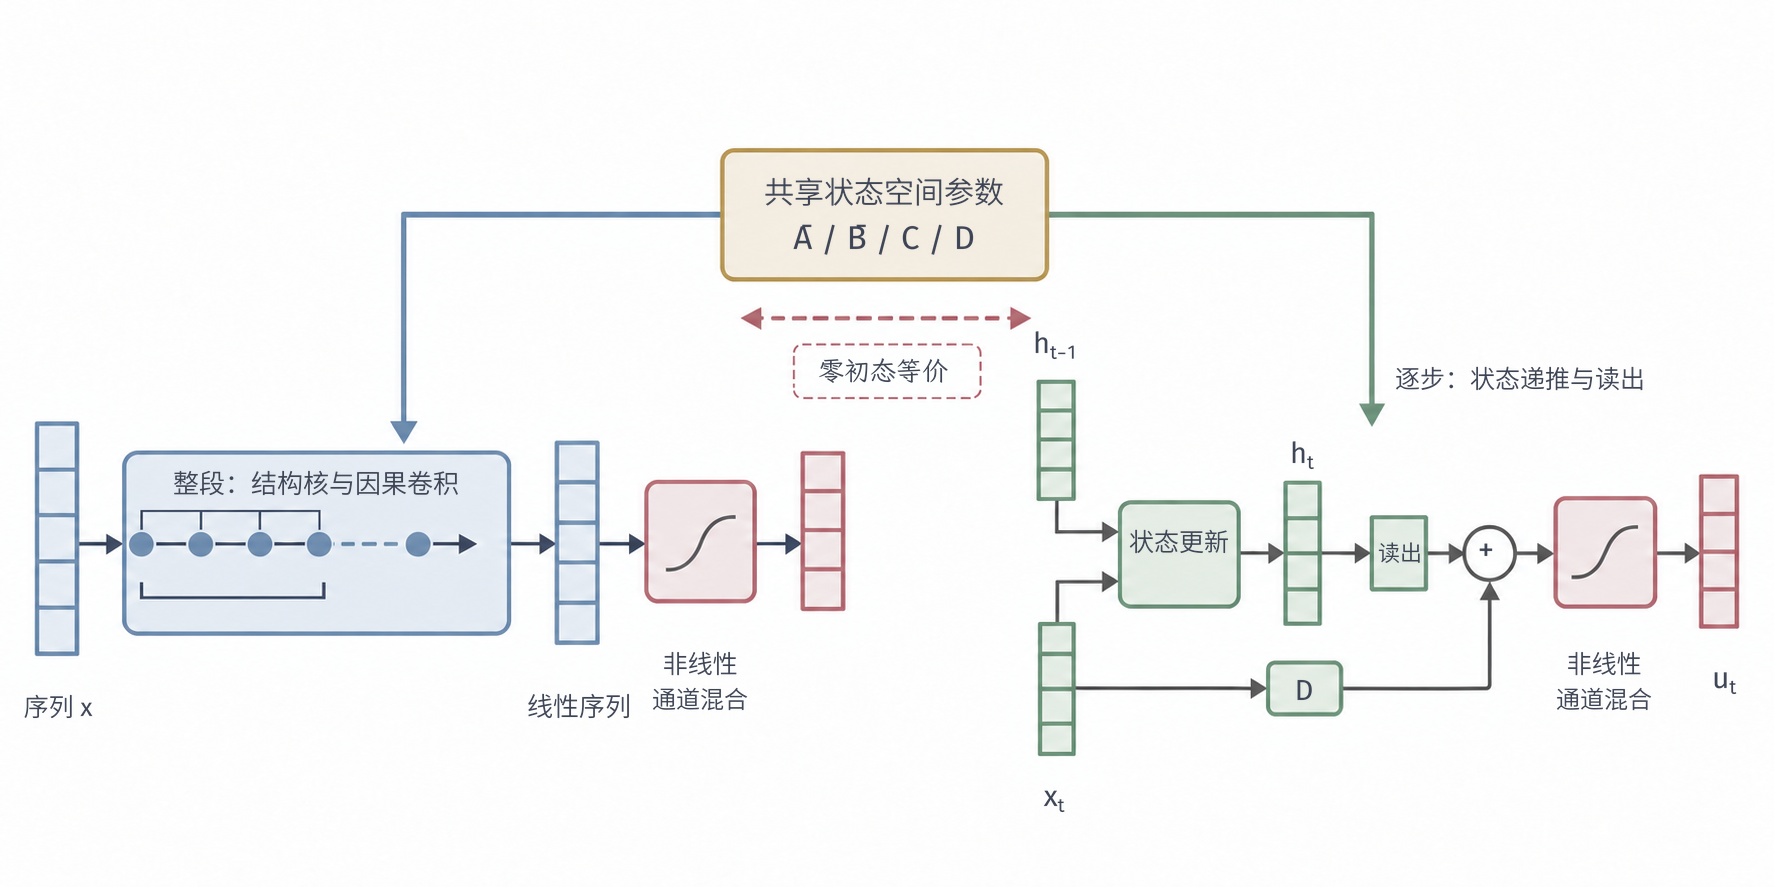
\includegraphics[width=150.199mm]{figures/05-neural-network-models/00-shared/generated/rnn-s4/figure.png}
  \caption{S4层的整段与逐步计算。两个路径共享同一组离散状态参数及后续通道映射，上方路径提供共享参数，跨路径虚线说明零初态下的等价关系。整段分支把直达映射$\bm D$并入零滞后卷积系数，$\widetilde{\bm K}_0=\bm K_0+\bm D$，其余滞后系数不变。零初态时，因果卷积与递推得到相同线性序列输出；非零初态需要补上对应初态响应。图中$\bm u$是层输出特征，任务预测还需相应读出。}
  \label{fig:rnn-s4}
\end{figure*}
\FloatBarrier

结构参数、输入输出映射、步长与通道映射由任务损失联合学习。卷积路径的反向计算对结构参数所生成的同一个核求导；预测切到递推时，需要使用与训练一致的离散化、因果约定和初始化。整个网络可以非线性，卷积等价只针对满足LTI条件的状态模块。

HiPPO-LegS的$1/\tau$更新与S4中的固定结构动态也应分清。S4借用结构矩阵和初始化思想，使网络可以学习有用的时间响应；当前模块的固定动态与LegS随历史区间扩展的更新有不同的时间含义。DPLR结构首先服务于高效计算，训练后的稳定性与长期响应还要检查参数取值。

\subsubsection{时间尺度与长期依赖}
\label{sec:rnn-s4-long-memory}

S4保存多久，与离散状态矩阵的模式有关。在可对角化情形下，$\bm K_k=\bm C\overline{\bm A}^k\overline{\bm B}$是多个指数模式的加权组合。某模式的特征值$\bar\lambda_j$满足$0<|\bar\lambda_j|<1$时，其幅度按$|\bar\lambda_j|^k$衰减，相应以步数计的时间尺度为
\begin{equation}
  \tau_{\mathrm{steps},j}=-\frac{1}{\log|\bar\lambda_j|}\text{。}
  \label{eq:rnn-s4-timescale}
\end{equation}
幅度经过这个步数约降到原来的$e^{-1}$。接近1的模式保留较久，较小的模式强调近期；复数模式还可表示振荡。不同时间尺度共同形成历史响应，输入映射决定往哪些模式写入，输出映射决定哪些模式参与预测。

对连续特征值$\lambda_j$，双线性离散化给出$\bar\lambda_j=(1+\Delta\lambda_j/2)/(1-\Delta\lambda_j/2)$。左半平面的特征值映入单位圆内，步长又改变离散时间尺度。特征值只描述模式，非正规矩阵的短期放大与数值条件仍需考虑；结构可高效计算，也不代表任意自由参数都稳定。

长期影响在输入输出层面写为$\partial\bm y_t/\partial\bm x_s=\bm K_{t-s}$，$s<t$；当前输入的导数还包含直接项$\bm D$。卷积路径直接计算这个历史响应，训练时不必按普通RNN的非线性单元逐步展开；但FFT与递推计算的是同一个映射，相关历史响应的导数也相同。若核在相关距离已经衰减，早期证据仍然弱；若读写映射没有利用慢模式，长时间尺度也不会自动转成任务所需的记忆。

S4因而同时改善状态的结构设计和整段计算。固定LTI模块对同一滞后使用同一响应，适合学习多尺度时间关系，却不能在单个模块中按每次输入的内容改写保留率。非线性堆叠扩展了网络表达，按内容选择状态的另一种做法则是下面的Mamba。

\subsection{Mamba}
\label{sec:rnn-mamba}

S4用固定的线性时不变动态换来了并行与长记忆，但“固定”也意味着它对所有输入一视同仁：无论当前内容是无关紧要的停用词还是需要牢记的关键事实，状态都按\emph{同一个}预设速率衰减和响应。可在真实语言中，需要记住的信息出现位置并不固定，理想的遗忘速度应\emph{随内容变化}——这正是LSTM门控解决过的问题，但LSTM又无法享受SSM的并行扫描。Mamba要把两者的优点合起来：\emph{让S4的部分系数由当前输入动态产生（选择性），同时保持状态更新对旧状态是仿射的，从而仍能用扫描并行}。\term{Mamba}让输入决定每一步的有效步长、写入和读出，改变哪些内容被写入、保留或读出。本节采用原始Mamba架构\scite{gu2023mamba}

\subsubsection{选择性状态更新}
\label{sec:rnn-mamba-selection}

为看清选择性，考察预处理后一个通道的标量输入$x_t$与$m$维状态。固定可学习的连续对角矩阵$\bm A$，由当前输入特征产生$\Delta_t>0$、$\bm B_t\in\mathbb R^m$和$\bm C_t\in\mathbb R^{1\times m}$，采用零阶保持时
\begin{equation}
  \begin{aligned}
    \overline{\bm A}_t&=\exp(\Delta_t\bm A),\\
    \overline{\bm B}_t&=\int_0^{\Delta_t}\exp(u\bm A)\bm B_t\,\mathrm du,\\
    \bm h^{(t)}&=\overline{\bm A}_t\bm h^{(t-1)}+\overline{\bm B}_t x_t,\\
    y_t&=\bm C_t\bm h^{(t)}+D x_t\text{。}
  \end{aligned}
  \label{eq:rnn-mamba-selection}
\end{equation}
$D$是通道的直接输入系数。输入相关不要求$\bm A$每步重新生成，选择性来自步长、写入和读出映射。多个通道各有状态，并由通道投影组合。

常用参数化令$A_{i,i}=-\exp(a_i)$、$\Delta_t=\operatorname{softplus}(d_t)$，其中$a_i$是参数，$d_t$由输入映射并加入偏置产生。这分别限制连续模式的衰减方向与步长的正值。$\bm B_t$决定输入写入哪些状态坐标，$\bm C_t$决定本步从哪些坐标形成输出。离散化是模型定义的一部分，复现时需核对写入项采用的具体规则。

取标量特例$A=-1$、$B_t=1$、$D=0$，更新成为
\begin{equation}
  h^{(t)}=e^{-\Delta_t}h^{(t-1)}+(1-e^{-\Delta_t})x_t\text{。}
  \label{eq:rnn-mamba-gate-special-case}
\end{equation}
小步长主要保留旧状态，大步长更多采用当前输入。这与控制门有明确联系，但完整模块具有多个状态坐标及输入相关的读写映射，其读写自由度由完整状态和各选择映射共同确定。

\subsubsection{完整模块的两条分支}
\label{sec:rnn-mamba-architecture}

选择性SSM只负责时间方向的状态计算。图~\ref{fig:rnn-mamba}把它放回完整模块：输入归一化与投影后分成两条支路，一条经过短因果卷积和SiLU，产生送入SSM的特征；另一条经过SiLU形成调制向量。SSM输出与调制向量逐坐标相乘，再经过输出投影和残差相加。

本例的归一化在每个样本、每个位置的特征坐标内计算，只根据当前位置的特征形成所需统计量，不把其他时间位置的值合入统计范围。整段训练时也逐位置应用同一规则，因此该步骤不会读取未来输入；下面的短卷积和选择性状态更新再按因果顺序处理时间依赖。
\begin{figure*}[htb]
  \centering
  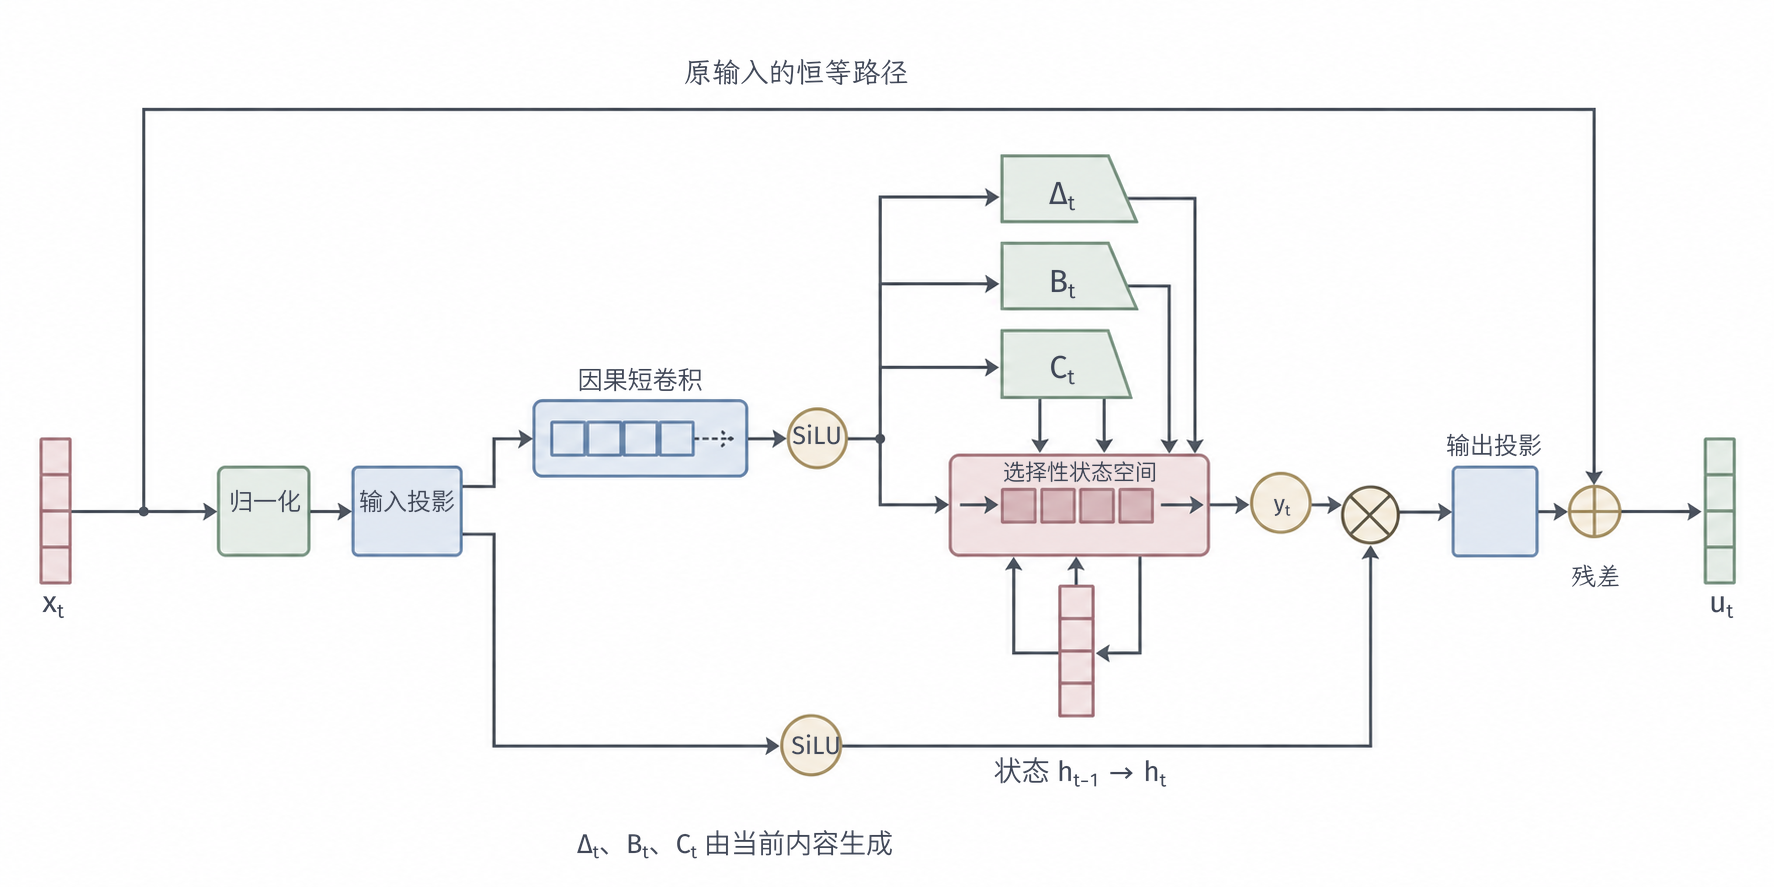
\includegraphics[width=150.199mm]{figures/05-neural-network-models/00-shared/generated/rnn-mamba/figure.png}
  \caption{原始Mamba模块的主要计算路径。选择参数分支说明选择性的来源：短卷积后的输入特征生成$\Delta_t,\bm B_t,\bm C_t$，并据此调节SSM更新；另一路特征调制SSM输出，上方直达线完成跨层残差。$\bm u_t$是模块输出，任务预测由后续网络读出。图中省略短卷积缓存、批次维和跨通道广播细节。}
  \label{fig:rnn-mamba}
\end{figure*}
\FloatBarrier

令归一化输入为$\widetilde{\bm x}_t\in\mathbb R^d$，内部通道数为$d_{\mathrm{in}}$，可将这两条支路写为
\begin{equation}
  \begin{aligned}
    \bm v_t&=\operatorname{SiLU}\!\left(\operatorname{CausalConv}
                (\bm W_{\mathrm v}\widetilde{\bm x})_t\right),\\
    \bm z_t&=\operatorname{SiLU}(\bm W_{\mathrm z}\widetilde{\bm x}_t),\\
    \bm y_t&=\operatorname{SelectiveSSM}(\bm v_{1:t}),\\
    \bm u_t&=\bm x_t+\bm W_{\mathrm{out}}(\bm y_t\odot\bm z_t)\text{。}
  \end{aligned}
  \label{eq:rnn-mamba-block}
\end{equation}
$\bm W_{\mathrm v},\bm W_{\mathrm z}\in\mathbb R^{d_{\mathrm{in}}\times d}$，$\bm W_{\mathrm{out}}\in\mathbb R^{d\times d_{\mathrm{in}}}$。各通道的选择系数由$\bm v_t$产生，$\bm y_t,\bm z_t$均为内部通道向量。SiLU调制支路缩放本步输出，其系数并未限制到$[0,1]$；时间记忆的保留率则来自SSM中的步长与状态参数。短卷积补充局部上下文，残差提供层方向的直达路径，各自作用不同。

\subsubsection{扫描、学习与计算代价}
\label{sec:rnn-mamba-scan}

输入相关系数使响应依赖具体输入和绝对位置，一般不能继续使用一个固定卷积核。不过，整段输入给定后，各步系数可先从输入计算；状态更新对旧状态仍是仿射的，对角结构又使组合便宜，所以能够使用式\eqref{eq:rnn-affine-composition}的扫描。若系数还依赖尚未算出的旧状态，就不能直接套用这种预先形成各步变换的方式，这也是它与一般LSTM／GRU计算组织的差别。

硬件感知的选择性扫描把离散化与状态更新放在适当存储层次中计算，避免在较慢存储中显式写出所有通道、所有位置的扩展状态；反向时可以重算中间量。扫描与重算改变计算顺序和存储策略，任务损失仍对同一递推求导。输入输出投影、短卷积、选择映射、状态参数与步长参数共同学习，选择哪些输入不是人工指定的必然结果。

设内部通道数为$d_{\mathrm{in}}$、每通道状态宽度为$m$，状态更新工作量为$O(Td_{\mathrm{in}}m)$，逐步持久状态为$O(d_{\mathrm{in}}m)$，还需短卷积和移位缓存。通道投影另有每步$O(dd_{\mathrm{in}})$成本。定长预测状态与高效整段扫描降低了计算负担，训练仍需优化器状态和相应反向信息，因此训练存储还随反向图、重算策略和优化器配置变化。

\subsubsection{有效时间与长期保留}
\label{sec:rnn-mamba-long-memory}

固定输入产生的系数，跨步状态扰动沿齐次路径传播为
\begin{equation}
  \frac{\partial\bm h^{(t)}}{\partial\bm h^{(s)}}
    =\exp\!\left(\bm A\sum_{u=s+1}^{t}\Delta_u\right)\text{，}
  \label{eq:rnn-mamba-memory-product}
\end{equation}
因为同一对角矩阵的指数可以相乘后合并。传播尺度由累计的内部步长决定：遇到无关输入时，若模型产生小$\Delta_u$，经过很多位置也可以只积累较少衰减；需要更新时再加大步长，并通过$\bm B_u$写入新内容。这将固定的逐步衰减变成内容相关的“有效经过时间”。

仍用式\eqref{eq:rnn-mamba-gate-special-case}作构造例子：从零状态读入$x_1=1$，取$\Delta_1=\log2$，得到$h^{(1)}=1/2$。其后100步输入为零且步长均为$0.001$，末状态为$(1/2)e^{-0.1}\approx0.452$。这个例子展示小步长如何弱化中间位置的遗忘；真实任务还要学到哪些位置应如此处理，且写入项的大小同时受$\bm B_t$和输入影响。

选择性更新把历史概括为定长状态。$\bm C_t$读取这些状态坐标，逐位置注意力则另存过去表示供本次查询评分；状态容量、输入干扰与有限精度仍限制可区分历史。系数对输入的导数、层间非线性和调制支路也进入完整梯度。选择机制提供了保留和覆盖的自由，扫描使这种机制便于计算，实际长期读取能力由保留规则、有限状态容量与任务学习共同决定。

% 完整作者列表较长，保留足够空间容纳本节开头的边注文献。
\Needspace{105mm}
\subsection{RWKV}
\label{sec:rnn-rwkv}

Mamba用选择性扫描获得了内容相关的记忆与并行性，RWKV则从另一个角度追求同样的目标：能否构造一个\emph{形式上完全是线性递推、只靠定长状态就能逐步生成}的模型，同时又像注意力那样让历史值的权重由“内容相似度”和“时间远近”共同决定？这样既保留RNN推理时状态恒定、显存不随序列变长的优点，又能在训练时把递推展开成可并行的加权求和。\term{接收门加权键值网络}（receptance weighted key value, RWKV）以时间混合和通道混合两种操作构成模块：历史值由内容权重与时间衰减共同累积成两个向量状态，再由一个接收门控制输出多少。本节采用2023年论文中的RWKV-4形式；后续版本的状态形状和更新可能不同\scite{peng2023rwkv}

\subsubsection{时间混合与加权状态}
\label{sec:rnn-rwkv-time-mixing}

设时间混合子模块的输入为$\bm{x}_t\in\mathbb{R}^{d}$，在完整层中它已由\term{层归一化}（layer normalization, LN）得到。这里LN只对同一位置的$d$个特征坐标计算均值与方差，标准化后再作可学习的逐坐标缩放和平移，各位置共享这些参数；具体公式见式\eqref{eq:transformer-layernorm}。它不跨样本或时间位置统计，因此归一化本身不会读取未来输入。时间混合先在当前与前一步输入之间逐坐标混合，再投影为键、值和接收向量：
\begin{equation}
  \bm{a}_t=\bm{W}_{\mathrm{a}}\!\left(
    \bm{\mu}_{\mathrm{a}}\odot\bm{x}_t
    +(\bm{1}-\bm{\mu}_{\mathrm{a}})\odot\bm{x}_{t-1}\right),
  \quad \mathrm{a}\in\{\mathrm{k},\mathrm{v},\mathrm{r}\}\text{。}
  \label{eq:rnn-rwkv-time-mixing}
\end{equation}
其中$\bm{\mu}_{\mathrm{a}}\in\mathbb{R}^{d}$是可学习混合系数，$\bm{W}_{\mathrm{a}}\in\mathbb{R}^{d\times d}$；$\bm{k}_t,\bm{v}_t,\bm{r}_t$分别取$\bm{a}_t$的对应结果。序列起始时的前一步输入需按约定初始化。

所有指数、除法和乘积按坐标进行。令非负衰减参数为$\bm{w}\in\mathbb{R}^{d}$，当前项偏置为$\bm{u}\in\mathbb{R}^{d}$，历史分子和分母状态初值为零，则
\begin{equation}
  \begin{aligned}
    \bm{v}_{\mathrm{agg}}^{(t)}&=
      \frac{\bm{a}^{(t-1)}+e^{\bm{u}+\bm{k}_t}\odot\bm{v}_t}
           {\bm{b}^{(t-1)}+e^{\bm{u}+\bm{k}_t}},\\
    \bm{a}^{(t)}&=e^{-\bm{w}}\odot\bm{a}^{(t-1)}
                    +e^{\bm{k}_t}\odot\bm{v}_t,\\
    \bm{b}^{(t)}&=e^{-\bm{w}}\odot\bm{b}^{(t-1)}+e^{\bm{k}_t},\\
    \bm{o}_t&=\bm{W}_{\mathrm{o}}\!\left(
      \operatorname{sigmoid}(\bm{r}_t)\odot\bm{v}_{\mathrm{agg}}^{(t)}\right)\text{。}
  \end{aligned}
  \label{eq:rnn-rwkv-recurrence}
\end{equation}
输出在历史状态更新前读取旧累积量，并为当前项使用$\bm{u}$；之后写入状态的当前项不包含该偏置。展开分子可见，第$i<t$个位置的权重为$\exp(-(t-1-i)\bm{w}+\bm{k}_i)$。它取决于该位置的键和时间距离，接收门再决定每个通道输出多少，没有对每个历史位置重新计算查询—键点积。

可以用两个位置的计算区分“当前怎样读出”和“历史怎样保存”。只看一个通道，取$w=\log2$、$u=\log3$，两个位置的键均为零，值依次为$v_1=2$、$v_2=0$。第一步没有历史，聚合值为2，写入后$a^{(1)}=2,b^{(1)}=1$。第二步读出时，旧值的权重为1，当前值的权重为3，因此聚合值为$(2+3\times0)/(1+3)=1/2$。随后保存历史时，旧贡献衰减一半，当前贡献按权重1写入，得到$a^{(2)}=1,b^{(2)}=3/2$。这两个新状态留给下一步使用，不能用它们的比值替代本步的聚合值；本步还要经过接收门和输出投影，才得到$\bm o_t$。

状态递推证明了过去的加权和可以由两个向量维护，不必逐步保存全部键值。直接指数形式容易上溢，实际实现还维护尺度或最大值，使用重缩放保持与上述比值等价。分母在非空步由正指数项保证为正；数值实现需要这种重缩放来控制指数范围。

\subsubsection{通道混合与完整残差层}
\label{sec:rnn-rwkv-architecture}

时间混合负责历史累积，\term{通道混合}（channel mixing）则在当前表示中组合不同特征。它也用当前与前一步输入作混合，但不重复WKV的历史加权和。令相应子模块输入仍记为$\bm x_t\in\mathbb R^d$，可写为
\begin{equation}
  \begin{aligned}
    \bm k'_t&=\bm W'_{\mathrm k}\left(\bm\mu'_{\mathrm k}\odot\bm x_t
          +(\bm1-\bm\mu'_{\mathrm k})\odot\bm x_{t-1}\right),\\
    \bm r'_t&=\bm W'_{\mathrm r}\left(\bm\mu'_{\mathrm r}\odot\bm x_t
          +(\bm1-\bm\mu'_{\mathrm r})\odot\bm x_{t-1}\right),\\
    \bm o'_t&=\operatorname{sigmoid}(\bm r'_t)\odot
         \bm W'_{\mathrm v}\left(\operatorname{ReLU}(\bm k'_t)
                              \odot\operatorname{ReLU}(\bm k'_t)\right)\text{。}
  \end{aligned}
  \label{eq:rnn-rwkv-channel-mixing}
\end{equation}
若内部宽度为$d_{\mathrm{ff}}$，则$\bm W'_{\mathrm k}\in\mathbb R^{d_{\mathrm{ff}}\times d}$、$\bm W'_{\mathrm v}\in\mathbb R^{d\times d_{\mathrm{ff}}}$，$\bm W'_{\mathrm r}\in\mathbb R^{d\times d}$。平方ReLU提供非线性通道变换，接收门调节其输出。混合系数是可学习参数，若没有额外约束，不保证它们一直处于$[0,1]$。

图~\ref{fig:rnn-rwkv}先给出完整残差层，再用虚线把时间混合子模块A与其内部计算对应起来。下方的输出$\bm o_t$就是上方A送入第一个残差加法的量；通道混合B随后处理更新的表示。在完整层公式中，$\bm x_t$改指归一化之前的层输入，$\bm s_t$表示第一次残差相加后的中间量，区别于WKV中的值向量$\bm v_t$。典型的归一化与残差关系为
\begin{equation}
  \begin{aligned}
    \bm s_t&=\bm x_t+\operatorname{TimeMix}
                    (\operatorname{LN}_1(\bm x_t)),\\
    \bm u_t&=\bm s_t+\operatorname{ChannelMix}
                    (\operatorname{LN}_2(\bm s_t))\text{。}
  \end{aligned}
  \label{eq:rnn-rwkv-residual-layer}
\end{equation}
LN是逐位置层归一化，状态更新在各子模块内部进行。时间混合与通道混合分别缓存各自归一化后进入子模块的前一步输入；两份缓存对应不同阶段的表示。完整生成网络在嵌入之后堆叠这些层，再用归一化和词表投影形成下一词元的概率。
\begin{figure*}[t]
  \centering
  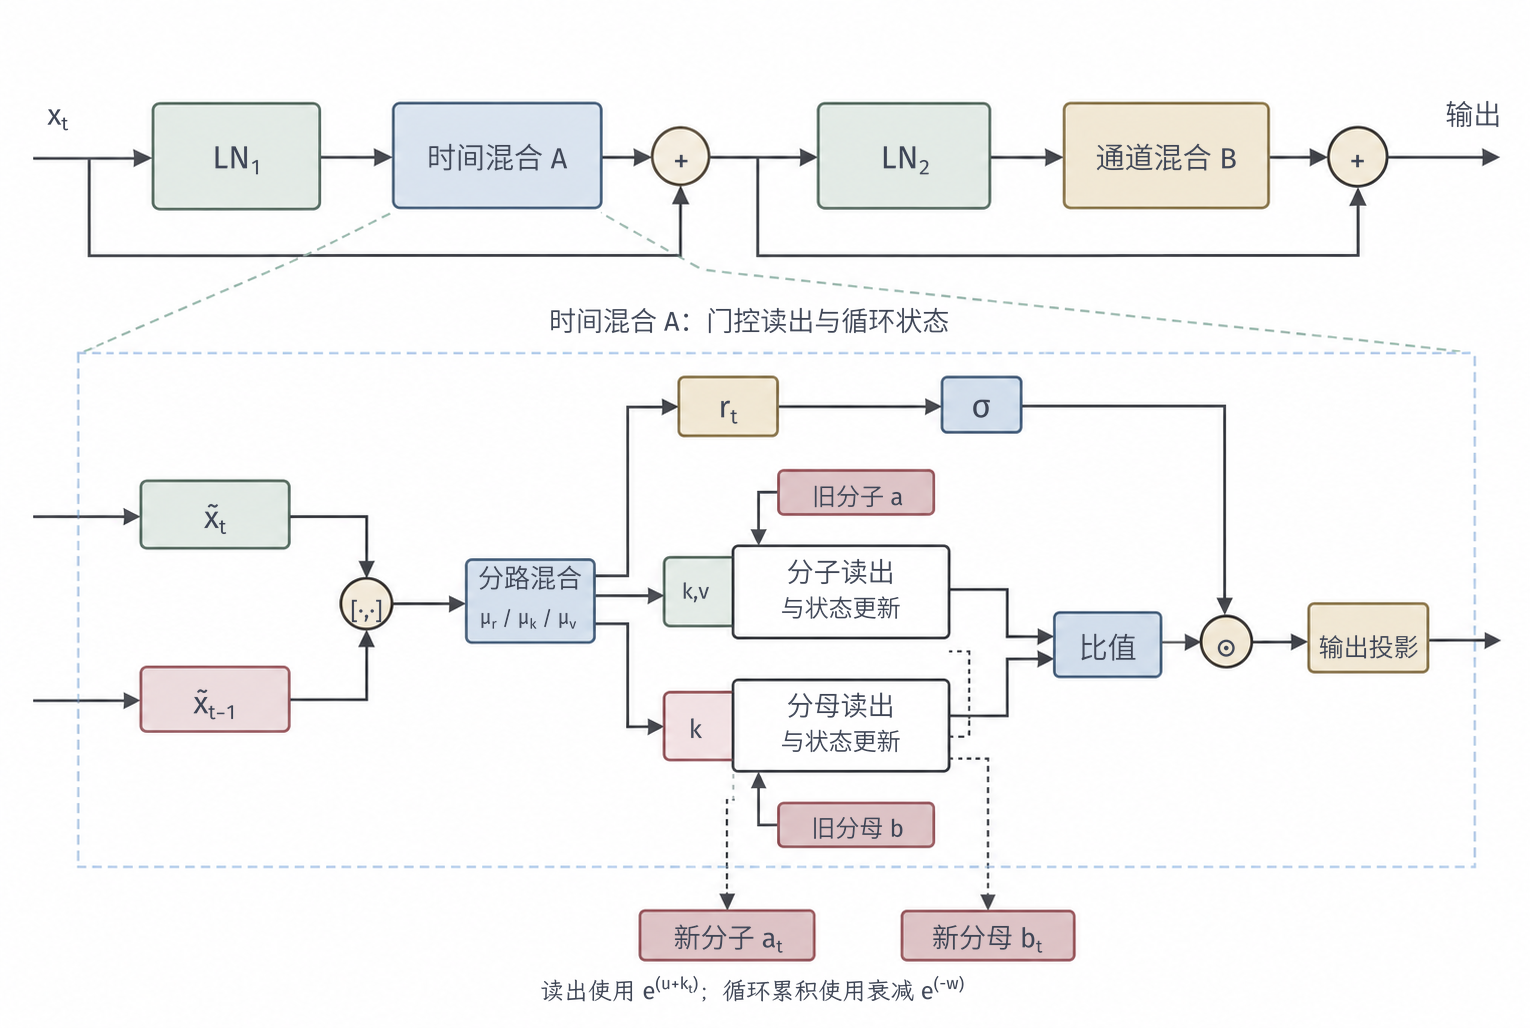
\includegraphics[width=129.540mm]{figures/05-neural-network-models/00-shared/generated/rnn-rwkv/figure.png}
  \caption{RWKV-4的完整残差层与时间混合子模块。上方在A、B之前分别归一化，并在各子模块之后作残差相加，第一次相加得到$\bm s_t$。下方只展开A，无箭头虚线表示对应关系；$\widetilde{\bm x}_t=\operatorname{LN}_1(\bm x_t)$是归一化后的特征。左下圆圈将当前与前一步的归一化输入打包为有序对，不把它们相加；分路混合分别采用$\bm\mu_r$、$\bm\mu_k$、$\bm\mu_v$，再形成各自的投影。下方展开分子、分母状态与读出之间的关系：循环更新使用$e^{-\bm w}$衰减，读出中另含当前键的$e^{\bm u+\bm k_t}$权重；精确递推见正文公式。图中省略稳定化重缩放、移位缓存的保存箭头及B的内部计算。}
  \label{fig:rnn-rwkv}
\end{figure*}
\FloatBarrier

沿图中的路径处理一个新词元时，先由A把历史累积与当前特征结合，产生对层输入的修正；第一次残差相加后，B再组合这一表示中的特征，产生第二次修正。因此，A的输出并不是下一词元的概率，完整层的输出也还需要后续层与词表读出。图中的两个子模块依次工作，却各自保留前一步的输入：A缓存的是上一位置进入时间混合的归一化表示，B缓存的是上一位置经过第一次残差相加后再归一化的表示。若把两份缓存混用，就改变了各自混合的对象。

逐词生成时，每一层都延续自己的累积状态和两份输入缓存。新词元从底层向上经过各层后，这些状态更新到同一个时间步，下一个词元便从此继续；不必重新处理已经读过的整个前缀。开始一条独立序列时，则需要重新初始化这些状态，避免上一条序列的信息进入当前预测。生成过程中，各层状态和门的取值随输入变化，用于计算它们的模型参数保持不变。

训练时，各位置的稠密投影可以批量计算，WKV核心仍处理有序累积；可使用顺序扫描，满足组合条件时也可采用并行前缀计算。投影、混合系数、衰减及门由任务损失共同更新。逐步预测则只延续累积、移位与数值尺度状态。按$d$个通道计，累积核心整段为$O(Td)$、持久状态为$O(d)$，稠密投影另有每步$O(d^2)$或$O(dd_{\mathrm{ff}})$成本；层数、词表与训练反向信息需另外计算。

\subsubsection{归一化权重与长期依赖}
\label{sec:rnn-rwkv-long-memory}

RWKV没有在累积状态上反复施加普通RNN的稠密非线性变换，旧贡献沿各通道按$e^{-w_i}$保留。较小的$w_i$提供较长时间尺度，较大的值强调近期；内容键再改变各位置写入的权重。对固定键与衰减，某个历史值坐标对当前聚合的直接系数是归一化权重：
\begin{equation}
  \frac{\partial v_{\mathrm{agg},j}^{(t)}}{\partial v_{i,j}}
     =\frac{\exp(-(t-1-i)w_j+k_{i,j})}
       {b_j^{(t-1)}+\exp(u_j+k_{t,j})},\qquad i<t\text{。}
  \label{eq:rnn-rwkv-value-gradient}
\end{equation}
它取决于内容与时间距离，不是一个任意非线性状态Jacobian矩阵的连乘。完整任务梯度还包含接收门、输出投影以及键变化的路径，并受归一化权重的尺度影响。

归一化约束了加权聚合的范围，却不取消遗忘。先单看历史贡献的未归一化权重。若$w_j>0$，早期权重仍会随距离指数减弱；实际读出的归一化系数还要除以当前分母，不能仅由这个衰减因子确定。即使$w_j=0$、所有键相同且当前偏置为零，单个位置的权重也会随位置数按$1/t$稀释。较大内容权重可以让某些位置更突出，但并未建立对每个历史位置重新执行查询的机制。

压缩还会合并不同历史。例如只看一个$w=0$、全部键为零的累积核心，值序列$(1,0,0)$与$(0,1,0)$都产生分子1、分母3。它们的位置不同，两个累积量却相同；只依据这组状态无法区分证据曾出现在哪一步。多通道、移位和深层非线性增加了可用表示，但仍需依据具体任务检查压缩后的可区分性。

RWKV因此用内容加权、可学习衰减和接收门组织可延续的历史，使训练投影便于批量计算、预测状态保持定长。它缓解了一部分普通非线性循环路径的困难，保留范围与检索能力仍由时间尺度、写入权重、层间计算和任务监督共同决定。

表~\ref{tab:rnn-state-models}统一比较上述状态模块。HiPPO是一套状态构造原则，S4、Mamba和RWKV是利用特定结构组织序列计算的网络设计，比较时分别记录状态构造原则、实际网络更新与计算组织，便于看出它们的组合关系。

\begin{table*}[htb]
  \small
  \begin{tabularx}{\linewidth}{@{}p{19mm}XXX@{}}
    \toprule
    模型或原则 & 历史表示与选择 & 整段计算 & 逐步持久状态 \\
    \midrule
    普通RNN & 非线性隐藏状态；全部坐标经共同更新 & 时间递推与BPTT & 单层$m$维状态 \\
    LSTM／GRU & 门调节保留和写入；LSTM另有记忆状态 & 通常逐步递推 & 等宽LSTM为$2m$，GRU为$m$ \\
    HiPPO & 基函数系数；测度与阶数决定近似范围 & 取决于所选更新与离散化 & $m$个投影系数 \\
    S4 & 结构化线性状态；固定时间响应 & LTI模块可用结构核与FFT卷积 & 每通道$m$维状态 \\
    Mamba & 输入相关步长、写入与读出 & 选择性仿射扫描 & $d$通道共$dm$维状态，另有短卷积缓存 \\
    RWKV-4 & 内容加权累积、时间衰减与接收门 & 批量投影和加权扫描等 & 两组累积向量及移位、数值尺度缓存 \\
    \bottomrule
  \end{tabularx}
  \caption{历史压缩与计算方式的比较。这里$m$表示状态宽度，$d$表示通道数，均按单层比较；持久状态只计流式预测中需延续的信息，不含参数、输出缓存和反向传播激活。稠密投影、层数与数值实现会改变完整网络的计算和存储。}
  \label{tab:rnn-state-models}
\end{table*}
\FloatBarrier

定长状态的代价不随已读长度线性增加，但相同宽度并不意味着相同的信息容量。循环注意力保存各位置编码状态，付出随输入长度增长的存储与读取；压缩状态把这一要求转为历史如何概括。两类模型的取舍应结合任务所需的精确位置访问、预测延迟和输入范围判断。

\FloatBarrier
\section{循环神经网络的扩展}
\label{sec:rnn-extensions}

此前的模型都沿一条单一的时间链组织状态：每个位置只看它前面的那一个位置。实际任务会在两个方向上突破这条链。其一是\emph{拓扑}：信息也许需要同时看到后文（双向）、沿图像的多个空间方向流动（多维），或按语法树那样的层次结构组合（树递归）——拓扑决定了一个状态在计算时能看到哪些对象。其二是\emph{深度}：同一位置的表示也可以像前馈网络那样纵向堆叠多层，让较低层形成局部特征、较高层在同一时刻做更抽象的组合——深度决定同一位置经历多少次表示变换。

\subsection{支持不同的拓扑结构}
\label{sec:rnn-topologies}

\subsubsection{双向循环与信息可见范围}
\label{sec:rnn-bidirectional}

许多离线序列任务（如给已经写好的句子逐词标注词性）在做某个位置的判断时，\emph{后文也是合法可见的}。而单向状态$\bm h^{(t)}$按定义只读取$\bm x_1,\ldots,\bm x_t$，天然看不到右侧。\term{双向循环网络}（bidirectional RNN）的做法很直接：用两套参数独立的循环网络，一套从左向右、一套从右向左读取同一序列，再在每个位置把两个方向的状态拼成该位置的表示：
\begin{equation}
  \begin{aligned}
    \overrightarrow{\bm{h}}^{(t)}&=F_{\rightarrow}\!\left(
       \overrightarrow{\bm{h}}^{(t-1)},\bm{x}_t\right),\\
    \overleftarrow{\bm{h}}^{(t)}&=F_{\leftarrow}\!\left(
       \overleftarrow{\bm{h}}^{(t+1)},\bm{x}_t\right),\\
    \bm{h}_t&=[\overrightarrow{\bm{h}}^{(t)};
                 \overleftarrow{\bm{h}}^{(t)}]\text{。}
  \end{aligned}
  \label{eq:rnn-bidirectional}
\end{equation}
两向通常使用不同参数，分别从序列两端的初态开始。反向上标$(t)$仍对齐输入位置，计算次序却是$T,T-1,\ldots,1$。两条链在同一步不必互相反馈，组合后的表示交给读出或下一层。

双向表示能使用后文，前提是后文在预测时已经可见。实时下一步预测若把尚未到达的观测送入反向链，就泄漏了未来信息；整段编码器用于转换任务则可以合法读取完整源序列。预测时已知哪些输入，决定了当前状态可采用哪一条信息路径。

\subsubsection{多维与多方向循环}
\label{sec:rnn-multidimensional}

规则网格中的当前位置可以依赖多个已计算的邻居。\term{多维循环网络}（multi-dimensional RNN）沿网格上的有向顺序组合这些前驱状态。例如二维网格的一个方向可采用
\begin{equation}
  \bm{h}_{i,j}=\tanh\!\left(
     \bm{U}\bm{x}_{i,j}+\bm{W}_1\bm{h}_{i-1,j}
      +\bm{W}_2\bm{h}_{i,j-1}+\bm{b}\right)\text{。}
  \label{eq:rnn-multidimensional}
\end{equation}
网格边界上的缺失前驱按约定初始化。该方向只读取上方和左方已形成的表示；按$i+j$分组时，同一对角线的节点可并行，而后续对角线依赖此前结果。再以其他角落为起点建立多个方向，就能组合不同象限的上下文\scite{graves2007mdrnn}

这里的多方向不是对同一条序列多跑几次，而是改变前驱关系。梯度沿多个前驱分支回传，对共享参数累积所有位置的贡献。直接把多路记忆相加还会增加状态幅度，门控、归一化和组合规则需随前驱数量设计；稳定性也要按新增前驱和完整组合规则分析。

\subsubsection{树递归与Tree-LSTM}
\label{sec:rnn-tree}

当输入本身带有语法树或层次结构时，强行按词的线性先后顺序组合未必合理：一个词最该先与谁结合，由句法关系而非相邻位置决定。\term{树递归网络}（recursive neural network）改为按树的父子依赖自底向上组合状态：先算出所有子节点的表示，再在父节点把它们合成更大子结构的表示，直到根节点得到整句表示。名称中的recursive描述的是\emph{结构上的递归}，与沿时间重复更新的recurrent不是一回事；本章把二者都放在“隐状态按某种依赖递推”的统一框架下比较。

二叉树可以把左右子状态拼接后变换；子节点数不固定时，可以先求和聚合。\term{树结构长短期记忆}（Tree-LSTM）为每个子节点设置遗忘门，以不同权重组合其记忆。以Child-Sum版本为例，令$C(j)$是节点$j$的子节点索引集合，$\bm{x}_j$是本节点输入，$\bm{h}_j,\bm{c}_j$分别为隐藏和记忆状态，计算
\begin{equation}
  \begin{aligned}
    \overline{\bm{h}}_j&=\sum_{k\in C(j)}\bm{h}_k,\\
    \bm{i}_j&=\operatorname{sigmoid}\!\left(
       \bm{U}_{\mathrm{i}}\bm{x}_j+\bm{W}_{\mathrm{i}}\overline{\bm{h}}_j
       +\bm{b}_{\mathrm{i}}\right),\\
    \bm{o}_j&=\operatorname{sigmoid}\!\left(
       \bm{U}_{\mathrm{o}}\bm{x}_j+\bm{W}_{\mathrm{o}}\overline{\bm{h}}_j
       +\bm{b}_{\mathrm{o}}\right),\\
    \widetilde{\bm{c}}_j&=\tanh\!\left(
       \bm{U}_{\mathrm{c}}\bm{x}_j+\bm{W}_{\mathrm{c}}\overline{\bm{h}}_j
       +\bm{b}_{\mathrm{c}}\right),\\
    \bm{f}_{j,k}&=\operatorname{sigmoid}\!\left(
       \bm{U}_{\mathrm{f}}\bm{x}_j+\bm{W}_{\mathrm{f}}\bm{h}_k
       +\bm{b}_{\mathrm{f}}\right),\qquad k\in C(j),\\
    \bm{c}_j&=\bm{i}_j\odot\widetilde{\bm{c}}_j
        +\sum_{k\in C(j)}\bm{f}_{j,k}\odot\bm{c}_k,\\
    \bm{h}_j&=\bm{o}_j\odot\tanh(\bm{c}_j)\text{。}
  \end{aligned}
  \label{eq:rnn-tree-lstm}
\end{equation}
叶节点的空和为零，参数形状与等宽链式LSTM相同。求和对孩子的重编号不变，但会弱化孩子次序；若左右位置具有不同语义，采用带位置参数的有序树版本更合适。Tree-LSTM的代表工作分别讨论了这两类结构\scite{tai2015}

图~\ref{fig:rnn-topologies}将依赖范围与计算顺序并列展示。树上的反向传播从父节点回到各孩子，多个损失的贡献在同一节点汇合；共享组合参数的梯度再对所有节点累积。两个叶子经树组合到共同祖先的路径可以短于按词序遍历的路径，但这种优势依赖给定树是否符合任务，还增加了结构取得与处理的要求。

\begin{figure*}[t]
  \centering
  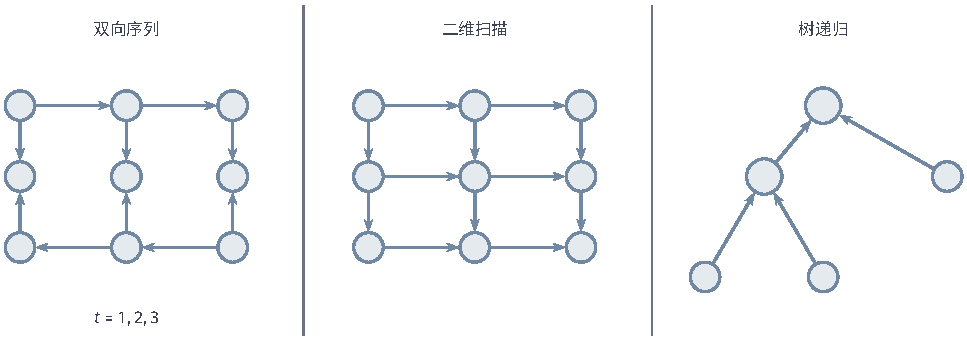
\includegraphics[width=163.791mm]{figures/05-neural-network-models/00-shared/tikz/rnn-topologies/figure.pdf}
  \caption{状态依赖拓扑。左图在同一输入位置组合正向与反向状态；中图由上方、左方前驱形成二维状态，箭头给出一个扫描方向；右图由叶节点向父节点组合子结构。圆节点表示各位置或子结构的状态，箭头表示状态依赖的方向。不同方向、位置或孩子组合是否共享参数，需要由具体模型说明。}
  \label{fig:rnn-topologies}
\end{figure*}
\FloatBarrier

例如，沿中图的箭头计算网格位置$(2,2)$时，直接使用的是$(1,2)$和$(2,1)$的状态。它们已经带来左上区域的信息，却尚未包含右侧$(2,3)$或下方$(3,2)$的输入。若任务需要这些区域的证据，就要增加从其他角落出发的方向，并在同一位置组合各方向的结果。左图的双向链采用同样的思路，让当前位置分别取得前文与后文的表示。

右图则改变了组合单位：两个叶子先在共同父节点形成局部子结构的表示，再与另一支的表示组合到根节点。这样，词语间的信息先后经过哪些状态，由给定树决定。选择拓扑时，首先要明确一次预测允许使用哪些输入，以及哪些输入应先组合；随后才能确定箭头、计算顺序和状态的含义。

\subsection{支持更深的网络}
\label{sec:rnn-depth}

时间展开的深度由序列长度决定，同一位置的表示变换深度则由层数决定。增加层数既可以让任务学习更多表示变换，也可以仅堆叠固定动态、提供更多历史特征。二者共享层次结构，却训练不同参数。

\subsubsection{堆叠循环网络：学习各层表示与时间动态}
\label{sec:rnn-stacked-networks}

\term{堆叠循环网络}（stacked RNN）让上层读取下层在相同位置的状态，同时维护自己的历史。设层数为$L$，$\bm h_0^{(t)}=\bm x_t$，则
\begin{equation}
  \bm h_{\ell}^{(t)}=F_{\ell}\!\left(\bm h_{\ell}^{(t-1)},
       \bm h_{\ell-1}^{(t)}\right),\qquad\ell=1,\ldots,L\text{。}
  \label{eq:rnn-stacked}
\end{equation}
上标是时间步，下标$\ell$是层索引。同一层跨步共享参数，不同层通常各用一组参数。单元可选普通RNN、LSTM或GRU；使用LSTM时，各层还维护自己的记忆状态$\bm c_\ell^{(t)}$。

第$t$步先计算底层，再把底层当前表示送到第二层，依次形成顶层表示。因而第二层同时读取“这一位置的底层特征”与“第二层此前形成的历史”。单向堆叠仍只使用当前及此前输入。

图~\ref{fig:rnn-stacked-network}展示三层网络的时间展开。水平箭头传递同层历史，垂直箭头传递同一时刻的层间表示。
\begin{figure}[htbp]
\centering
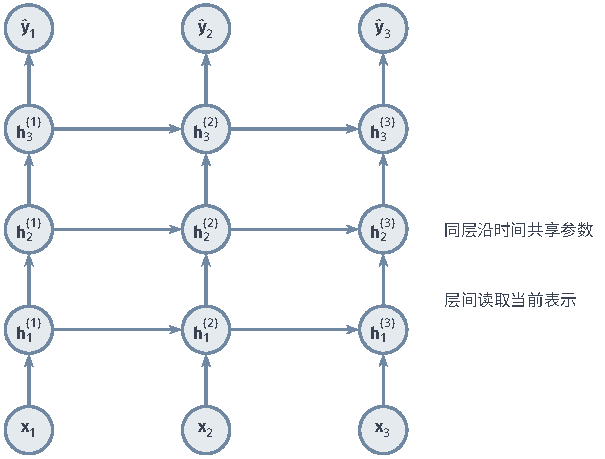
\includegraphics[width=102.369mm]{figures/05-neural-network-models/00-shared/tikz/rnn-stacked-network/figure.pdf}
\caption{三层堆叠循环网络。每层具有自己的循环参数并沿时间共享；上层读取下层当前状态与自身上一时刻状态，输出由顶层状态形成。图省略初态和层内门控。}
\label{fig:rnn-stacked-network}
\end{figure}
\FloatBarrier


以图中的第二个时间步为例，此时已保存三层在第一步的状态。输入$\bm x_2$先与$\bm h_1^{(1)}$形成$\bm h_1^{(2)}$，再由$\bm h_1^{(2)}$与$\bm h_2^{(1)}$形成$\bm h_2^{(2)}$，最后得到第三层的$\bm h_3^{(2)}$。这一次从底层到顶层的计算就完成了第二步；此前的输入$\bm x_1$通过各层保存的状态参与计算，无需重新输入。若单元采用LSTM，则每层还要同时更新并保存自己的$\bm c_\ell^{(2)}$。流式预测因此需要保存所有层的状态，单独保存顶层状态不足以继续下一步递推。

任务损失通常从顶层读出，也可以拼接或加权读取多个层。训练时梯度既沿时间回传，也沿层间依赖回传，各层循环与输入映射都接受任务监督。下层可以形成较局部的表示，上层再组合这些表示，但各层的时间尺度由实际动态和输入驱动决定，可以通过状态响应或任务行为检验。

若第$\ell$层宽度为$m_\ell$、$m_0=d$，普通稠密单元的整段计算量级为
\begin{equation}
  O\!\left(T\sum_{\ell=1}^{L}m_\ell(m_{\ell-1}+m_\ell)\right)\text{，}
  \label{eq:rnn-stacked-cost}
\end{equation}
门控单元还增加相应常数。完整反向计算需保存或重算各层各步的激活。层宽、读出范围与训练存储因此都影响深度选择。

\subsubsection{深度储备池计算：堆叠固定动态、学习统一读出}
\label{sec:rnn-deep-reservoir}

\term{深度储备池计算}（deep reservoir computing）把多个通常固定的储备池按层连接，利用层层动态形成历史特征，再训练任务读出。深度ESN是代表形式，第一层读取外部输入，上层读取下层当前状态\scite{gallicchio2018deepesn}

对泄漏积分单元，可写为
\begin{equation}
  \begin{aligned}
    \bm h_\ell^{(t)}&=(1-\alpha_\ell)\bm h_\ell^{(t-1)}
      +\alpha_\ell\tanh\!\left(\bm W_\ell\bm h_\ell^{(t-1)}
               +\bm U_\ell\bm h_{\ell-1}^{(t)}+\bm b_\ell\right),\\
    \widehat{\bm y}_t&=g\!\left(\bm V
       [1;\bm x_t;\bm h_1^{(t)};\ldots;\bm h_L^{(t)}]\right)\text{。}
  \end{aligned}
  \label{eq:rnn-deep-esn}
\end{equation}
$0<\alpha_\ell\leq1$是各层泄漏率，$\bm W_\ell,\bm U_\ell,\bm b_\ell$按构造固定，$\bm V$是可训练读出矩阵；也可以只读部分层。训练先逐步收集拼接特征，再拟合读出，平方损失时仍是一组扩展特征上的岭回归，不需要为固定循环参数执行任务梯度更新。

层叠改变输入经过的动态过滤。在线性标量简化且循环矩阵为零时，$h^{(t)}=(1-\alpha)h^{(t-1)}+\alpha u_t$，记忆按$(1-\alpha)^k$衰减，对$0<\alpha<1$的时间尺度为$-1/\log(1-\alpha)$。这说明不同泄漏率可以提供不同更新速度；真实储备池还包含反馈矩阵、输入驱动与非线性，整个模型的时间响应由这些因素共同形成。

各层也要检查回声状态性质。设相同输入下的两条轨迹距离为$\delta_\ell^{(t)}$，Tanh的Lipschitz性质给出
\begin{equation}
  \delta_\ell^{(t)}\leq r_\ell\delta_\ell^{(t-1)}
       +\alpha_\ell\lVert\bm U_\ell\rVert_2\delta_{\ell-1}^{(t)},
  \quad r_\ell=1-\alpha_\ell+\alpha_\ell\lVert\bm W_\ell\rVert_2\text{。}
  \label{eq:rnn-deep-esn-contraction}
\end{equation}
外部输入相同时$\delta_0^{(t)}=0$。

为看清下层差异怎样影响上层，令$\kappa_\ell=\alpha_\ell\lVert\bm U_\ell\rVert_2$，把式\eqref{eq:rnn-deep-esn-contraction}沿时间反复代入，得到
\[
 \delta_\ell^{(t)}
 \leq r_\ell^t\delta_\ell^{(0)}
   +\kappa_\ell\sum_{s=1}^{t}r_\ell^{t-s}\delta_{\ell-1}^{(s)}\text{。}
\]
右侧第一项只传播本层的初始差异，第二项累积下层在各步传来的差异。第一层接收的外部输入差始终为零，所以当$r_1<1$时，$\delta_1^{(t)}\leq r_1^t\delta_1^{(0)}\to0$。第二层及以上仍可能在每一步收到非零的下层差异，需要控制整个加权和。

设已经知道$\delta_{\ell-1}^{(s)}\to0$，且$0\leq r_\ell<1$。对任意$\varepsilon_0>0$，可以固定一个步数$M$，使$s>M$时$\delta_{\ell-1}^{(s)}\leq\varepsilon_0$。在$t>M$时，将驱动和拆成早期与晚期两部分：
\[
 \begin{aligned}
 \sum_{s=1}^{t}r_\ell^{t-s}\delta_{\ell-1}^{(s)}
 &=\sum_{s=1}^{M}r_\ell^{t-s}\delta_{\ell-1}^{(s)}\\
 &\quad+\sum_{s=M+1}^{t}r_\ell^{t-s}\delta_{\ell-1}^{(s)}\text{。}
 \end{aligned}
\]
早期部分只有固定的有限项，每项都随$t\to\infty$趋于零；晚期部分满足
\[
 \sum_{s=M+1}^{t}r_\ell^{t-s}\delta_{\ell-1}^{(s)}
 \leq\varepsilon_0\sum_{j=0}^{t-M-1}r_\ell^j
 \leq\frac{\varepsilon_0}{1-r_\ell}\text{。}
\]
乘上有界的$\kappa_\ell$后，晚期部分仍可随$\varepsilon_0$任意变小。本层初态项和早期部分又都趋于零，因而$\delta_\ell^{(t)}\to0$。从第一层开始，对有限个层依次使用这一步，就得到整个层叠的初态遗忘；这里使用的是下层差异趋于零，并没有假定上层的驱动在每一步都为零。

有限层数、各$r_\ell<1$且层间映射有界时，下层初态差异逐渐消失，上层受其驱动的差异也能衰减。这是充分条件；上述推导把各层收缩与层间有界映射共同计入，整个层叠的初态遗忘由这一组合条件支持。

与可训练堆叠RNN相比，深度储备池减少了循环动态的优化范围，多个层的特征可供同一读出选择；代价是固定状态变换不能按任务梯度重新安排记忆。层数、宽度、连接尺度和泄漏率通常由验证过程选择，测试数据不能参与这种选择。更多固定层可能增加有用时间特征，也可能增加冗余或压缩损失，需要与浅层储备池在相近预算下比较。

\subsubsection{跨层连接与分层读出}
\label{sec:rnn-depth-connections}

可训练网络与固定储备池都可以改变层间连接。维度相同时，跨层残差可写为$\bm u_\ell^{(t)}=\bm h_{\ell-1}^{(t)}+G_\ell^{(t)}$，其中$G_\ell^{(t)}$是这一层产生的变换结果；维度不同时先投影直达分支。残差为层方向提供较直接的梯度路径，通常没有缩短同一层的时间路径。

分层读出把不同层的状态送到任务头，使监督或读出可以直接使用多个层次的特征；它扩大了读出输入与参数规模。跨时间跳跃、跨层残差和门控可以组合；连接的起止状态与可训练参数确定各自的依赖路径。层深安排表示组合，时间尺度安排历史保留，读出范围安排任务访问。

\FloatBarrier
\section{理论分析}
\label{sec:rnn-theory}

与前两章一样，这里要把三个层面的问题严格分开，避免互相替代：\emph{表达能力}问定宽的隐状态是否\textbf{容纳}了预测所需的历史信息（两段不同历史若被映成同一状态，就再也无法区分）；\emph{收敛性}问BPTT能否把共享参数\textbf{优化}到梯度足够小的点；\emph{泛化性}问在有限条\emph{完整序列}上学到的规则，对新序列的\textbf{风险}有多大。状态递推是否稳定只是影响这些结论的一个条件，不能与“训练能否收敛”混为一谈。

\subsection{表达能力}
\label{sec:rnn-expressivity}

循环网络用固定宽度的状态概括任意长的历史，因此表达能力问题可以非常具体地表述为：\emph{这个定长状态，是否保留了区分不同历史所必需的信息}？一个判别准则是：如果两段不同的历史会把网络带到完全相同的状态，那么面对相同的后续输入和同一个读出，网络对它们给出的一切未来预测都必然相同。因此，凡是需要区分这两段历史的任务，网络在结构上就无法完成——与训练多久无关。计数、短期模式或有限状态机这类任务，往往可以用紧凑递推表达；而需要回忆任意久远细节的任务（如“在长序列开头看到的某个随机数是几”），则可能要求随序列增长的状态宽度、外部记忆或注意力式的直接读取。

门控改变哪些信息持续保存，堆叠改变每一步可组合的非线性变换。它们重组候选函数，却不保证任意长度目标都能在固定宽度和有限精度下实现。存储能力还受噪声、精度和连续性条件限制；无限精度实数状态与有限精度设备对应不同的可区分状态数。

\begin{theorem}[带前馈读出的循环网络对定长连续目标的逼近能力]
\label{thm:rnn-fixed-length-approximation}
固定长度$T$和每步输入维度$d$，输入序列取值于非空紧集$D\subset\mathbb R^{Td}$。允许宽度$2Td$的ReLU循环状态，以及末状态上的可变宽度前馈读出。对任意连续目标$g:D\to\mathbb R^q$和$\varepsilon>0$，存在该结构的候选$f$，使$\sup_{\bm x\in D}\lVert f(\bm x)-g(\bm x)\rVert_2<\varepsilon$。
\end{theorem}
\begin{proof}
每步以两组坐标保存$\rho(\bm x_t)$和$\rho(-\bm x_t)$，其余非负状态向后移动一个槽位，初态为零。固定移位矩阵与输入矩阵即可在第$T$步保存全部$T$个输入的正负部分。前馈读出从两部分之差恢复整段序列，再用定理~\ref{thm:ffn-continuous-approximation}逼近目标。
\end{proof}
这里的状态宽度随允许长度增长，读出也不是单个线性层。该结果证明定长序列的一类丰富循环候选可以逼近连续目标，没有保证固定窄状态能够处理任意长度。

有限精度给出另一条明确边界。若状态有$m$个坐标，每个坐标最多有$Q$个值，且后续只能读取这份状态，则最多能区分$Q^m$种历史。要在读取$T$个二值输入后，按随后给出的索引准确返回任意一个历史位，必须区分全部$2^T$种前缀，因而必须有$m\log_2Q\geq T$。否则两条不同前缀共用一个状态，查询它们不同的那一位时，至少有一个答案错误。无限精度的实数状态不受这个计数前提约束。

\subsection{收敛性}
\label{sec:rnn-convergence}

训练收敛描述参数更新过程，状态稳定性描述给定参数下的输入响应。Tanh使隐藏坐标有界，状态对参数的导数仍经过多步Jacobian矩阵乘积；持续变化的输入又可以使已训练模型的状态持续变化。

\begin{theorem}[循环网络完整BPTT的驻点收敛速度]
\label{thm:rnn-stationary-rate}
对固定训练集、有限长度序列和确定的初始化规则，完整BPTT给出训练目标$L(\bm{\theta})$的精确梯度。假设在包含迭代点及更新线段的区域内$L$可微、梯度为$\beta$-Lipschitz且$L\geq L_{\inf}$，其中$\beta>0$，采用固定步长$0<\eta\leq1/\beta$更新。下降引理给出
\begin{equation}
  L(\bm{\theta}^{(k+1)})
    \leq L(\bm{\theta}^{(k)})
       -\frac{\eta}{2}\lVert\nabla L(\bm{\theta}^{(k)})\rVert_2^2\text{，}
  \label{eq:rnn-descent}
\end{equation}
这里$(k)$是参数更新轮次，与状态时间步$(t)$分开。对任意$K\geq1$，将$K$次不等式相加得到
\begin{equation}
  \frac{1}{K}\sum_{k=0}^{K-1}
     \lVert\nabla L(\bm{\theta}^{(k)})\rVert_2^2
     \leq\frac{2\left(L(\bm{\theta}^{(0)})-L_{\inf}\right)}{\eta K}\text{。}
  \label{eq:rnn-stationarity}
\end{equation}
\end{theorem}
这个结论保证平均平方梯度随迭代次数变小，涉及趋近一阶驻点；该指标控制已计算迭代点的梯度尺度，全局最优与参数序列的极限还需其他条件。非光滑激活、随机梯度、裁剪或自适应优化改变了梯度或更新规则，其结论据相应条件另行建立。

循环结构会改变假设中的常数。状态对参数的一阶、二阶敏感度包含跨步传播，长序列与放大动态可能使允许的步长变小。较小梯度也可能来自早期路径消失，而不是目标已经满意；因此，梯度范数与训练误差需要同时解释。正交约束作用于线性部分，门控提供选择性路径，跳跃连接改变传播距离，但这些机制改变的是完整非凸目标中的部分传播条件。

截断BPTT还改变了梯度对象。将所用梯度写成$\widetilde{\bm{g}}=\nabla L+\bm{e}$，误差$\bm{e}$进入下降项$\langle\nabla L,\widetilde{\bm{g}}\rangle$，因而式\eqref{eq:rnn-descent}不再自动成立。若跨步状态Jacobian矩阵统一收缩且局部导数有界，被切断的远期贡献可由几何尾和控制；当长期保留的路径接近不衰减时，短截断就可能遗漏显著贡献。

这种遗漏不只是代价分析中的常数。若某参数只在首步读入证据时起作用，损失仅在很晚的末步出现，把中间状态断开后，该参数对当前片段损失的梯度可以为零，而完整梯度仍非零。前向状态可把证据带到末步，跨边界的反向路径才把末步损失传给形成证据表示的参数。

\begin{theorem}[储备池岭读出解的唯一性与线性收敛速度]
\label{thm:rnn-reservoir-readout-convergence}
固定储备池生成的设计矩阵$\bm Z$和标签矩阵$\bm Y$。式\eqref{eq:rnn-esn-ridge}采用$\lambda>0$并惩罚全部读出系数，则最小解唯一。记$\bm H=2(\bm Z^\top\bm Z+\lambda\bm I)$的最小、最大特征值为$\mu,L$。使用步长$1/L$的梯度下降时，
\[
 \lVert\bm R^{(K)}-\bm R^*\rVert_{\mathrm F}
 \leq(1-\mu/L)^K\lVert\bm R^{(0)}-\bm R^*\rVert_{\mathrm F}\text{。}
\]
\end{theorem}
$\bm H$正定保证唯一性；将读出误差更新写为$(\bm I-\bm H/L)$作用于每列，即得速度。这只覆盖固定状态特征的读出学习。端到端循环训练没有同样的凸性；连续目标在非空紧参数域上取得最小值，但最小值存在仍不保证BPTT能到达它。

\subsection{泛化性}
\label{sec:rnn-generalization}

讨论序列模型的泛化，首先要纠正一个极易犯的计数错误：\emph{一个长度为$T$的序列，是一个训练样本，而不是$T$个独立样本}。对独立评论分类，整段评论加一个标签才是一条样本；对多个独立设备的数据流，每条按约定长度切出的序列也算一条样本。序列内部各位置高度相关，若只是同一条长流上互相重叠的窗口，样本间更不独立，不能把它们当作独立同分布数据套用风险界，否则会严重高估有效样本量。下面的界中，$n$始终指\emph{独立完整序列}的条数。先用最朴素的有限候选情形看清泛化差距由什么决定。

\begin{theorem}[有限候选循环网络的期望风险界]
\label{thm:rnn-finite-risk}
设$\mathcal{F}$是限定结构、参数范围和输入长度后的预测函数族，$\bm{Z}_1,\ldots,\bm{Z}_n$为独立同分布的完整序列样本；$\bm{Z}$包含输入及相应目标。记有界损失为$\ell(f,\bm{Z})\in[0,1]$，风险为$R(f)=\mathbb{E}[\ell(f,\bm{Z})]$，经验风险为$\widehat R_n(f)=n^{-1}\sum_i\ell(f,\bm{Z}_i)$。设损失关于样本可测，$\delta\in(0,1)$。对预先固定的有限候选族，Hoeffding不等式与并合界给出，以至少$1-\delta$的概率，
\begin{equation}
  \sup_{f\in\mathcal{F}}\left|R(f)-\widehat R_n(f)\right|
    \leq\sqrt{\frac{\log(2|\mathcal{F}|/\delta)}{2n}}\text{。}
  \label{eq:rnn-finite-family-bound}
\end{equation}
\end{theorem}
统一界允许模型依据这些训练样本从候选中选择；$n$仍是独立序列数。无界交叉熵超出了这里的$[0,1]$条件；分析它时可另加预测概率下界、截断损失或尾部条件，并建立对应的风险界。

有限候选可以由预先固定的参数量化产生。

参数在有界区域内连续取值时，候选模型通常仍有无限多个，不能直接把全部模型逐个放入前面的有限候选并合界。我们可以在允许参数中预先选取有限个代表，让每个允许模型都由其中一个代表近似。近似会引入额外误差，因此要先控制参数改变怎样影响得分，再控制得分改变怎样影响损失。这两步都需要对所有允许输入统一成立，才能同时比较训练样本上的经验风险和新样本上的期望风险。

对连续参数，我们还可以把序列长度与循环权重的作用直接写入风险界。考虑零初态的单层循环网络
$\bm h_t=\sigma(\bm W\bm h_{t-1}+\bm U\bm x_t+\bm b)$、$f_{\bm\theta}(x)=\bm v^\top\bm h_T+c$，其中$\sigma$为1-Lipschitz且$\sigma(0)=0$。预先限制$\lVert\bm x_t\rVert_2\leq B_x$、$\lVert\bm W\rVert_2\leq r$、$\lVert\bm U\rVert_2\leq u$、$\lVert\bm b\rVert_2\leq b_0$、$\lVert\bm v\rVert_2\leq v_0$；所有参数展平为$\bm\theta\in\mathbb R^p$，其欧氏范数不超过$B_\theta$。令
\[
 G_T=\sum_{j=0}^{T-1}r^j,\qquad H_T=(uB_x+b_0)G_T\text{。}
\]
状态递推给出$\lVert\bm h_t\rVert_2\leq H_T$。

这个界适用于每个$1\leq t\leq T$：由零初态、$\sigma$的Lipschitz性质与$\sigma(0)=0$，每步都有$\lVert\bm h_t\rVert_2\leq r\lVert\bm h_{t-1}\rVert_2+uB_x+b_0$，展开后得到$(uB_x+b_0)\sum_{j=0}^{t-1}r^j\leq H_T$。将满足上述预先约束的参数集合记为$\Theta$，比较其中两组参数$\bm\theta$与$\widetilde{\bm\theta}$，并令$\Delta_\theta=\lVert\bm\theta-\widetilde{\bm\theta}\rVert_2$。因为$\Delta_\theta^2$是各参数块坐标差的平方和，每个向量块的差范数和每个矩阵块的Frobenius差范数都不超过$\Delta_\theta$；矩阵的谱范数又不超过Frobenius范数，所以也有$\lVert\bm W-\widetilde{\bm W}\rVert_2\leq\Delta_\theta$、$\lVert\bm U-\widetilde{\bm U}\rVert_2\leq\Delta_\theta$。

对同一条允许输入序列运行两组参数，记第$t$步状态差为$d_t=\lVert\bm h_t-\widetilde{\bm h}_t\rVert_2$。两条轨迹都从零开始，故$d_0=0$。在更新式中先只改变旧状态，再改变参数，得到
\[
 \begin{aligned}
 d_t\leq{}&r d_{t-1}
   +\lVert\bm W-\widetilde{\bm W}\rVert_2
       \lVert\widetilde{\bm h}_{t-1}\rVert_2\\
   &+\lVert\bm U-\widetilde{\bm U}\rVert_2 B_x
   +\lVert\bm b-\widetilde{\bm b}\rVert_2\\
 \leq{}&r d_{t-1}+(H_T+B_x+1)\Delta_\theta\text{。}
 \end{aligned}
\]
反复代入上式并使用$d_0=0$，各步参数差的贡献按几何系数相加，得到
\[
 \begin{aligned}
 d_t&\leq(H_T+B_x+1)\Delta_\theta\sum_{j=0}^{t-1}r^j,\\
 d_T&\leq(H_T+B_x+1)G_T\Delta_\theta\text{。}
 \end{aligned}
\]
读出还要计入$\bm v$与$c$的变化；把两组读出的差拆开，再使用同样的参数块界，有
\[
 \begin{aligned}
 |f_{\bm\theta}(x)-f_{\widetilde{\bm\theta}}(x)|
 &\leq v_0d_T\\
 &\quad+\lVert\bm v-\widetilde{\bm v}\rVert_2
       \lVert\widetilde{\bm h}_T\rVert_2
   +|c-\widetilde c|\\
 &\leq\bigl[v_0(H_T+B_x+1)G_T+H_T+1\bigr]\Delta_\theta\text{。}
 \end{aligned}
\]
这些上界只用了允许的长度、输入尺度和参数约束，没有随具体输入改变常数。

逐步比较两组参数，再比较读出，得到统一参数敏感度
\[
 |f_{\bm\theta}(x)-f_{\widetilde{\bm\theta}}(x)|
 \leq C_T\lVert\bm\theta-\widetilde{\bm\theta}\rVert_2,
 \quad C_T=v_0(H_T+B_x+1)G_T+H_T+1\text{。}
\]
每步状态差至多是前一步状态差的$r$倍，加上$(H_T+B_x+1)\lVert\bm\theta-\widetilde{\bm\theta}\rVert_2$；读出再加入权重与截距的差。这说明$C_T$从哪里来，而不是只把长度列为一个影响因素。

要让有限代表也能近似风险，还需把得分差转换为逐样本的损失差。沿用损失取值于$[0,1]$且关于样本可测的条件，并要求在每个允许目标下，损失关于得分都有同一个Lipschitz常数$L_\ell>0$。令$a_T=L_\ell C_T$，对任意完整序列样本$\bm Z$，就有
\[
 \begin{aligned}
 &|\ell(f_{\bm\theta},\bm Z)-\ell(f_{\widetilde{\bm\theta}},\bm Z)|\\
 &\quad\leq L_\ell|f_{\bm\theta}(x)-f_{\widetilde{\bm\theta}}(x)|\\
 &\quad\leq a_T\lVert\bm\theta-\widetilde{\bm\theta}\rVert_2\text{。}
 \end{aligned}
\]
对于预先固定的损失误差$\varepsilon>0$，取参数距离半径$\rho=\varepsilon/a_T$，便能保证相距不超过$\rho$的两个模型在任一样本上的损失差不超过$\varepsilon$。因此，下面按这个半径选出有限参数代表，再使用前面的有限候选风险界。


\begin{theorem}[有界参数循环网络在定长序列上的期望风险界]
\label{thm:rnn-continuous-risk}
在上述模型与预先固定的约束下，训练集含$n$个独立同分布的长度$T$序列。损失在$[0,1]$内、关于样本可测，且关于得分为$L_\ell$-Lipschitz，其中$L_\ell>0$。令$a_T=L_\ell C_T$，记期望风险为$R$、经验风险为$\widehat R_S$。对任意预先固定的$\varepsilon>0$和$\delta\in(0,1)$，以至少$1-\delta$的概率，任意训练输出$\widehat{\bm\theta}$满足
\[
 \begin{aligned}
 R(\widehat{\bm\theta})\leq{}&\widehat R_S(\widehat{\bm\theta})+2\varepsilon\\
 &+\sqrt{\frac{p\log(1+2B_\theta a_T/\varepsilon)+\log(2/\delta)}{2n}}\text{。}
 \end{aligned}
\]
\end{theorem}
\begin{proof}
参数域可由至多$(1+2B_\theta a_T/\varepsilon)^p$个半径$\varepsilon/a_T$的球覆盖，中心取自参数域。各中心使用Hoeffding不等式并作并合界；任意参数与最近中心的损失差不超过$\varepsilon$，在经验风险和期望风险中各贡献一项。

具体地，在固定参数域$\Theta$中选取尽可能多的点$\bm\theta_1,\ldots,\bm\theta_N$，使任意两点的距离大于$\rho$，且无法再加入满足这一距离要求的新点。以这些点为中心、半径为$\rho/2$的开球彼此不相交。每个中心的范数至多为$B_\theta$，所以这些小球全部包含在以原点为中心、半径为$B_\theta+\rho/2$的球内。$p$维球的体积与半径的$p$次方成正比，消去共同的单位球体积后得到
\[
 \begin{aligned}
 N(\rho/2)^p&\leq(B_\theta+\rho/2)^p,\\
 N&\leq(1+2B_\theta/\rho)^p\\
  &=(1+2B_\theta a_T/\varepsilon)^p\text{。}
 \end{aligned}
\]
这个体积界也保证上述选点过程只能得到有限个点。由于已经无法加入新点，任意$\bm\theta\in\Theta$到某个中心的距离都不超过$\rho$；否则可以把它加入。因此这些半径$\rho$的球覆盖$\Theta$，且中心仍满足模型的全部约束。参数域、$\varepsilon$、$\rho$及所选中心都在抽取训练样本之前固定。

对这些中心对应的$N$个模型，使用式\eqref{eq:rnn-finite-family-bound}中的Hoeffding并合界。令
\[
 \tau_{\mathrm{dev}}=\sqrt{\frac{\log(2N/\delta)}{2n}}\text{，}
\]
则以至少$1-\delta$的概率，所有中心同时满足$|R(\bm\theta_j)-\widehat R_S(\bm\theta_j)|\leq\tau_{\mathrm{dev}}$。在这一事件上，任取$\bm\theta\in\Theta$，选一个与它相距不超过$\rho$的中心$\bm\theta_j$。逐样本损失差不超过$\varepsilon$，所以取期望后有$|R(\bm\theta)-R(\bm\theta_j)|\leq\varepsilon$，对训练样本取平均后也有$|\widehat R_S(\bm\theta)-\widehat R_S(\bm\theta_j)|\leq\varepsilon$。于是
\[
 \begin{aligned}
 R(\bm\theta)
 &\leq R(\bm\theta_j)+\varepsilon\\
 &\leq\widehat R_S(\bm\theta_j)+\tau_{\mathrm{dev}}+\varepsilon\\
 &\leq\widehat R_S(\bm\theta)+\tau_{\mathrm{dev}}+2\varepsilon\text{。}
 \end{aligned}
\]
第一次近似把原模型的期望风险转到中心，第二次近似把中心的经验风险转回原模型；中间一步只使用所有中心共同成立的偏差界。由于这一事件内的链条对每个$\bm\theta\in\Theta$都成立，训练输出可以根据样本选择，也不必恰好等于某个中心。取$\bm\theta=\widehat{\bm\theta}$，再将$N$的体积上界代入$\tau_{\mathrm{dev}}$，就得到定理中的界。

\end{proof}
$r<1$时$G_T\leq1/(1-r)$，这组尺度条件下的敏感度可不随长度持续增大；$r=1$时该粗界至多按$T^2$增长，$r>1$时则可能快速增长。该结论展示了循环尺度怎样进入有限样本风险代价。门控、注意力或多层结构需要重新推导$a_T$，不能直接沿用这个单层常数。超过预先允许的长度、部署分布改变，或采用无界交叉熵时，都超出上述保证。

\FloatBarrier
\section{常见应用}
\label{sec:rnn-applications}

把循环模型用到具体任务时，真正决定成败的往往不是选了LSTM还是GRU，而是能否把四件事说清楚并在训练、预测两个阶段保持一致：\emph{可见输入}（做某个预测时哪些位置已经合法可见）、\emph{输出含义}（在哪个位置、输出什么量）、\emph{训练目标}（损失挂在哪些位置），以及\emph{状态的延续与重置}（什么时候沿同一序列接着算、什么时候必须清空）。下面用三类任务把这条完整流程串起来；具体的语言、信号和生成方法留给应用卷。

\subsection{序列分类}
\label{sec:rnn-application-classification}

以评论情感分类为例，一个样本是整段评论和类别$y$。沿用第~\ref{sec:rnn-encoder-decoder}节的嵌入查表方式，将离散词元映射为$\bm{x}_t=\bm{E}_{:,v_t}$，其中$\bm{E}\in\mathbb{R}^{d\times K_{\mathrm{vocab}}}$，$v_t$是词表索引，再用RNN、LSTM或GRU编码。末状态或掩码平均形成整段表示，经Softmax分类头输出概率，训练时对独立评论的交叉熵取平均；嵌入、循环单元和分类头共同更新。

单向编码适合边读边更新状态，但如果目标是整段类别，预测仍需说明何时决定结果。双向编码在读到完整评论后利用前后上下文；两向沿不同顺序读取，概括全段的状态分别位于正向有效末位置和反向有效首位置；也可以聚合各位置的双向表示。评估时保持分词、有效长度和聚合规则一致。

评论中的“并不精彩”提示模型需要组合否定与后续词，而不是只累计正向词频。这个例子指出了任务需要保留的关系，模型是否学得由预测结果检验。验证样本用于选择宽度、聚合和停止轮次，未参与选择的测试样本再用于评价。

\subsection{序列标注与时间预测}
\label{sec:rnn-application-aligned}

词语标注把每个有效位置的表示送入分类头，按照式\eqref{eq:rnn-aligned-loss}计算交叉熵。离线标注可用双向上下文，流式标注只使用当前已可见输入，或明确约定等待若干后续位置的延迟。循环状态提供输入历史的表示，逐位置Softmax分别预测各标签；若任务还要求标签组合合法，可以另接体现这些约束的输出模型。

以设备温度预测为例，$\bm{x}_t$可包含当前温度、控制量和已知时间间隔，读完这一步后输出下一时刻的温度估计$\widehat x_{t+1}$。有效预测位置集合记为$V$，平方目标为
\begin{equation}
  \ell=\frac{1}{|V|}\sum_{t\in V}
      (\widehat x_{t+1}-x_{t+1})^2\text{。}
  \label{eq:rnn-forecast-loss}
\end{equation}
目标位移必须在构造样本时完成，预测时不能输入待预测值。归一化统计只从训练数据估计，划分沿实际预测时间或按独立设备进行，避免重叠窗口把同一未来观测泄漏到训练与测试两侧。

流式使用时，传入新观测、更新状态、输出预测，再等待下一观测。跨片段可以延续同一设备状态，训练中则按截断长度切断梯度；设备切换、重新启动或大段缺失后的重置规则需要与训练匹配。多步预测若反馈自己生成的数值，误差可能累积；若使用未来外部变量，只能输入预测时确已知道的部分。历史用于形成已有信息下的预测，未来外部条件是否已知则决定了不同的预测任务。

\subsection{序列转换与生成}
\label{sec:rnn-application-generation}

转换任务给定源序列，生成另一段目标序列。训练流程是编码源输入，给解码器输入BOS和真实目标前缀，以包含EOS的目标计算式\eqref{eq:rnn-sequence-likelihood}，再联合更新全部模块。带注意力时，同时保留有效编码状态及掩码，供各解码步读取。

预测流程中，源编码只需执行一次。解码器从初始状态和BOS开始，输出一个条件分布，按约定策略选择符号，将该符号嵌入送入下一步；遇到EOS或预设最大长度停止。最大长度限制了计算和输出，EOS则是模型产生的结束符号。束搜索分别维护各候选前缀的解码状态，使后续更新对应各自的生成历史。

单序列生成也可采用\term{自回归模型}（autoregressive model）：按已有前缀预测下一个符号，再把生成结果反馈为后续输入。源条件可省略或由其他输入提供，循环更新、教师强制和停止条件仍需明确。每步贪心、束搜索和采样采用不同的输出策略，生成结果及其评价随策略而变；采样的多样性与预测分布的可靠性分别检验。

\FloatBarrier
\section{本章小结}
\label{sec:rnn-summary}

本章围绕一个共同机制展开——\emph{用一个随时间更新的隐状态，把变长历史中的有用信息带到当前}。可以沿五条主线收束。

第一，\textbf{基础递推与训练}。RNN用同一组参数在每个时间步更新状态、产生读出，因此能用固定参数处理任意长度；把时间链展开后用BPTT求导，梯度由共享参数在各时间步的贡献累加。展开后的深度随序列长度增长，这正是长序列训练困难的根源。

第二，\textbf{长期依赖的本质与三种解法}。早期信息要影响晚期输出，其梯度必须穿过状态Jacobian矩阵的多步连乘，持续小于$1$会梯度消失、持续大于$1$会梯度爆炸。由此自然分出三条改进路线：储备池\emph{固定}循环动态、只训练线性读出，回避长链求导；LSTM、GRU用可学习的门\emph{选择性}保留、写入和遗忘，并以加性记忆走廊让远期信息近无衰减速传递；注意力则绕开逐步链，\emph{保存各位置表示}并在需要时直达读取。

第三，\textbf{状态空间路线的统一视角}。线性状态更新同时是逐时刻递推、对历史核的因果卷积、以及可用关联扫描并行的前缀组合；HiPPO回答“状态该存什么历史”，S4用对角加低秩结构让长核高效稳定生成，Mamba让更新系数随输入内容选择，RWKV用内容加权和时间衰减维护定长累积状态。它们在“整段可并行训练”和“逐步只存定长状态”之间取得不同平衡。

第四，\textbf{拓扑与深度}。双向、多维、树递归改变信息可见的拓扑（双向读取要求后文在预测时已经可见，树递归要求给定结构）；堆叠循环网络在同一位置增加纵向表示深度。跨层或跨时间的近道能缩短梯度路径，却不能替代时间记忆本身。

第五，\textbf{三个理论层面互不替代}。定长状态是否保留了区分历史所需的信息（表达）、BPTT能否把梯度降到驻点（收敛）、以及在$n$条\emph{独立完整序列}上学到的规则风险有多大（泛化），各有条件：能执行更长的递推并不等于能推广到更长序列，结构、优化和样本假设必须分别检验。

\paragraph{扩展阅读}
Goodfellow等教材第10章系统讨论序列建模、时间展开与循环网络的训练，可结合本章的状态更新式和计算图阅读\scite{goodfellow2016}LSTM原论文见第\ref{sec:rnn-lstm}节，可进一步比较记忆状态的前向传递与误差的反向传播。
